\documentclass[a4paper]{article}

\usepackage[english]{babel}
\usepackage{verbatim}
\usepackage[utf8]{inputenc}
\usepackage{amsmath}
\usepackage{graphicx}
\usepackage[colorinlistoftodos]{todonotes}
\usepackage{algorithm}
\usepackage[noend]{algpseudocode}
\usepackage{amssymb}
\usepackage{enumitem}
\usepackage{booktabs}
\usepackage{longtable}
\usepackage{bbm}
\usepackage{tabularx}
% \usepackage{changepage}
\usepackage[export]{adjustbox}[2011/08/13]


% \setlength\parindent{0pt}
%\usepackage{cite}

\title{An adaptive large neighborhood search heuristic for the vehicle routing problem with trailers and transshipments}
\author{Kees ter Brugge}
\date{\today}
\begin{document}
\setlength{\parindent}{0pt}
\maketitle


\begin{abstract}
The vehicle routing problem with trailers and transshipments (VRPTT) generalizes the truck and trailer routing problem (TTRP) such that a single trailer can be shared by multiple lorries.
% The VRPTT is useful to model vehicle routing problems in which synchronization and optionality plays a significant role.
A simpler representation of load transfers has been formulated for the VRPTT.
% The VRPTT has been reformulated simpler without losing generality.
A variable neighborhood heuristic (VNS) has been developed that finds results close to the upper bounds of all instances with up to eight customers within minutes.
The results of the VNS for the VRPTT are the first that include the time related costs of a solution, which allows for a comparison with results for the TTRP on these instances.
The comparison suggest that these instances are not a good choice for showing the benefits of trailers sharing, since trailer sharing was not used in any of the best solutions found by the VNS.
An extension was made to the model which allows lorries to take multiple trips during one planning horizon.
 % which leads to significant cost reductions on many instances.
This extension resulted in significant cost reductions on many instances.



\end{abstract}

\newpage
\tableofcontents

\newpage
\section{Introduction}
%application use case
%company benefit
The profitability of a transport company, or any company for that matter, is closely linked to the efficiency with which it uses its resources.
% can command the scarce resources available to it.
In a transport company this roughly translates to
% usually takes the form of minimizing the costs made by
the use of its trucks and man hours, whilst fulfilling all service requirements.
%environment
A more efficient use of resources by transport companies will reduce the environmental impact of that industry, which for the U.S. has been estimated as 27\% of the total greenhouse gas emissions in 2013~\cite{inventory1990}.
%plug importance
The research that has been done on the vehicle routing problem (VRP) can help manage these challenges. \\

%research use case
Laporte defines the VRP concisely as `the problem of designing least-cost delivery routes from a depot to a set of geographically scattered customers, subject to side constraints'~\cite{laporte2009fifty}. It was first introduced by Dantzig and Ramser in 1959~\cite{dantzig1959truck} and has driven the development of exact algorithms and heuristics ever since. In practically no time after its introduction hundreds of models  and optimization methods were considered for various versions of the VRP. Today, many software packages exist on the market, all attempting to solve some of the real-world versions of the problem~\cite{toth2014vehicle}. \\

%points to make:
%1 There are many different types of problems
The economic incentives behind being able to solve real-world VRPs have produced many versions of the problem over the years, all catering to different operational realities. These  extensions of the VRP are often called rich vehicle routing problems (RVRPs).
%2 it is desirable to have a unifying framework for these problems
There is a need for a unifying solution framework for these RVRPs, since it will increase our understanding of the impact specific problem attributes have on our ability to find solutions. Furthermore, it will reduce the development time of solution methods for problems with new types problem attributes \cite{vidal2014unified}.\\

%3 Ropke has started in this direction
Progress has been made in creating heuristics that perform well on a broad class of problems \cite{vidal2014unified,pisinger2007general}.
%4 There is still a big class of problems that has been largely neglected namely vrpms
Still, in Drexl's comparison of commercial software and scientific research for modeling and solving VRPs he concludes: `models and algorithms for integrated and synchronized vehicle routing are still scarce: in almost all vehicle routing models and algorithms, the routes of the different vehicles are assumed to be independent of one another, so that modifying one route does not have any effects on other routes'. In \cite{drexl2012rich} the case is made that in a high number of cases this assumption does not hold. \\

%5 Vrptt are a usefull tool for modelling this class of problems
Problems with this interdependence attribute belong to the class of problems called vehicle routing problems with multiple synchronization constraints (VRPMS). These problems are of great practical relevance and quite hard to solve. In \cite{drexl2013applications} Drexl proposes and demonstrates the value of the vehicle routing problem with trailers and transshipment (VRPTT) as a general modeling tool for several classes of VRPMSs. Drexl solved small instances of the VRPTT using a branch-and-cut method \cite{drexl2014bandc}, but concludes that `a heuristic procedure for the VRPTT is needed, but still missing'.\\

%6 a heuristic is the way to go to solve this problem
VRP heuristics have gotten much attention. Exact algorithms have trouble solving even moderately sized VRPs and have a slow convergence rate \cite{cordeau2002guide}. Heuristics can be used to find high-quality solutions quickly for realistically-sized problems. They do not guarantee optimality though.
%7 A good attempt is to use ALNS since good result have been reached
The adaptive large neighborhood search (ALNS) heuristic is a promising optimization method \cite{pisinger2007general}. Good results have been achieved by applying it to a broad class of VRPs. Masson et al. have had good results applying it to the dial-a-ride problem with transfers in \cite{masson2014dial}, which is a problem that belongs to the class of VRPMSs . \\
 % They provided a sophisticated framework that speeds up feasibility checking.


%8 drexl's suggestion for heuristic approach to VRPTT
An outline of a heuristic approach to solving VRPMSs is given in \cite{drexl2014generic}. Drexl suggests a two-stage approach that is also used in \cite{drexl2013simultaneous} for simultaneous vehicle and crew routing and scheduling.

% The optimization method developed in this thesis uses a simplified version of the ALNS, namely a variable neighborhood search (VNS).
% .. VRPTTMu


\subsection{About TransMission}
The inducement to start working on the VRPTT has been provided by a company called TransMission.
TransMission is the largest cooperation of independent transport and distribution companies in the Benelux. The transport and distribution companies within the TransMission group work under one name. These organizations are also independent operations, and many of them are family companies. TransMission has 18 depots whereof thirteen are located in The Netherlands, four in Belgium and one in Luxembourg. Each depot services a region, such that  they cover the Benelux together. In Figure~\ref{fig:regions} the separate regions can be seen on the map. \\

\begin{figure}[!ht]
  \centering
    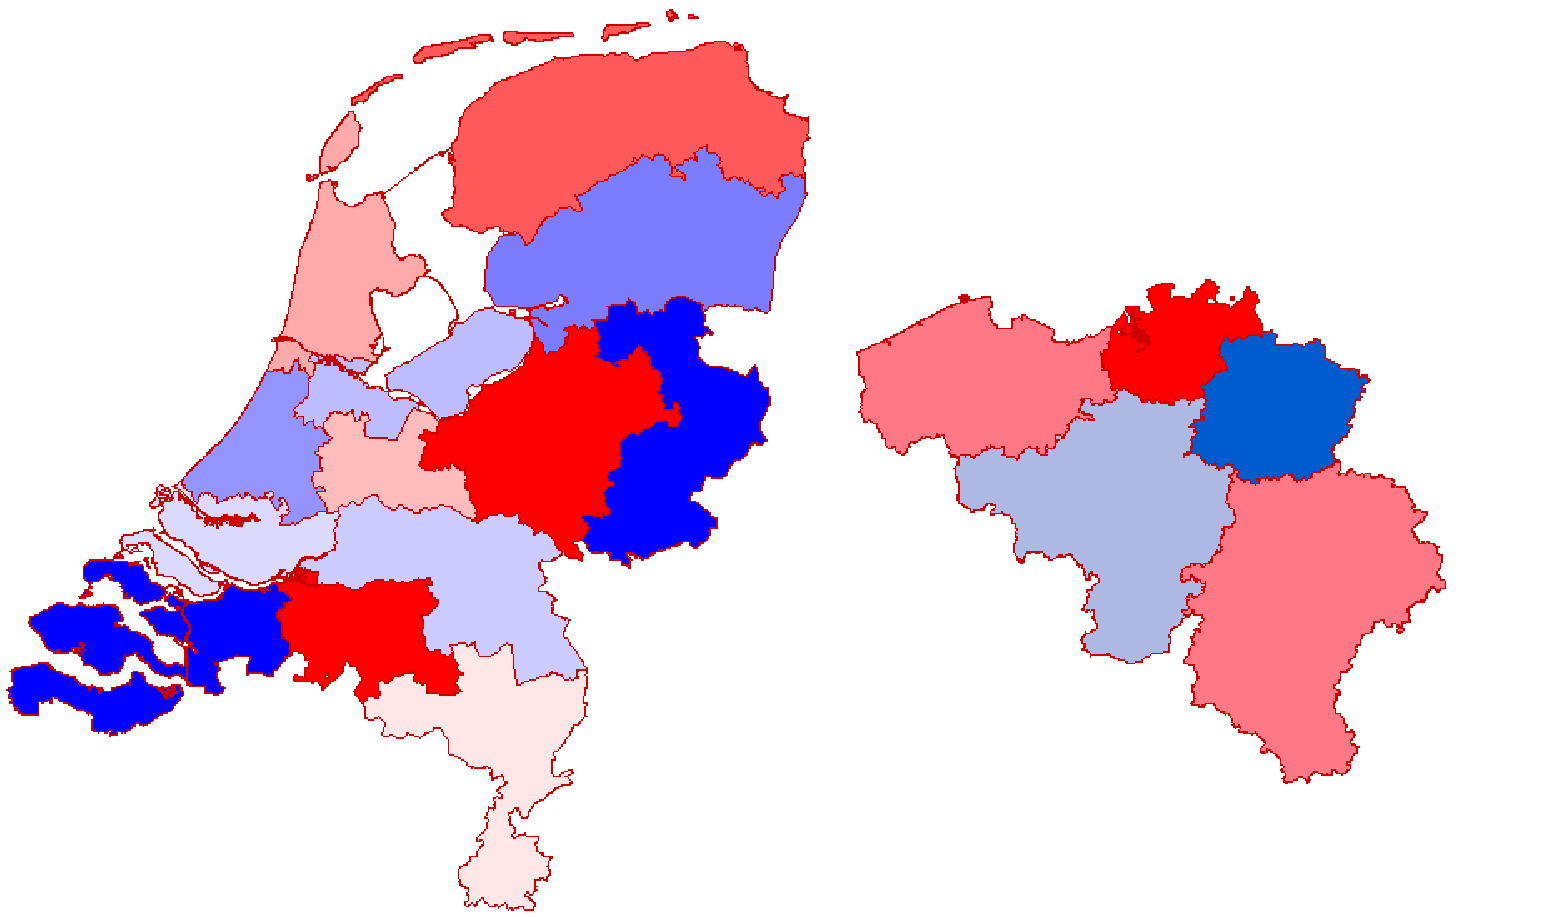
\includegraphics[width=0.8\textwidth]{img/transmission_regions.pdf}
  \caption{The regions serviced by the transport and distribution companies within the TransMission group . The depot located in Luxembourg services the South-East of Belgium and the whole of Luxembourg.}
  \label{fig:regions}
\end{figure}

TransMission uses different types of trucks and trailers and many of their depots can be used as cross-docks.
Line hauls are used to move cargo between depots during nights. Depots pick up and deliver the cargo in their service regions during days. There is a long-term centrally planned set of line hauls. There is also a set of line hauls that is planned daily  by the depots themselves.
TransMission would like to to produce its transport plans every day using all information available to the depots.
 % optimize its planning centrally on per day basis.
To achieve this, producing the transport plan needs to become automated.



\subsection{Scope}

TransMission's problem is an extremely rich one.
The first step to solve a problem is to model it properly.
% The first step to solving a problem is properly modeling it.
It is a pick up and delivery problem without fixed assignments of trailers to lorries where goods can be transfered between vehicles before they reach their destination.
% Furthermore, goods can be transfered from one vehicle to another before it reaches its destination.
\\


In \cite{masson2013adaptive} results are reported on the pickup and delivery problem with transshipments.
In this paper the available fleet is homogeneous and does not contain trailers.
The VRPTT considered in \cite{drexl2007some} only deals with collecting one homogeneous good, instead of picking up and delivering various goods to various locations.
Both works do not cover all features of TransMission's problem.
Of these two models, the VRPTT has been estimated to be the best basis for a model for TransMission's problem.
Its potential to model a wide class of problems has already been demonstrated in \cite{drexl2013applications}.\\

% The main reason TransMissions problem is hardThe loose coupling of trailers and lorries combined with load transfers and a heterogeneous fleet make TransMissions problem difficult to model.

% The VRPTT proposed by Drexl in \cite{drexl2007some} as the best candidate to serve as a basis for the solution to TransMission's problem. Its potential to model a wide class of problems has already been demonstrated in \cite{drexl2013applications}.

Powerful algorithms for solving the VRPTT do not exist yet \cite{drexl2014bandc}.
Stochastic optimization methods and/or heuristics may offer solutions in cases where solving problems exactly is too slow.
Developing such an algorithm is therefore the most logical first step towards solving TransMission's problem. This task is the scope of this thesis. The optimization method will be a simplified version of the ALNS, namely a variable neighborhood search (VNS). The ALNS  has shown promising results on large instances in \cite{masson2013adaptive}.\\

 How the results of this thesis will be used to automate the production of transport plans for TransMission is outside the scope of this thesis.




\subsection{Methodology}
%work transmission
A week was spent within TransMission to work in different departments in order to gain  domain knowledge.
The problem was defined and the scope was determined in collaboration with TransMission.\\

%programming
The python programming language \cite{vanpython} was used to make the algorithm since it allows for rapid prototyping and easy visualizations.
The Numpy package \cite{numpy} was used for fast array computations.
 The  Numba library \cite{analytics2014numba} was used to speed up performance-critical parts of the algorithm.
 Instances provided in \cite{drexl2007some,drexl2011branch} were used to analyze the performance of the algorithm.

\subsection{Outline}
This section provides the problem under consideration with context.
Section \ref{chap:The Problem} explains the problem and formulates the model.
 % the problem and describe its complexities.
%We look at the theory on which our optimization method is based in chapter \ref{chap:Theory}.
In Section \ref{chap:Optimization} all parts of the optimization method are explained.
 % that was used to generate results.
The test methods and the results that were produced by the optimization method are described and interpreted in Section \ref{chap:Tests and Results}.
In Section \ref{chap:Discussion and Future Work} conclusions are drawn and  Section \ref{chap:future-work} outlines promising  directions of this area of research.
 % about future directions and/or opport of this line of research.
% \todo{update this subsection in the end}


\newpage
\section{The Problem}
\label{chap:The Problem}

 \subsection{Problem Description}
 % where does the problem arise from? problem transmission has
 %keep it short, dont go into details that tjalma can disagree with in particular about the operational part.

%%%%%%%%% IMPORTANT HERE YOU ARE!!! ############
% why even talk so much about transmissions problem. Is it relevant for what you try to show in this paper? no! Do you even clearly know the details of the problem so precisely that tjalma and gerard don't disagree with it? DO THEY??!!! remove all this talk about TransMisson. Totally Unnecessary

% overview
The VRPTT can be described as follows:
There is a set of customers with a known, deterministic supply of a single good.
There is a set of transshipment locations that may be used for parking and load transfers.
All locations have opening and closing times.
To collect the customers' supply, a fleet of heterogeneous, limited-capacity vehicles stationed at the vehicle depot is available.
Some customers can not be visited with trailers because of accessibility constraints.
While goods are collected, costs should be minimized.
A lorry ends its path if it unloads at the depot or after it decouples a trailer at the depot. \\

% fleet
The fleet of vehicles consists of lorries and trailers.
Trailers can only move if pulled by a lorry.
Not all trailers and lorries are compatible with each other.
All vehicles may have different capacities, fixed costs and variable costs.
Lorries may differ in the amount of time they need to collect a certain amount of customer supply.  There is no fixed assignment between trailers and lorries.
Trailers can be shared by multiple lorries.
Any trailer can be pulled by any compatible lorry. \\

% locs
Transshipment locations can be used by lorries to transfer load to a trailer.
There are no costs associated with coupling and uncoupling a trailer except for the cost incurred by the time it takes to finish the operation.
A vehicle will start and end its route at the depot location.

% customer
Customers that can not be visited with trailers are called lorry customers. Customers that can be visited with trailers are called trailer customers. Split collections are not allowed, hence each customer's supply is collected by one lorry.
There is no customer with a supply greater than the capacity of the lorry with the least capacity.
Trailer customer locations can also be used as transshipment locations. \\


% NP-hardness

The VRP is a special case of the VRPTT, namely an instance without transshipment locations and without trailers. Since the VRP is NP-hard \cite{laporte2009fifty}, the VRPTT is also NP-hard.



\subsection{Problem Model}

% NOTE change the language of this first part. What could a solution to the question look like. What information does it need to contain?

A solution to an instance of the VRPTT should answer the following questions:
%\begin{itemize}
%\item Which lorry collects the supply of which customers and in what order?
%\item In what order does the lorry collect the supply of customers or couple and decouple trailers?
%\item From where to where is which trailer pulled by which lorry?
%\item Which lorry is coupled to which trailer during which part of its path?
%\item When and how much load to lorries transfer to trailer?
%\item At what time does everything take place?
%\end{itemize}

\begin{itemize}
\item How should the customers be divided over the lorries and in which order should the lorries visit them to collect the customers' supply?
\item How should the lorries use the trailers?
\item How should the load be divided between the vehicles?
\item When do all the events in the plan take place?
\end{itemize}


% A usable model will be able to represent the  answers to these questions.

\subsubsection{Simple Example}

\label{sec:simple-example}

Let us explore a simple example of the VRPTT.
In Figure~\ref{fig:trivial} we can see an illustration of a VRPTT.
For the moment we ignore some aspects of the VRPTT for the sake of clarity.
The VRPTT does not allow a vehicle to leave the depot after it visits the depot.

% Furthermore, instead of asserting the factors that need to be adressed, we could show hwo they arise from the example.
% maybe even make this subsection the first subsection in this chapter. The adept methodology says to first analogy, diagram, experience. Only then give plain english and then technical.
%technical is problem formulation subsecion.
%Plain english resembles problem description section.

\begin{figure}[!ht]
  \centering
    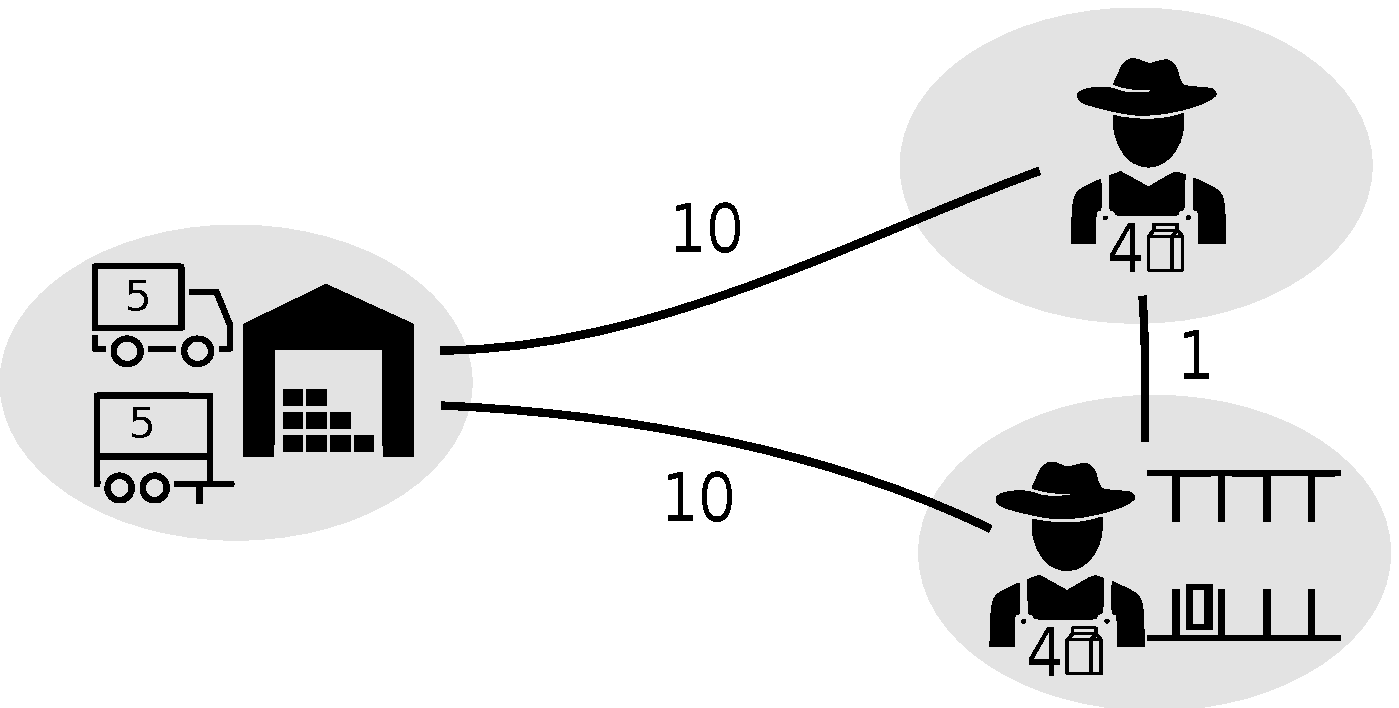
\includegraphics[width=0.8\textwidth]{img/trivial_example_withcapacity_v2.pdf}
  \caption{Illustration of an VRPTT with a trailer customer, a lorry customer and a fleet consisting of a trailer and a lorry.}
  \label{fig:trivial}
\end{figure}

% disclaimer simplification

%%%%%%%%%%%%%%%%%%%%%%
 % explain situation.
 %%%%%%%%%%%%%%%%%%%%%


% locations and fleet
The example problem contains three locations.
One of the locations is the depot.
At the depot there is a fleet consisting of a lorry and a trailer.
The other two locations are customers.
Both customers have a supply of four that needs to be collected by the vehicles and needs to be unloaded at the depot.
Both vehicles in the fleet have a capacity of five.
% distance
The customers are at a distance of one of each other and at a distance of ten to the depot of the transporter.\\

% capacity

% lorry vs trailer customer
The customer on the bottom has a parking lot, hence it has enough space to be visited with a trailer.
This customer is therefore called a trailer customer.
A location that can be visited with a trailer can be used to park a trailer and/or to transfer load from a lorry to a trailer.
Such a location is called a transshipment location.
The other customer does not have a parking lot and can therefore not be visited with a trailer, which makes it a lorry customer.\\

% model choices

% The VRPTT does not allow a vehicle to leave the depot after it visits the depot.
% The lorry can therefore not collect the supply of one customer, then unload and then service the other customer.
 % hence both customers can not  the same lorry can not be used to service both customers.
% A trailer will be immediately unloaded after a lorry decouples it at the depot and can therefore not leave after being decoupled at the depot.


% components of solution
% The transporter would like to know how he should use his fleet to collect the supply of the customers.

\subsubsection{Events}


Let us attempt to construct a plan that answers at least the first two questions that a solution to the VRPTT needs to answer.
Since vehicles are not allowed to leave the depot after visiting it, the lorry can not unload at the depot between visiting the customers.
The lorry and the trailer can not separately take care of a customer, since the trailer can not move on its own.
Since the lorry alone does not have enough capacity to collect the supply of both customers, it needs to use the capacity of the trailer.
%  transfer some of its load that it collects from to the  the capacity of the trailer in some way.
% visit the customers whilst coupled to the trailer.
% couple the trailer and p.
\\

%The trailer cannot move on its own, therefore we do not need to state its movement explicitly. It is defined by the actions of the lorry.

The lorry can not visit the lorry customer whilst coupled to the trailer.
% and the trailer can not visit the lorry customer together.
Let us say that they go to the trailer customer first. So far the plan is as follows:
\begin{enumerate}
  \item The lorry starts it path at the depot.
  \item The lorry couples the trailer.
  \item The lorry and trailer drive to the trailer customer.
\end{enumerate}
Now there are two good courses of action.
Either the lorry collects the supply of the trailer customer first or it decouples and parks the trailer first such that it can collect the supply of the lorry customer.
Let us say that it collects the supply of the trailer customers first, then the plan continues as follows:
\begin{enumerate}[resume]
  \item The lorry collects the supply of the trailer customer.
  \item The lorry transfers at least three units of the supply to the trailer such that it has at least four capacity available for the supply of the lorry customer.
  \item The lorry parks and decouples the trailer.
  \item The lorry drives to the lorry customer.
  \item The lorry collects the supply of the lorry customer.
  \item The lorry drives back to the trailer customer.
  \item The lorry couples the trailer.
  \item The lorry drives back to the depot.
  \item The lorry decouples the trailer and unloads.
  \item The lorry ends its path and unloads.

\end{enumerate}

% notice how the activities that the lorry is involved in completely defines what happens to the trailer.

This is quite a verbose description of a transport plan.
Notice that every step is either about the lorry travelling between locations or about the lorry performing an activity at a location.
% the (change of) location of the lorry (and trailer) or about an activity the lorry undertakes at a location.
This list of steps can be compressed into a list where every step consist of an activity and a location, see Table~\ref{tab:events}.
From now on this combination is called an event. The sequence of events that a lorry is involved in is its path.

\begin{table}[!h]
  \centering
  \begin{tabular}{@{}llll@{}} \toprule
  %  \multicolumn{2}{c}{Event} \\ \cmidrule(r){1-2}
    Event \# & Location & Activity & Event ID  \\ \midrule
    1 & depot & start path & A \\
    2 & depot & couple the trailer & C \\
    3 & trailer customer & collect supply & F \\
    %4 & trailer customer & transfer load & lorry and trailer \\
    4 & trailer customer & decouple the trailer & G \\
    5 & lorry customer & collect supply & E  \\
    6 & trailer customer & couple the trailer & H  \\
    7 & depot & decouple trailer & D  \\
    8 & depot & end path  &  B \\     \bottomrule
  \end{tabular}
  \caption{The events in the plan.}
  \label{tab:events}
\end{table}

Notice that the load transfer from the lorry to the vehicle is not treated as a separate event.
This is because we allow the load to be transfered from the lorry to the trailer at any event as long as they are coupled.
In this case the transfer happens in either event three or four and the amount that is transfered lies between three and four such that the lorry has enough capacity to collect the supply of the lorry customer.\\
% Later in more detail how the transfer of load is represented from the lorry to the trailer.
 % on that we can determine how to divide load between lorry and trailer without using such an event in our model.

Notice also that by choosing to park a trailer, two events are created. A trailer needs to start and end its path at the depot, hence if it is decoupled at some transshipment location it needs to be coupled again there as well. \\






\begin{figure}[!h]
  \centering
    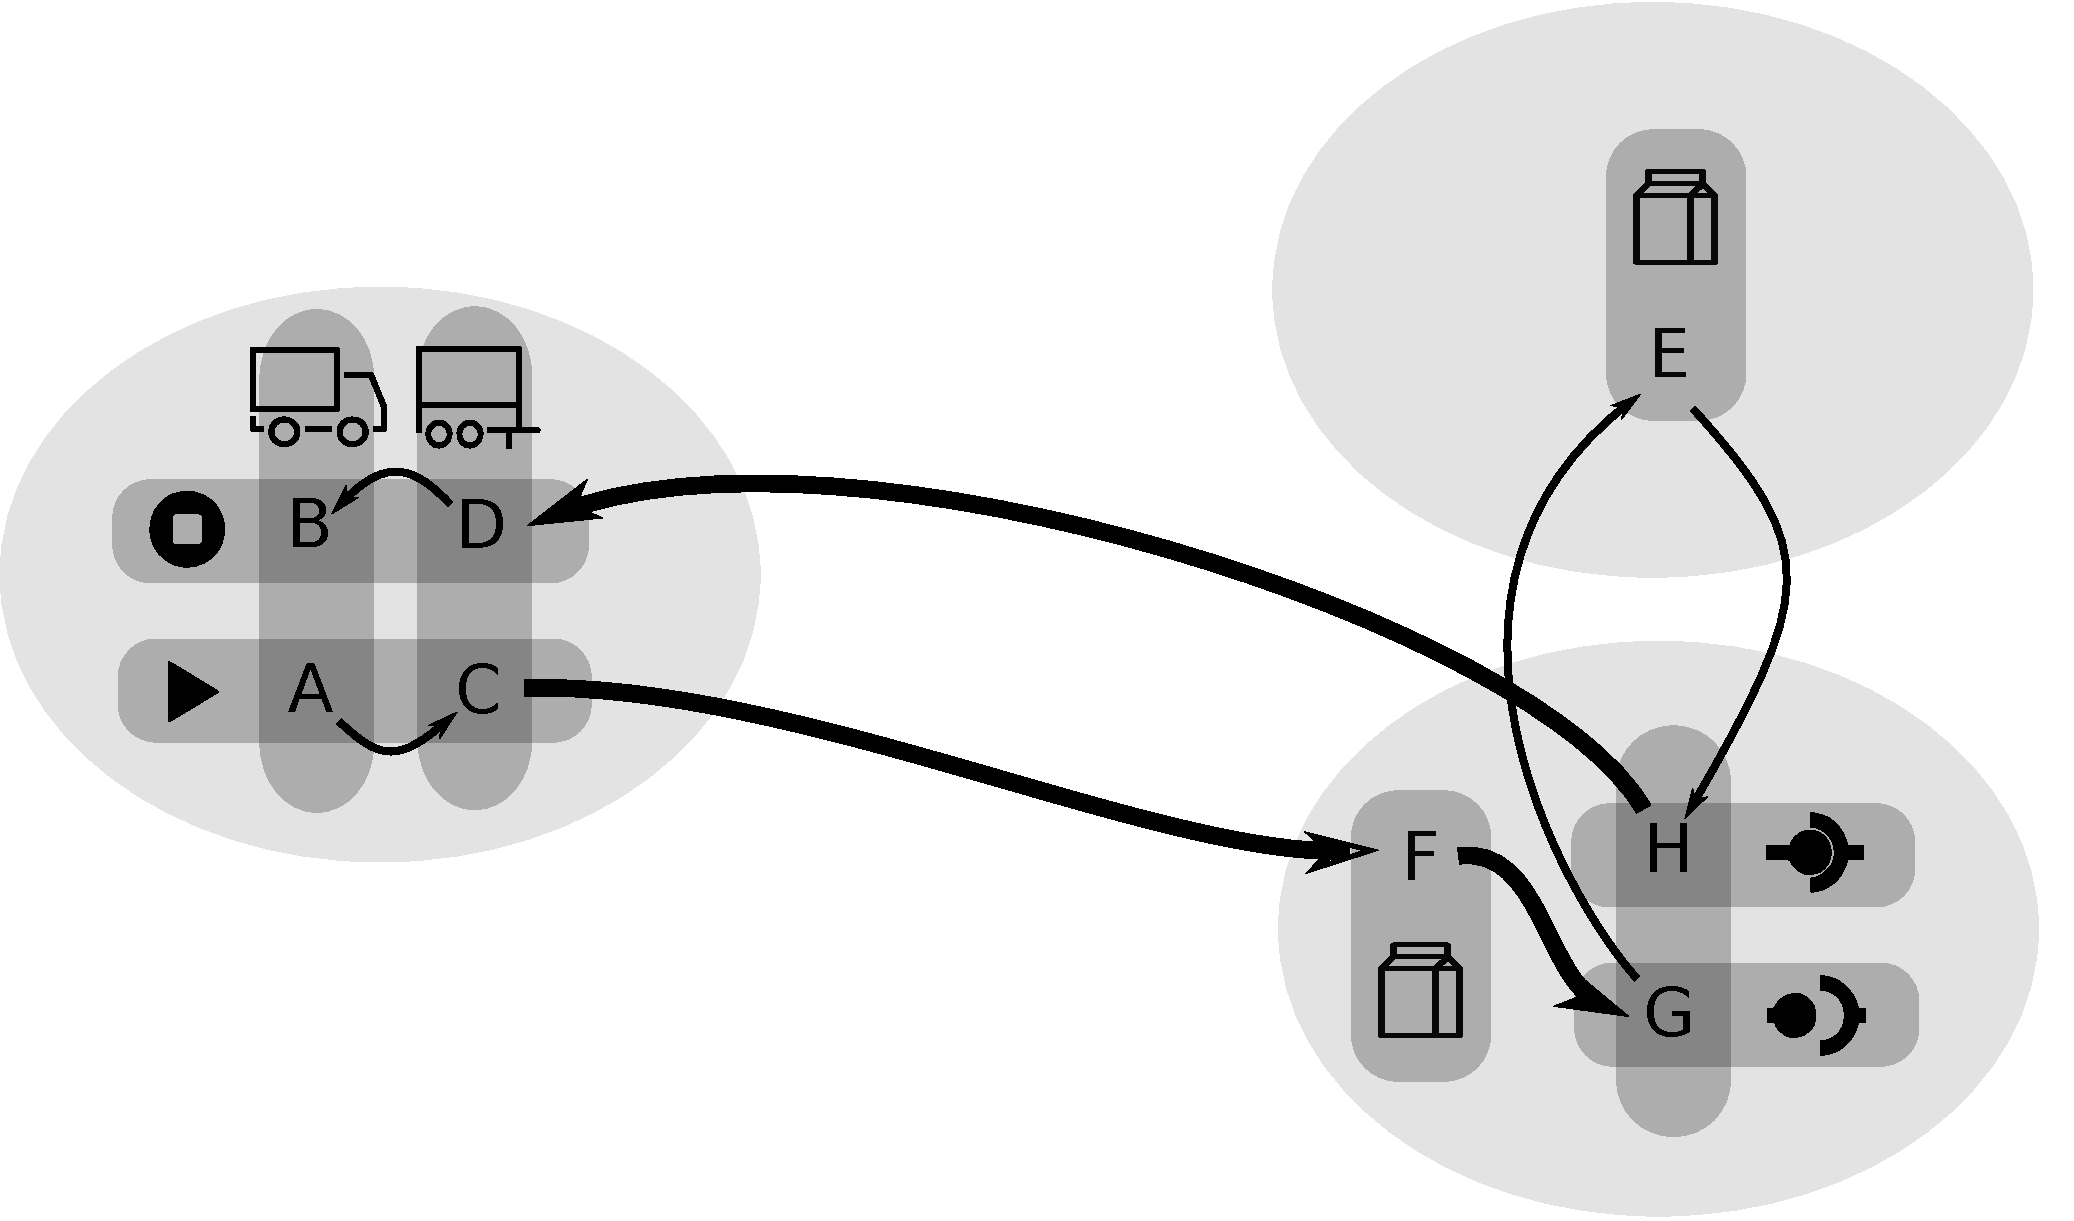
\includegraphics[width=0.8\textwidth]{img/trivial_vertices_v2.pdf}
  \caption{An illustration of the lorry's path. Every event is indicated with the event ID supplied in Table~\ref{tab:events}. The activity of the event is illustrated with a symbol. The position indicates the location of the event. The fat lines indicate where the lorry is coupled to the trailer. The thin lines indicate where the lorry is not coupled to the trailer.}
  \label{fig:vertices}
\end{figure}



If we look at Figure~\ref{fig:vertices} we can see all the events in our plan and the path of the lorry.
From the path of the lorry we can infer the path of the trailer, namely it starts at $C$, then we follow the fat line to $ F $ and $ G$. Transshipment events come in pairs, a couple event and a decouple event. A trailer decoupled at $G$ can be coupled again at $H$.
 % This is a movement through time, not space.
 From $H$ we follow the fat line back to $D$. \\

Notice that each event in the plan is unique, in that it occurs only once in the path of the lorry.
% by constructing the plan in terms of events every element of the plan only occurs in the path of the lorry once.
Furthermore, notice how we can answer the first two questions that a solution to the VRPTT needs to answer by looking at the path of the lorry.


\subsubsection{Load Division}

% The capacity of the vehicles is limited.
% Given the path of the vehicles, how should we use their capacity such that the supply of the customers can be collected and unloaded at the depot whilst not overloading the vehicles?\\

The third question that needs to be answered is about how, given the events of a plan, the customer supply ends up at the depot.
 % by flowing through the vehicles.
% flows from the customers through the vehicles, to the depot.
The vehicles have a limited capacity, so they need to coordinate how load is divided between them.
This is done by determining at which event of the plan a load transfer from a lorry to a trailer needs to take place and the amount that needs to be transfered.
% the amount of load that needs to be transfered from a lorry to a trailer, and the event at which this needs to happen.
\\




%  load flows from customers to the depot.
% This is the third question a solution to the VRPTT needs to answer.
% Furthermore, is it even possible to collect all the supply without overloading the vehicles given the paths of the vehicles?

% To determine this we need to track the flow of the load from the customers to the depot.


\begin{figure}[!h]
  \centering
    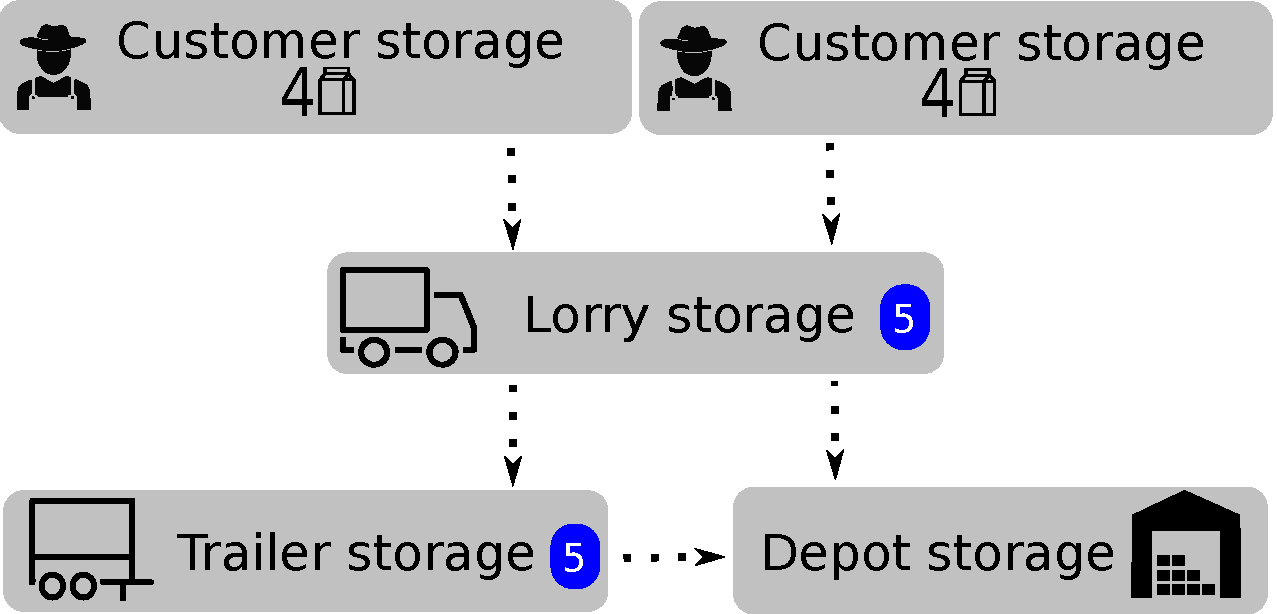
\includegraphics[width=0.8\textwidth]{img/trivial_flow_simplified_v2.pdf}
  \caption{An illustration representing how load can flow from the customers to the depot. The amount of supply of the customers is indicated with the milk icon and the capacity of the vehicles is indicated in blue. }
  \label{fig:flow_simplified}
\end{figure}

The customers' supply flow from customers to the depot as presented in Figure~\ref{fig:flow_simplified}.
The only sources of supply are the customers, both with a supply of four.
The only sink for the load is the depot.
The supply can reach the depot by flowing from a customer to the lorry and then to the depot.
Alternatively, supply can flow from a customer to the lorry, then to the trailer, then to the depot.
Before the vehicles can be finished with collecting all eight units of customer supply, at least three units of supply must have flown to the trailer, since the lorry can only hold five units of supply at any one time.
No more than five units of supply can have flown to the trailer in total, since it can only hold five units.
Notice how the lorry can decrease its amount of load before unloading at the depot, but that the trailer can not.  \\

% Before all of the supply of the  supply of the second customer can be collected at least some of the load has to flow to the trailer.  since the sum of the customer supplies (eight) is greater than amount of load that the lorry can hold at once (five).

% The question is: when and how much of the load is transfered to the trailer such that the vehicles ares not overloaded?
% Figure~\ref{fig:flow_simplified} does not offer enough detail to answer this question.
% See Figure~\ref{fig:flow} for greater detail.



\begin{figure}[!h]
  \centering
    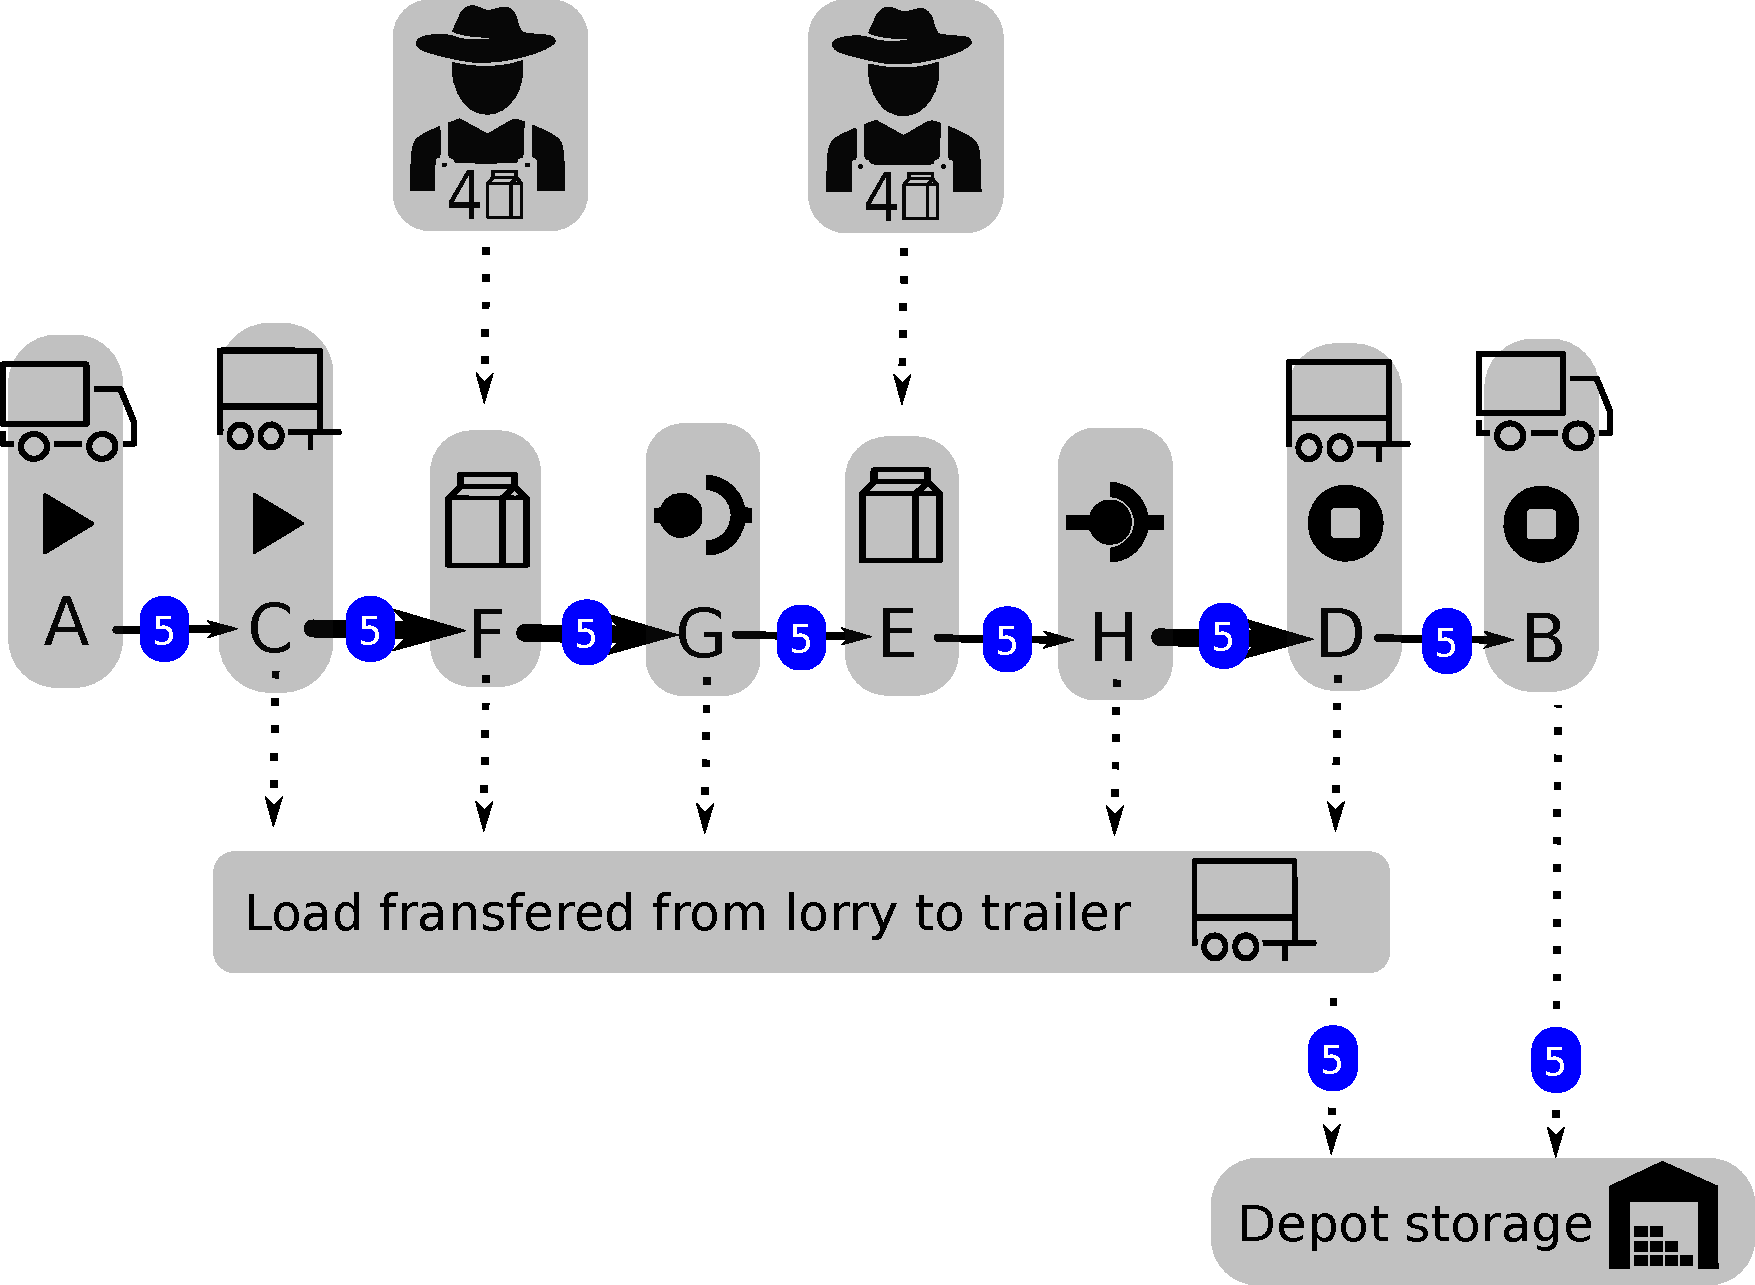
\includegraphics[width=0.8\textwidth]{img/trivial_flow_v2.pdf}
  \caption{The load division problem. Dashed arrows represent the ways that load can flow. If flow restrictions exist, they are indicated in blue.
 Arrows indicate how load can flow from event to event as cargo inside the lorry.
 Fat arrows indicate when the lorry is coupled to the trailer.}
  % The amount of customer supply is indicated with the milk icon.}
  \label{fig:flow}
\end{figure}

To not only determine the amount of supply that needs to be transfered, but also the event at which the transfer needs to take place, we need to consider the flow of supply per event. The ways supply can flow at each event is illustrated in Figure~\ref{fig:flow}.
Every time the lorry is at an event, it can choose to transfer load to the trailer, if they are coupled.
% In Figure~\ref{fig:flow} we see all the events in the path of the lorry.
% At the events where the lorry is coupled to the trailer, load can flow from the lorry to the trailer.
At the supply collection events, $F$ and $E$,  load can flow from a customer to the lorry.
When the lorry ends its path at the depot, event $B$, load can flow from the lorry to the depot.
The only time load can flow out of the trailer is when it decouples at the depot, event $D$.
The maximum amount of load that can flow from a vehicle to the depot is equal to its capacity, which is five for both vehicles.
We can ensure that the trailer is never overloaded during its path if we constrain the amount of flow from the trailer to the depot to the trailer's capacity, since that is the only time that load can flow out of the trailer.
Load can flow into and out of the lorry at multiple events, therefore we have to restrict the flow between events to the lorry's capacity such that during its path it never carries more load than its capacity.
\\



%Lets look at Figure~\ref{fig:vertices} and imagine how the supply of the customers can flow from the customers, %through the lorry and possibly through trailer, to the depot. Keep in mind that the fat line indicates where the %railer and lorry are coupled, and that the lorry can transfer load to the trailer at any event where they are %coupled. This situation is summarized in Figure~\ref{fig:flow}.




% TODO To check this in a more systematic way instead of eyeballing, we turn this problem into a weighted digraph using thefollow trick and use a max flow algorithm.


%
% We can eyeball that if the supply of the customer that is visited first, flows from the customer to the lorry and then straigth into the trailer and the supply of the second visited customers is just kept inside the lorry, then all the supply of each customer can be collected without overloading any vehicle.
%
% But instead of eyeballing the solution like this, we can also find a solution by solving the a max flow problem.

This problem of dividing load between vehicles can be abstracted to a maximum flow problem, see  Figure~\ref{fig:flow_abstract}.
The maximum flow problem asks how much load can transfer from a source to a sink.
The vertices of the maximum flow problem consist of the events of the plan, a special vertex $P$ for the trailer to show the flow of load from the lorry to the trailer,
one sink $sink$ and one source $source$.
% A max flow problem has vertices, capacitated edges and one source and one sink.
We already have one sink, which is the depot.
However, we have two sources of supply, which we replace with one source.
The source has an edge to a customer's supply collection event with a capacity equal to the customers amount of supply, such that the maximum amount of supply that can be collected at the customer's is maintained.
We have already determined where and how much load can flow, which is reflected in the rest of edges and the edge capacities. \\
% The edges reflect how supply can flow between the vertices with capacities that reflect how much load can flow over the eg.
% To represent load flowing to the trailer we have added the vertex


% In our situation we have two sources.
% We can change this by adding a supersource $S$ connected to the customers $S'$ and $S''$  and by restricting the flow from the supersource to the customers to the amount of their supply.



\begin{figure}[!h]
  \centering
    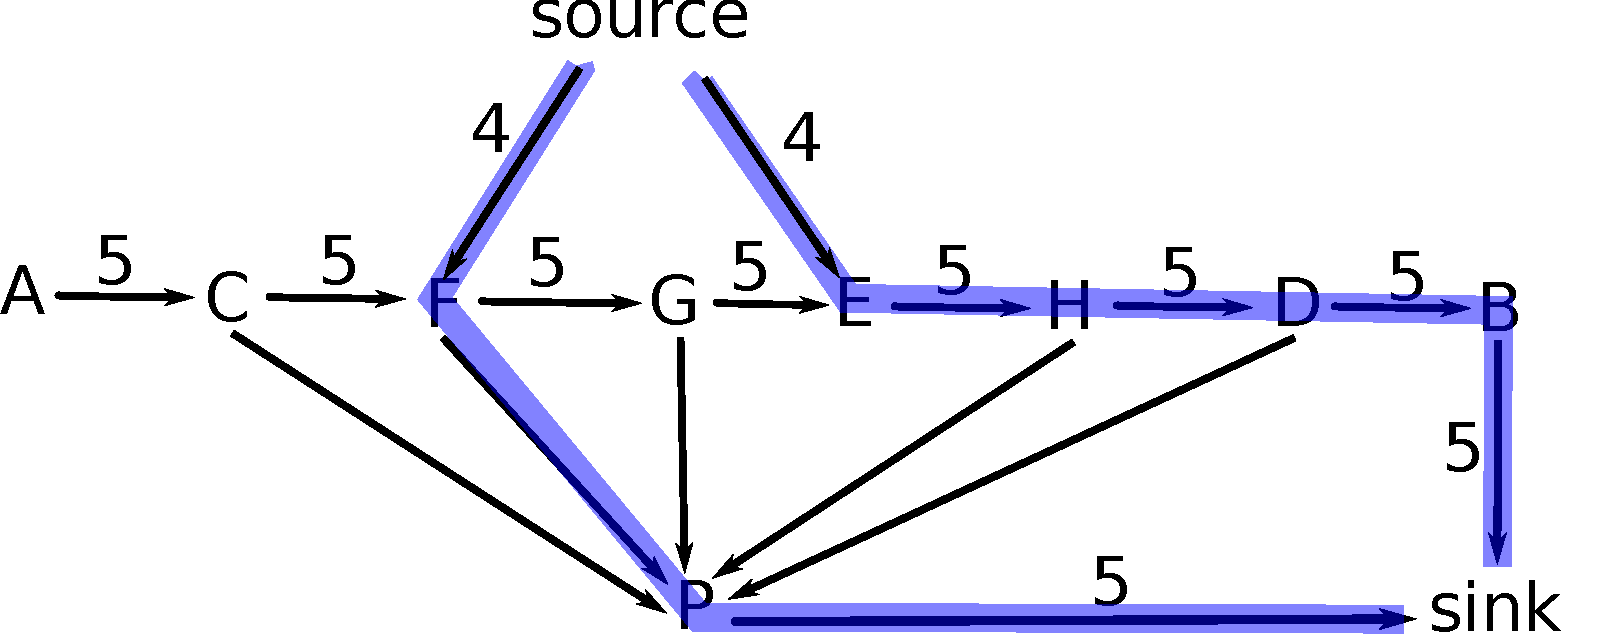
\includegraphics[width=0.8\textwidth]{img/trivial_flow_abstract_BlueFlow_v2.pdf}
  \caption{A directed graph representing the load division problem. If an edge has a limited capacity, the capacity is shown.}
  \label{fig:flow_abstract}
\end{figure}

% In Figure~\ref{fig:flow_abstract} we illustrate the situation as a graph with a few changes.
%
% Load that is transfered to the trailer, flows to vertex $P$. This vertex is sort of a pool which gathers all the load that gets transfered from the lorry to the trailer.


% This would result in the load table of Table \ref{tab:loadtable}. The load table describes how much load a lorry has when leaving an event. \\

%
% \begin{table}[!h]
%   \centering
%   \begin{tabular}{@{}lllll@{}} \toprule
%   %  \multicolumn{2}{c}{Event} \\ \cmidrule(r){1-2}
%     Event \# & Location & Activity & Event ID & Load \\ \midrule
%     1 & depot & start path & A & 0 \\
%     2 & depot & couple the trailer & C & 0 \\
%     3 & trailer customer & collect supply & F & 0 \\
%     %4 & trailer customer & transfer load & lorry and trailer \\
%     4 & trailer customer & decouple the trailer & G & 0 \\
%     5 & lorry customer & collect supply & E & 4 \\
%     6 & trailer customer & couple the trailer & H & 4 \\
%     7 & depot & decouple trailer & D & 4 \\
%     8 & depot & end path  &  B & 4\\     \bottomrule
%   \end{tabular}
%   \caption{The load table corresponding to the flow in Figure \ref{fig:flow_abstract}.}
%   \label{tab:loadtable}
% \end{table}
%\begin{figure}[!h]
%  \centering
%    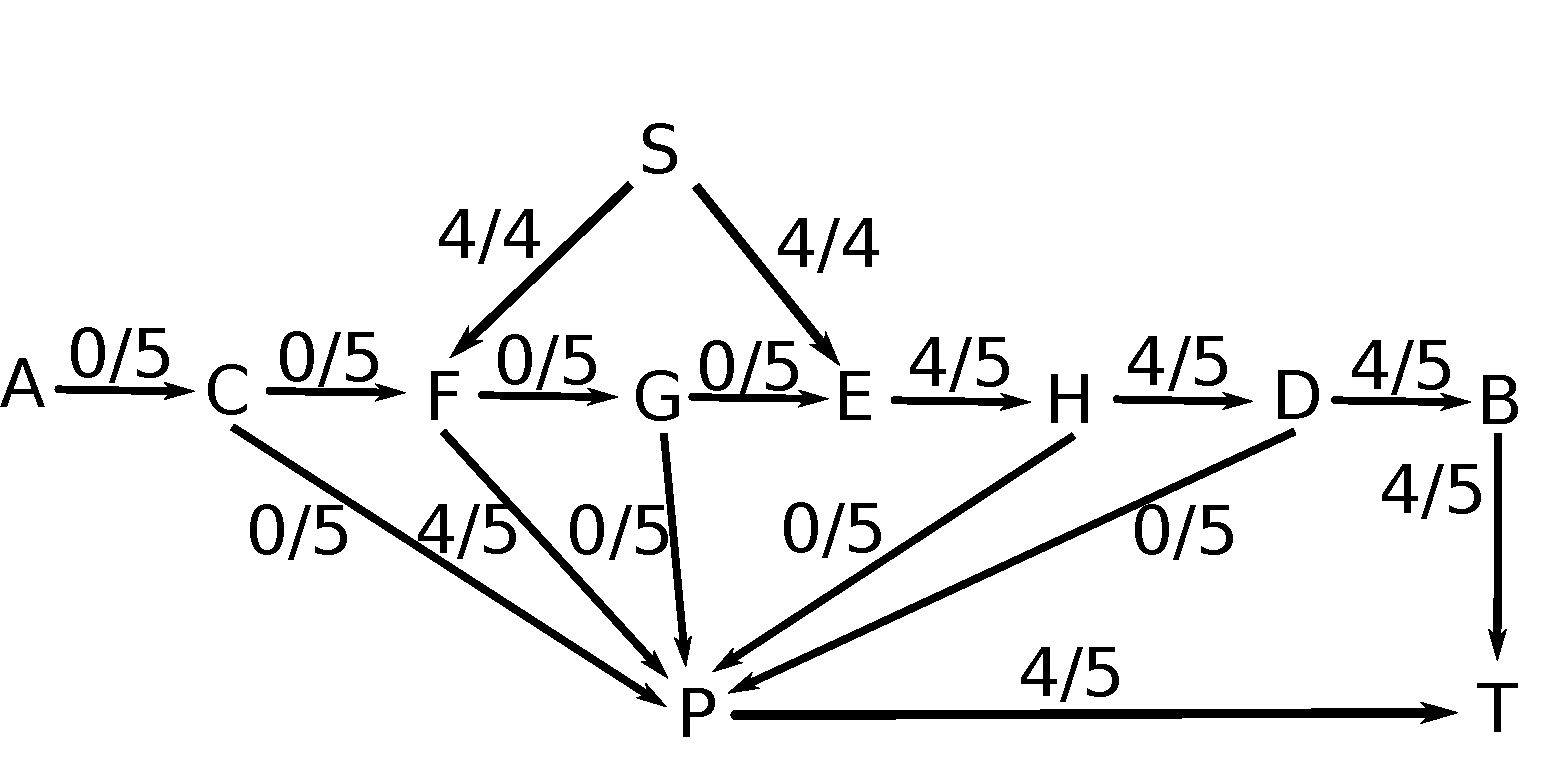
\includegraphics[width=0.8\textwidth]{img/trivial_flow_solution.pdf}
%  \caption{A directed graph with the capacity on the edges and a flow that is a solution to the max flow problem from source $S$ to sink $T$.}
%  \label{fig:flow_solution}
%\end{figure}


A possible solution to this max flow problem is a flow of size four on path $\{S,F,P,T\}$ and a flow of size four on path $\{S,E,H,D,B,T\}$. This is the solution illustrated in Figure~\ref{fig:flow_abstract}.
The third question a solution to the VRPTT needs to answer can thus be solved by solving a maximum flow problem.
%interpret results
% In the suggested solution only at event $F$ which corresponds to collecting load at the trailer customer, a load of size four was transfered from the lorry to the trailer.
% possible
\\

If the maximum flow is smaller than the sum of the customers' supply, we know that given the current event plan no way of dividing the load between the vehicles exists, that would allow us to collect all the customers' supply.
Not creating a separate event for load transfers has enabled us to infer this.
% Being able to infer this is what not creating a separate event for load transfers has done for us.

% answer fourth question
% By looking at the paths of the lorries it can be seen for each event whether and which trailer the lorry was pulling . Given that we know for each event whether and how much load was collected there by the lorry, we can also answer whether and how much load was transfered to the trailer by looking at the load of the lorry at each event.

%\todo{in this case it is easy enough to eyeball how load needs to be balanced such that the lorries have enough capacity to pickup the supply of the customers. And even that it is possible. But how do we formally check this? }





% separate decouple and couple because if I want to assign a time or I want to say that one thing has to happen before something else, I should have 2 vertices. Otherwise it also has 2 successors.



% you don't need separate description of what the trailer does. Everything is described of the lorry taking actions.



%Which components does a transport plan consist of?  In this example the transport plan needs to describe the movements of the lorry and the trailer.



% driving cost
%The cost per distance unit of the lorry and the trailer is one and $0.1$ respectively.


% time parameters
%Lets say that the maximum speed of the vehicles is 1 distance unit per time unit and that it takes 2 time unit to load 5 milk units
%The objective function that we need to minimize is the sum of the HERE YOU ARE!

% what argument can I give for the structure of vertices without invoking time.
% - I could say that to make a solution I need to describe the movement of the vehicles. I can do this even without capacity.


% all information till here is visible in picture. Perhaps first deal with this case and only then introduce the factor time for which the parameters are given below.
% Lets recap: we can answer the first three questions a plan needs to adress by looking at the path of the lorry and by tracking its load at each events on its path.




\subsubsection{Timing }

% In the previous section we talked about the flow of load, now we will talk about the flow of time.
% The flow of time can best be described using a time table that describes the time at which a lorry arrives at an event.
% An event represent a lorry that changes locations or a lorry performing an activity at a location.

% TODO The time at which a lorry arrives at a location can thus be interpreted as the time at which the lorry is ready to start the event.

% The time table describes the starting time of each event.
% A time table indicates at what time a lorry needs to start on its path and
% the duration of the lorry's path can be .
% Another use of a time table is that we can verify whether the paths of the lorries satisfy the time constraints of the locations.

% The fourth question that needs to be answered is about at what time the events of a plan  take place such that costs are minimized and the locations' time windows are not violated. In this example the amount of time that the fleet uses is used as a proxy for costs.
% \\


The fourth question that needs to be answered is about at what time the events of a plan  take place.
It would be preferable if the lorry would take the least amount of time possible to complete its path and start performing each activity as early as possible. 
% and be at each event at the depot as early as possible. 
However, there should be enough time for the lorry to travel between locations,
to perform the activities of the events
and not violate  the time windows of the locations.\\



% .
% At what time should each event take place, such that there is enough time to perform each event, travel between events, such that the time windows are notS violated and the least amount of time is spent just waiting till a location opens. ??Added preference; we would like to do everything as early as possible?? if start and end time are fixed, we would liike to do everything as early as possible (because of slack and because that is just how I defined that it works. Lorry starts as soon as arrives or as sson as openss. does not wait at vertex. also becasue there is no slack than anymore)



\

% , the customer supply ends up at

\begin{figure}[h]
  \centering
    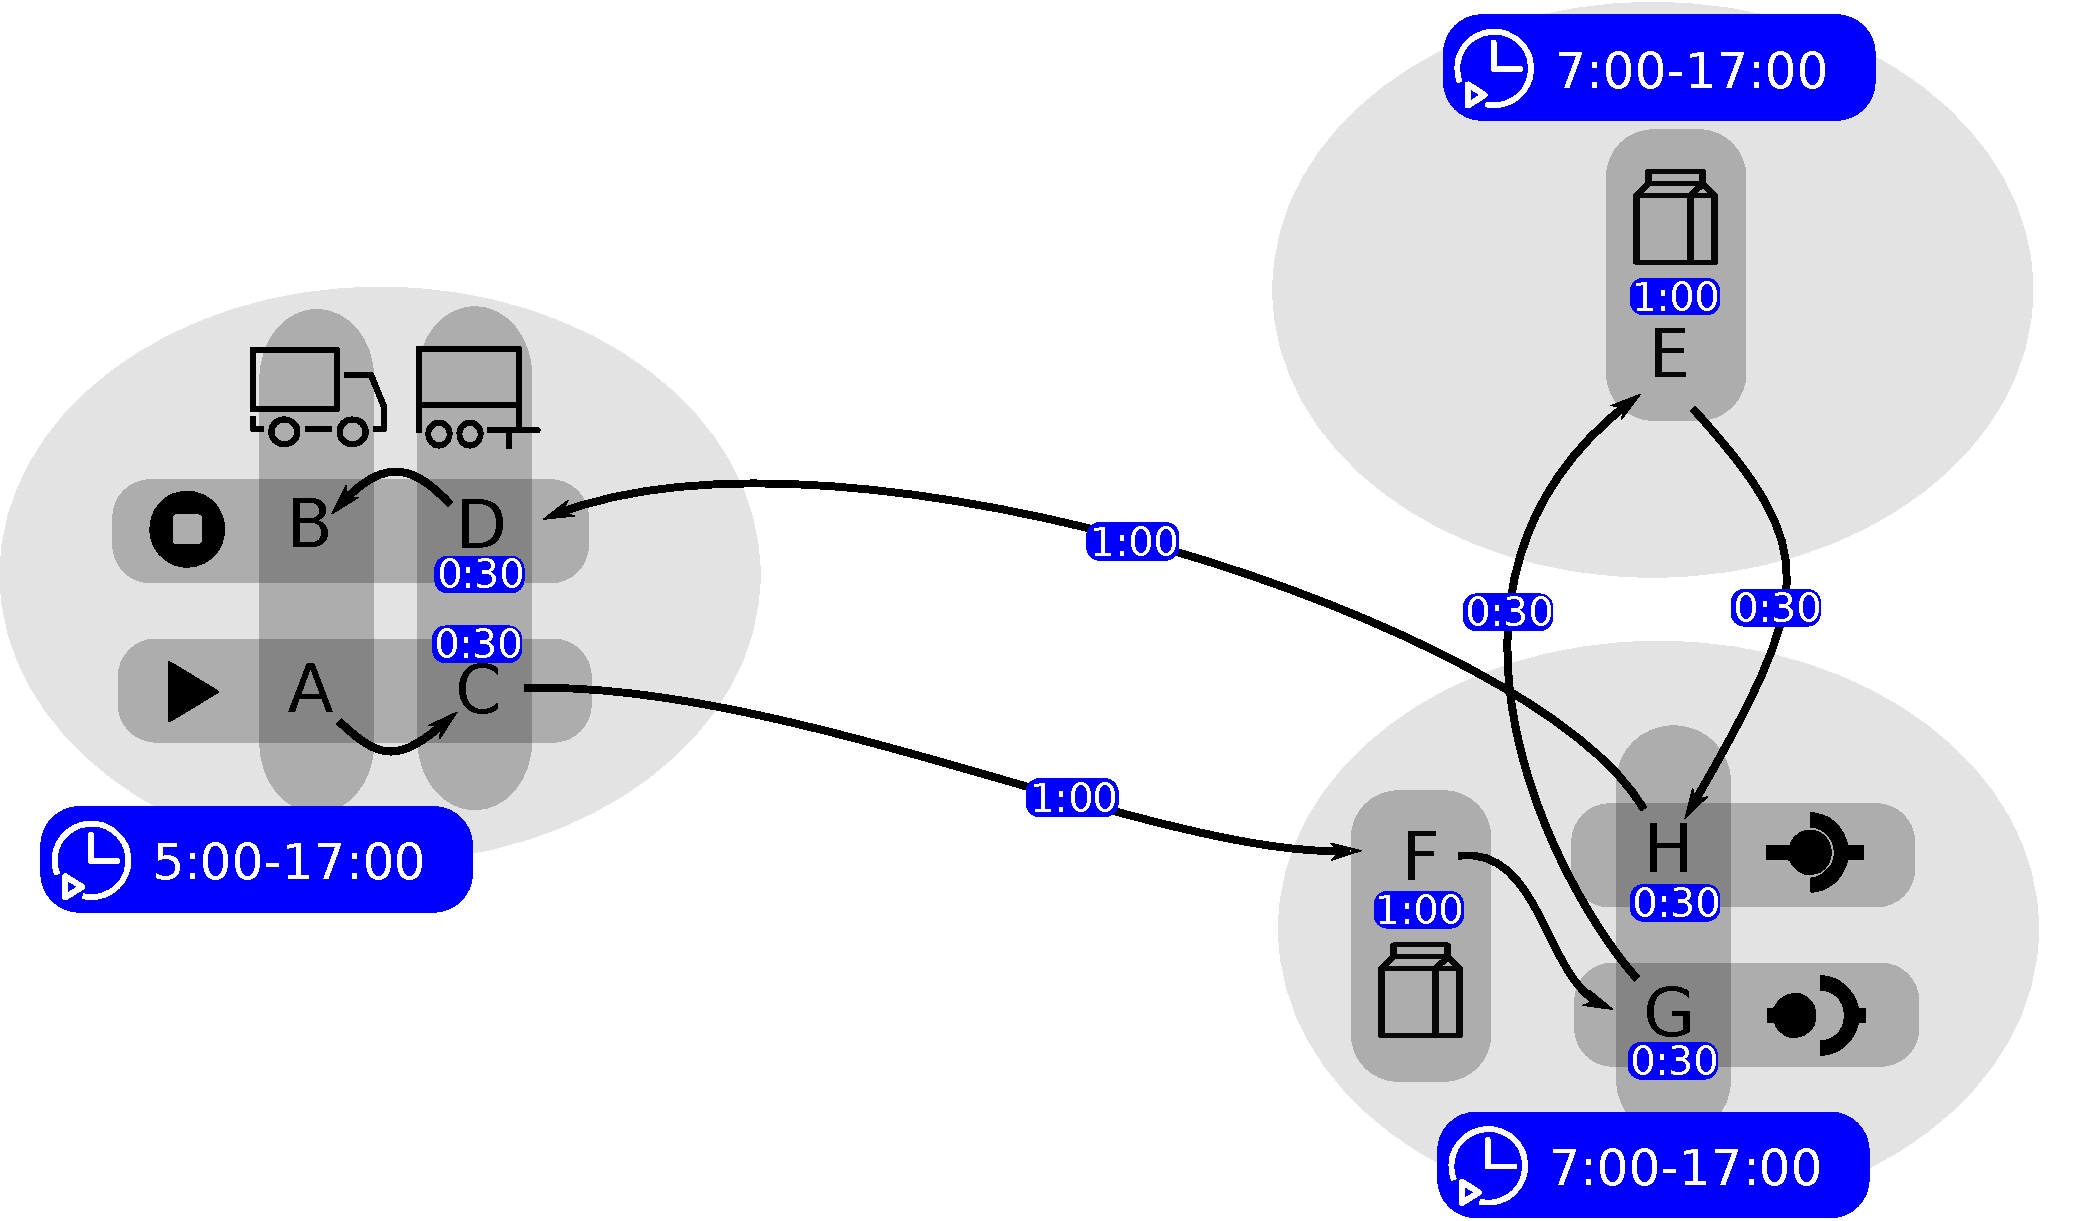
\includegraphics[width=0.99\textwidth]{img/example_with_time_v2.pdf}
  \caption{An illustration of the lorry's path with time information illustrated in blue in hours. Each location has a time window that holds for all events at that location.
 If no time information is provided the travel duration or event duration is zero.
 As Figure ~\ref{fig:graph_time} illustrates, some events don't take up any time and going from event to event on the same location does not take up any time.
  %  If an event has a nonzero duration or if there is nonzero travel time between events , the time is indicated in blue.
   }
  \label{fig:graph_time}
\end{figure}

To illustrate the problem we extend the example of Section \ref{sec:simple-example} with time windows, travel times, event durations and a planning horizon of 0:00 till 22:00 hours.
The rest of the time related information is provided in Figure ~\ref{fig:graph_time}. \\



\begin{figure}[h]
  \centering
    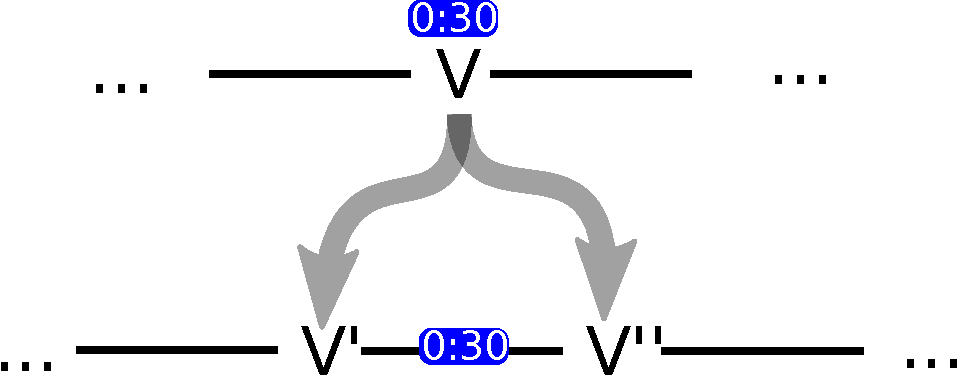
\includegraphics[width=0.6\textwidth]{img/pert.pdf}
  \caption{An illustration of how the duration of an event $V$ is modeled by replacing the event with two other events $V'$ and $V''$ with an edge weight.}
  \label{fig:duplication}
\end{figure}

Similar as the division of load, the problem of timing the events can also be modeled as a graph problem. 
This is done by creating a precedence graph, where edge weights represent the time between events. 
A source and a sink are added to model the beginning and the end of the planning horizon. 
Since some events have a duration themselves each event is first divided into two separate events such that the duration of an event can be represented as the edge weight between the two new events as shown in Figure \ref{fig:duplication}. 
Furthermore, a directed edge is added between the decouple and the couple event at the transshipment location to model that a trailer must be decoupled before it can be coupled again. 
\\





% TODO perhaps I should also make a small example that shows a dynamic time window with 2 lorries. Use this opportunity as well to explain that there can be no cycle.
\begin{figure}[!h]
  \centering
    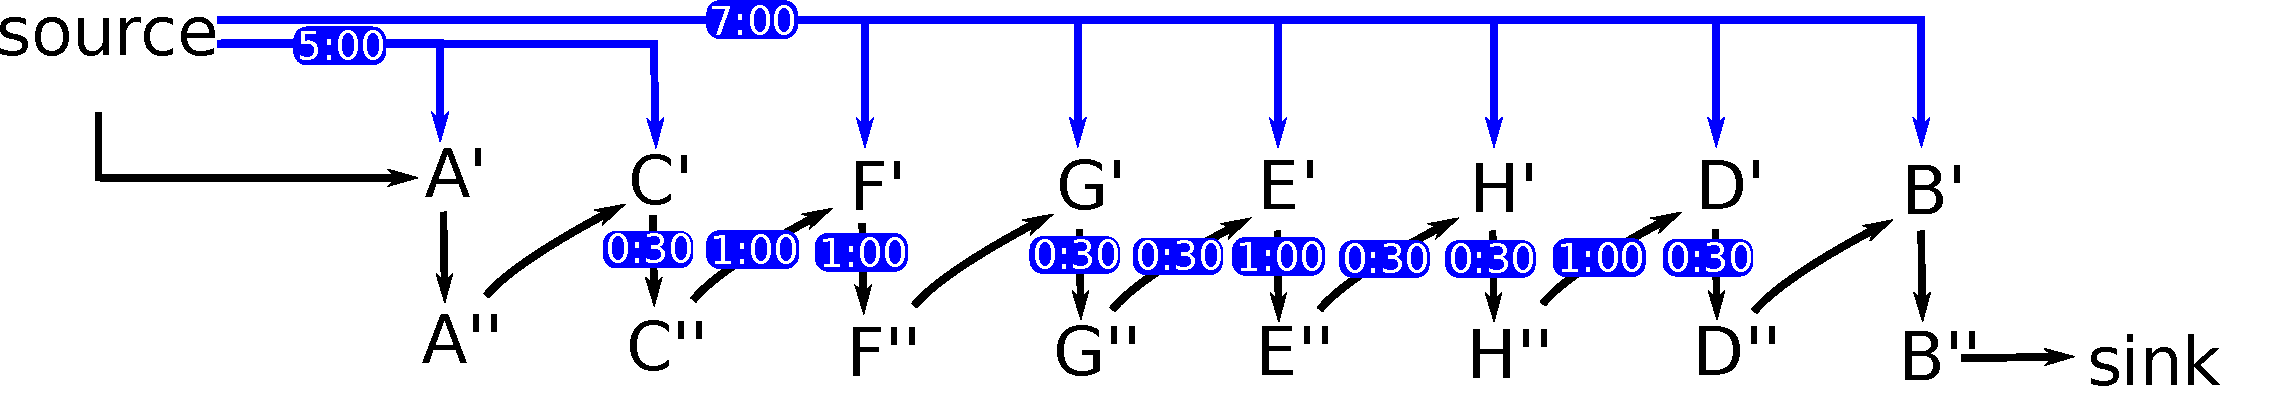
\includegraphics[width=1.0\textwidth]{img/forward_intro_tt.pdf}
  \caption{An illustration of the precedence graph. 
  The edges that model the opening times of the locations at which the events take place are indicated with the blue edges. 
  The black edges indicate the event durations and the travel times between the events. If an edge's weight is not shown it has the value zero. }
  \label{fig:longest_path}
\end{figure}

Let us first try to answer at what time the lorry can finish its path. 
We answer this by performing a longest path search on the precedence graph shown in Figure ~\ref{fig:longest_path}, which also has edges that model the opening times of the locations at which the events take place. 
We see that the longest path $\{ source, F', F'', G', G'', $ $ E', E'',  H', H'', D', D'', B', B'' \} $ from the source to the end of the event that stops the lorry's path, $B''$, is 12:30 hours.
Therefore, the earliest that the lorry can end its path is at 12:30 o'clock.
The path has taken the lorry 7:30 hours. \\

If the lorry start its path as early as possible, 5:00 o'clock, the lorry would arrive at the trailer customer at 6:30 and would have to wait have an hour before it could start collecting the supply. 
We can perform a similar longest path search backwards to see at what time the lorry can start its path whilst finishing its path at 12:30 o'clock.
The longest path search is performed on the antecedence illustrated in Figure \ref{fig:antecedence}. 
The time between the time at which the lorry can end its path at the earliest and the end of the planning horizon is 22:00 - 12:30 = 9:30 hours. \\



\begin{figure}[h]
  \centering
    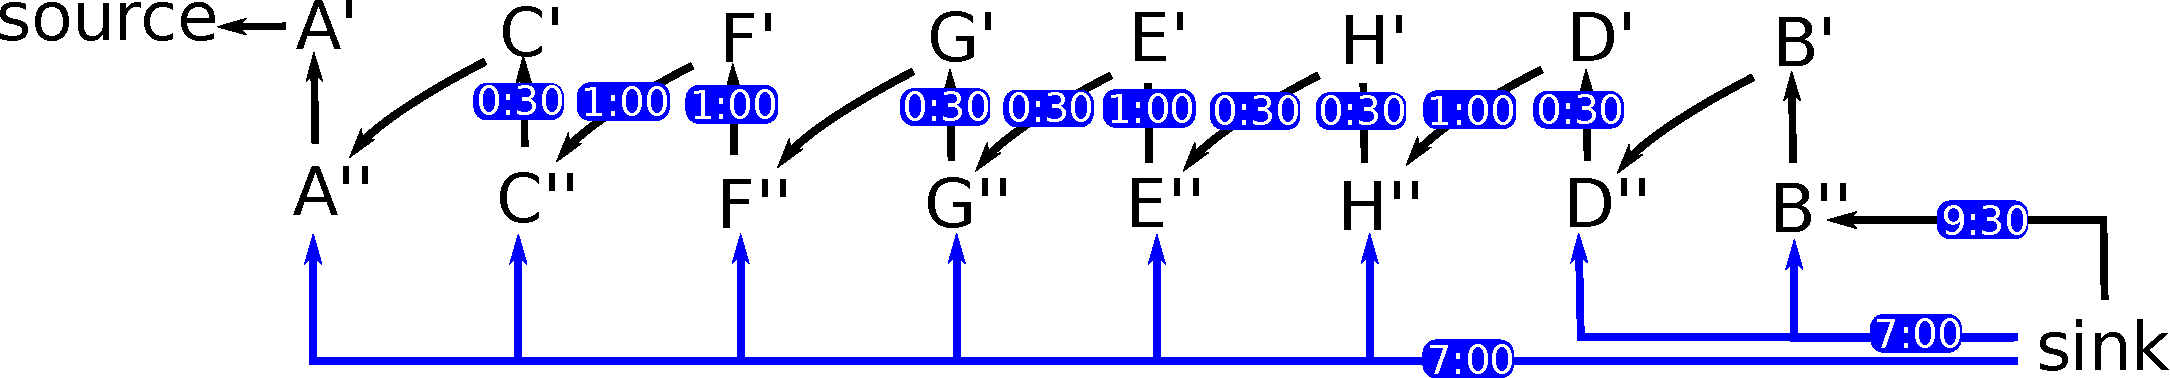
\includegraphics[width=1.0\textwidth]{img/backward_intro_tt.pdf}
  \caption{An illustration of the precedence graph. 
  The edges that model the opening times of the locations at which the events take place are indicated with the blue edges. 
  The black edges indicate the event durations and the travel times between the events. If an edge's weight is not shown it has the value zero. }
  \label{fig:antecedence}
\end{figure}

The longest path in the antecedence graph from the sink to the start of the lorry's path $A'$ is 16:30 hours, hence the lorry can start its path at 5:30 and still end its path 12:30 o'clock. 

We now perform the longest path search on the precedence graph illustrate in Figure \ref{fig:longest_path} again, only this time the edge weight of the edge between the source and $A'$ is 5:30. 
This longest search provides the timing of the events that minimizes the lorry's path duration, schedules activities as early as possible whilst taking into account the travel times, the activity durations and the location's time windows. 
The resulting time table is given in Table \ref{tab:timing}


\begin{table}[!h]
  \centering
  \begin{tabular}{@{}lll@{}} \toprule
     Event ID & Start time & End time \\ \midrule
     A & 5:30 & 5:30 \\
     C & 5:30 & 6:00 \\
     F & 7:00 & 8:00 \\
     G & 8:00 & 8:30 \\
     E & 9:00 & 10:00 \\
     H & 10:30 & 11:00 \\
     D & 12:00 & 12:30 \\
%     2 & depot & couple the trailer & C & 0 \\
%     3 & trailer customer & collect supply & F & 0 \\
%     %4 & trailer customer & transfer load & lorry and trailer \\
%     4 & trailer customer & decouple the trailer & G & 0 \\
%     5 & lorry customer & collect supply & E & 4 \\
%     6 & trailer customer & couple the trailer & H & 4 \\
%     7 & depot & decouple trailer & D & 4 \\
%     8 & depot & end path  &  B & 4\\     
    \bottomrule
  \end{tabular}
  \caption{The timing of the events in the lorry's path.}
  \label{tab:timing}
\end{table}

% This problem can be turned into a longest path problem.
% In Figure ~\ref{fig:graph_time} it can be seen that
% An abstraction of the problem  in the previous section can be made.
% % Both customers have a supply of size four.
% % Say the lorry has a loading speed of four per hour.
% % Then the duration of collecting the supply at a customer, indicated in Figure ~\ref{fig:graph_time} with a question mark, is exactly an hour.

% Enough information is provided to determine the earliest time at which the events in the lorry's path can take place.
% Preferably this

% This is done by constructing a precedence graph.
% With this information it can the

% To show how we can calculate a timetable from the path of the lorry we represent the situation again as a graph.
% Every vertex represents an event in Figure ~\ref{fig:graph_time}.
% We remove the weight on the vertices by duplicating every vertex.
% Every event now corresponds to a start vertex and an end vertex.
% The duration of the event will now be represented by the weight of the edge between the start and end vertex of the event. We can see this illustrated in ~\ref{fig:duplication}



% % TODO The question marks at the customers' indicate that the duration of collecting the supply is dependent on the loading speed of the vehicle.

% % TODO create easy example of pert diagram. use same symbols s to t. Say we have several jobs to do that dpened on eachother in the following way.

% % TODO clearly define which question you answer. Deadline missing boolean? schedulng? Do i use edges from events to sink for end time window???
% Furthermore,


% We can take time relative to the depot start time since no action can be taken before the depots opens up.
% A fixed amount of time is planned for the load transfer independent of the amount of load that is actually transfered.
% This is a sensible assumption when the setup cost is the determining factor
% for the duration of a load transfer.

% % TODO explain that where the load is tranfered is of no consequence for the time table. It is either at a customer where it can  be loaded straight to the trailer, or at a TL loc. and the time it will take is always less than the time that we have reserved for TL





\subsubsection{Multiple Trips}
% , the model without this constraint  will be named after the main consequence of removing this constraint; the vehicle routing problem with transfers, transshipments and multiple unloads (VRPTTMU) }%:
In the VRPTT a trailer can only be coupled by a lorry at the depot if this is the first thing a lorry does after starting its path.
Furthermore, after the lorry decouples a trailer at the depot is has to end its path.
The VRPTT can be extended in a useful way by removing these limitations. \\

% , if the lorry visit
% An useful extension  to the VRPTT can be made by allowing a lorry to visit a trailer couple vertex at the depot

% unload at the depot or decouples a trailer at the depot witout ending its path.
% A lorry can then perform multiple trips which may lead to less costs.
% This extended version of the VRPTT is from now on referred to as the vehicle routing problem with transshipment, trailers and multiple unloads (VRPTTMU). \\
%
% The following constraint is added such that the model is similar to the model in ~\cite{drexl2014bandc}, such that findings from that paper can be used for benchmarking purposes.
% The result of this constraint is that a lorry can couple (decouple) a trailer at the depot if and only if it is the first (last) thing it does on its path,
%
% \begin{align}
%   \label{con:extra}
%   x^{k}_{i,j} = \ &  0, \\
%   \quad (i,j) \in \  & \{  (u,v) : u \in V \setminus  M^+  , \ v \in N^+  \} \cup \notag \\
%    & \{  (u,v) : u \in N^- , \ v  \in V \setminus   M^-   \} ,\notag \\
%   \ k \in \ & \mathcal{F}^{\rm lorry} . \notag
% \end{align}
% % -------------------

% Use a semi-colon between two main clauses if they are not separated by and, or etc.
%
% Example: The rain stopped; the sun came out again.

If lorries are not limited anymore to only coupling (decoupling) trailers at the depot at the beginning (ending) of their path, the following situation may occur:
% From now on we will refer to the problem that emerges when (\ref{con:extra}) is removed as the vehicle routing problem with trailers and transshipments and multiple unloads (VRPTTMU).
a lorry is full after collecting customer supply;
 the lorry couples a trailer at the depot and transfers load to it; the lorry decouples the trailer again, without the trailer even having left the depot; the lorry goes to the next customer to collect its supply.
The trailer functions in such a case as an unloading dock.
This de facto removes the restriction that a lorry can only unload once at the depot.
Therefore this model will be named the vehicle routing problem with trailers, transshipments and multiple unloads (VRPTTMU). \\

% When  lorries are not limited anymore to only coupling (decoupling) trailers at the depot at the beginning (ending) of their path, which reflects most real-life situations.
% % From now on we will refer to the problem that emerges when (\ref{con:extra}) is removed as the vehicle routing problem with trailers and transshipments and multiple unloads (VRPTTMU).
% This may result in a strange situation where a lorry couples a trailer at the depot, transfers load to it and immediately decouples the trailer again, without the trailer even having left the depot.
% The trailer functions in such a case  as an unloading dock.
% This de facto removes the restriction that a lorry can only unload once at the depot.  \\

% This situation has some problems. Trailers will still incur their fixed costs even though de facto no trailer is used. Furthermore, this usage of trailers reduces the amount of available trailers that can be used as actual trailers. To resolve this issue, synthetic trailers are added to the model without fixed costs, with infinite distance costs per distance unit and an infinite capacity to function as unloading docks for the lorries.
% These trailers will never be used as actual trailer due to their distance costs.
% % Therefore the costs incurred by a lorry that uses such a synthetic trailer as unloading dock are the time that it takes to couple and decouple at the depot.
% \\
%
% In the VRPTT these synthetic trailers don't have an impact on the best found solutions.
% If a lorry would couple such a synthetic trailer, it will have to be the first event on its path after starting its path.
% After coupling the trailer the lorry will either move away from the depot and incur infinite distance costs or go to the synthetic trailer's decouple vertex after which the lorry will have to end its path without having contributed at all to the collection of customer supply.
% Using such a synthetic trailer as an unload dock does incur the costs
% The only cost using such a synthetic trailer still incurs is the impact that the added time time costs of coupling and decoupling the trailer at the depot. In this paper this is assumed a close enough approximation to the real-life situation. Furthermore, since this is a new model feature, any choice of parameter value is arbitrary.   \\

% On the other hand,
% any choice I make for the time costs of unloading at the depot is doomed to be quite arbitrary and to obscure the effect that this new feature has on the solutions to the VRPTT. Therefore, we accept no costs for unloading as a reasonable choice.\\
%
% Then again, if I use a correction in the costs function I can just introduce one new parameter that indicates the cost. I can argue about what it shoud be in the results section. \\
%
%
%
% To keep things simple, I do not introduce a new set of vertices that belong to special unloading trailer that have 0 duration. The time that it takes to unload at the depot is now modeled to be equal to the time that it takes to couple and decouple a trailer at the depot, which seems seems reasonable.
% \\





% TODO Drexl writes "for each arc ... is the traversal time, which is assumed to be the same for all
% vehicle classes ". For costs of Drexl's no-time VRPTT it does not matter. For time TTRP i do not know whether he uses the same speed for all vehicles. Probably he uses slowest speed such that all solutions are feasible.
% On the other hand I use the vehicles speed. Not some approx.


% \subsubsection{Multiple Unloads}
% If you want to somewhat simulate the case where it is allowed for a lorry to unload multiple times, then change the objective function somewhat such that trailers that only go from N+ to N- don't cost anything. These are now defacto extra unload docks.
%
%



% towards solution
%
% \subsection{Problem Formulation}
%
%
%
%
% % +"A VRPTT instance $(\mathcal N, \mathcal A, \mathcal V, \mathcal R)$ consists of a set $\mathcal N = \{1,\ldots, N\}$ of vertices, a set $\mathcal A = \{1,\ldots, A\}$ of arcs,  a set $\mathcal V = \{1,\ldots, V\}$ of vehicles, and a set $\mathcal R = \{1,\ldots, R\}$ of requests. Let $\mathcal L = \{ {\rm depot}, {\rm lorry customer}, {\rm trailer customer}, {\rm TL} \}$ be a set of location types. Each vertex $n \in \mathcal N$ has a location type $\ell_n \in \mathcal L$. Etc."
%
%  %Note that each vertex is automatically given a number, and that you can easily define sets of certain types of vertices as $\mathcal N^\ell = \{n \in \mathcal N: \ell_n = \ell\}$ for $\ell \in \mathcal L$.
%
% A VRPTT instance $(\mathcal L, \mathcal D, \mathcal F)$ consists of
% a set $\mathcal L := \{1,\ldots, \text{n}^{\rm loc}\}$ of locations,
% %a distance matrix $ \mathcal D = \{1,\ldots, (n^{\rm loc})^2\}  $ of pairwise distances between the locations,
% a distance matrix is a mapping  $ \mathcal D := \mathcal L \times  \mathcal L \rightarrow  \mathbb{R}$ of pairwise distances between the locations and
% a set $\mathcal F = \{1,\ldots, \text{n}^{\rm veh}\}$ of vehicles.
% \\
%
% % location
% Let $\mathcal L^{\rm types} = \{ {\rm \text{depot}}, {\rm \text{lorry customer}},  {\rm \text{trailer customer}}, {\rm \text{pure transshipment location}} \} $ be a set of location types.
% Each location $i \in \mathcal L$ has a location type $\ell^{\rm type}_i \in \mathcal L^{\rm types}$,
% a start of its time window $t^{\rm start}_i \in \mathbb{R}$ and
% an end of its time window $t^{\rm end}_i \in \mathbb{R}$.
% \\
%
% % vehicles
% Let $\mathcal F^{\rm types} = \{ {\rm \text{lorry}}, {\rm \text{trailer}} \} $ be a set of vehicle types.
% Each vehicle $i \in \mathcal F$ has
% a vehicle type $f^{\rm type}_i \in \mathcal F^{\rm types}$,
% a maximum speed $f^{\rm speed}_i \in \mathbb{R}$,
% a slower maximum speed on short distances $f^{\rm shortspeed}_i \in \mathbb{R}$,
% a capacity $f^{\rm capacity}_i \in \mathbb{R}$,
% a fixed cost $f^{\rm fixed}_i \in \mathbb{R}$,
% a variable distance cost $f^{\rm distance}_i \in \mathbb{R}$ and
% a variable time cost $f^{\rm time}_i \in \mathbb{R}$. \\
% %axle types
% Let $\mathcal F^{\rm axle-types} = \{ {\rm {2-axles}}, {\rm {3-axles}} \} $ be a set of axles types of vehicles.
% % axles and compatibility
% Each vehicle $i \in \mathcal F$ has an amount of axles $f^{\rm axle-type}_i \in \mathcal F^{\rm axle-types}$.
%
% % lorry
% Each lorry $v \in \mathcal F^{\rm lorry} := \{i \in \mathcal F: f^{\rm type}_i = \rm lorry\}$  has a load transfer speed $f^{\rm loadspeed}_i \in \mathbb{R}$.
%
% Each customer $c \in \mathcal C :=  \{i \in \mathcal L: \ell^{\rm type}_i \in \{ {\rm \text{lorry customer}},  {\rm \text{trailer customer}} \} \} $  has a supply $s_c \in \mathbb{R}$ that needs to be collected.
%
% \subsubsection{Implementation Parameters}
% $\eta$  is the number of pairs of couple and decouple vertices per transhipment location.
%
%
% \subsubsection{Vertices}
% %:= \mathcal V^{\rm lorry,start} \cup \mathcal V^{\rm lorry,end} \cup \mathcal V^{\rm lorry,start}$
% Given the locations and the vehicles a set of vertices, $\mathcal V$ , is constructed. Vertices represent events. An event is a combination of an action and a location. With these vertices we express the paths of the lorries.
%
%
%
% Each vehicle  $i \in \mathcal F$ has a start $ v^{\rm start}_i $ and an end vertex $ v^{\rm end}_i $.
% The events at the depot are represented by the set
% %$$ \mathcal V^{\rm start} := \{ 1,\ldots, \lvert \text{n}^{\rm veh} \rvert \} $$
% $$ \mathcal V^{\rm start} := \{ v^{\rm start}_i :   i \  \in \mathcal F  \} $$
% of start vertices is and the set
% $$ \mathcal V^{\rm end} := \{ v^{\rm end}_i :   i \  \in \mathcal F  \} $$
% of end vertices.
%
%
% % TODO It consist of a customer pick up vertex for each customer. It consists of $\eta $ pairs of transshipment vertices for each transshipment location. A pair of transshipment vertices consists of a couple and a decouple vertex.
%
%
% TODO:
% customer vertices TEST CONTENT HERE2336\\
% transhipment location vertices \\
%
% \subsubsection{Path Variables and Constraints}
%
% Each lorry $ k \in \mathcal F^{\rm lorry} $ has a path $P^k \subset \mathcal V $ which consists of vertices.
% The paths of the lorries are described with the variable $X$, where
%
% \begin{align}
%   X_{i,j,k} =  \begin{cases}
%   1 ,& \text{if vertex $i$ is the predecessor of vertex $j$ in $P^k$ }, \\
%   0,              & \text{otherwise, }
%   \end{cases}
% \end{align}
% where $i,j \in \mathcal V \text{ and } k \in \mathcal F^{\rm lorry}$.
% %$$ \sum_{i}$$
%
% %path constraints
% % each vertex visited once
% A vertex can be on one path at the most.
% \begin{align}
%  \sum_{k \in \mathcal F^{\rm lorry}} X_{i,j,k} \leq 1 \ \forall \ i,j \in \mathcal V .
% \end{align}
%
% Each vertex has at the most one predecessor and
% %$$ \sum_{k \in \mathcal F^{\rm lorry}} \sum_{i \in \mathcal V} X_{i,j,k} \leq 1 \ \forall \ j \in \mathcal V ,$$
% and  at the most one successor
% %$$ \sum_{k \in \mathcal F^{\rm lorry}} \sum_{j \in \mathcal V} X_{i,j,k} \leq 1 \ \forall \ i \in \mathcal V .$$
%
%
%
%
%
% The only place a path can start is at a lorry's start vertex.
% The only place it can end is at a lorry's end vertex.
% The
% There are no broken paths.
%  \\
% NOTE: I think I make this unnecessarily complex. I just want to express the fact that vertices that occur in paths are connected. An that therefore the only ones that have different incoming and outgoing edges are the start vertex and end vertex of each lorry's path.
%
% \begin{align}
%   \sum_{j \in \mathcal V} X_{i,j,k} - \sum_{j \in \mathcal V} X_{j,i,k} = \begin{cases}
%   %  0, & \ \forall \ k \in \mathcal F^{\rm lorry},  i \in \mathcal V \setminus \mathcal V^{\rm lorry,depot}  \\
%     1,  & \ \text{ if } i = v_k^{\rm start} \\
%     -1, & \ \text{ if } i = v_k^{\rm end} \\
%     0,  & \text{otherwise,}
%   \end{cases}
% \end{align}
% where $ i \in \mathcal V, k \in \mathcal F^{\rm lorry}$.% and
% %$\mathcal V^{\rm lorry,depot} :=
% %  \{ v^{\rm start}_i, v^{\rm end}_i : i \in \mathcal F^{\rm lorry}  \}$
% %$$ \sum_{k \in \mathcal F^{\rm lorry}} \sum_{i \in \mathcal V} X_{i,j,k} \leq 1 \ \forall \ j \in \mathcal V ,$$
% %and at the most one successor
% %$$ \sum_{k \in \mathcal F^{\rm lorry}} \sum_{j \in \mathcal V} X_{i,j,k} \leq 1 \  \forall \ i \in \mathcal V .$$
%
% % \sum_{k \in \mathcal F^{\rm lorry}}
%
% %Every lorry starts  its path at its start vertex.
% %This is equivalent to the statements: no lorry's start vertex has a predecessor
% %$$ \sum_{i \in \mathcal V} X_{i,j} = 0 \ \forall \ j \in \mathcal V^{\rm lorry,start} $$
% %and each has one successor
% %$$ \sum_{j \in \mathcal V} X_{i,j} = 1 \  \forall \ i \in \mathcal V^{\rm lorry,start}, $$
% %where
% %$  \mathcal V^{\rm lorry,start} := \{ v^{\rm start}_i : i \in \mathcal F^{\rm lorry}  \} . $
%
%
% %The same holds true in reverse for the lorry's end vertices.
% %Each has one predecessor
% %$$ \sum_{i \in \mathcal V} X_{i,j} = 1 \  \forall \  j \in \mathcal V^{\rm lorry,end},  $$
% %and none has a successor
% %$$ \sum_{j \in \mathcal V} X_{i,j} = 0 \  \forall \  i \in \mathcal V^{\rm lorry,end} ,$$
% %where
% %$  \mathcal V^{\rm lorry,end} := \{ v^{\rm end}_i : i \in \mathcal F^{\rm lorry}  \} . $
%
% %For all other vertices it holds that if a vertex has a predecessor it also has a successor
% %$$   \sum_{j \in \mathcal V} X_{i,j} - \sum_{j \in \mathcal V} X_{j,i} = 0 \  \forall \  i \in \mathcal V \setminus \{  \mathcal V^{\rm lorry,start} \cup \mathcal V^{\rm lorry,end} \}.   $$
%
% %This ensures every vertex that is visited is % TODO  ensure that route is linked with correct dstart and end. Not start of lorry 1 with end of lorry 2
% % TODO No cylces
% TODO:
%
% Lorries with three axles are incompatible with trailers with three axlSSes.
% Can not arrive at a decouple
%
% \subsubsection{Objective Function}
%
% The function that we are trying to minimize , $f$, is the sum of the operational costs , $f^{\rm o}$, and the incurred penalties $f^{\rm p}$.
% \begin{align}
%    f(succs, tt, lt) = f^{\rm o}(succs, tt, lt) + f^{\rm p}(succs, tt, lt)  \\
% \end{align}
% where,
% \begin{align}
%    f^{\rm o}(succs,tt,lt) = \sum_{l \in F} route_l
%    % TODO use indicator function
% \end{align}
%
% in text:
% objective function is sum of operation costs and penalties
% operational costs is the sum of the costs of all lorries and all trailers
% each vehicle has cost for time distance and fixed cost
%
% penalty consist of time penalties (missed deadlines) and of too
%
% You should see the generation of solution as totally black box. Say you get a candidate solution. How do you check validity of solution and determine is quality?
%
%
%
%
%
%
%
%
% \subsubsection{The Constraints and the Objective Function}
% sum of time cost, fixed costs, distance costs and penalty
% $$ \sum_{}$$


\newpage
\subsection{Problem Formulation}
\label{subsection:model}

% just say in this section we define the sets and parameters needed to define a vrptt



\subsubsection{Instance Sets and Parameters}

In this section we define the sets and parameters provided with the instances used in this thesis.\\
% tuple

% Let
% % A VRPTT instance
% % $(\mathcal L, \mathcal D, \mathcal F)$
% % consists of a set
% $\mathcal L $
% of be a set of locations,
% %
% % \todo{FIXME, how do I use D in equations?? }
% % $ \mathcal D := \mathcal L \times  \mathcal L \rightarrow  \mathbb{R}^0_+$ \\
% let
% $ \mathcal D : \mathcal L \times \mathcal L \rightarrow  \mathbb{R}^0_+$
% be a mapping from a pair of locations to the distance between them
%  and let
% $\mathcal F$
% be a set of vehicles.
% \\

% location
Let
$\mathcal L $
of be a set of locations and let
$ \mathcal D : \mathcal L \times \mathcal L \rightarrow  \mathbb{R}^0_+$
be a mapping from a pair of locations to the distance between them.
Let
$\mathcal L^{\rm types} =  \{ {\rm \text{depot}}, {\rm \text{lorry customer}}, $ $ {\rm \text{trailer customer}}, {\rm \text{pure transshipment location}} \} $
be a set of location types.
Each location
$i \in \mathcal L$
has a location type
$locationType_i \in \mathcal L^{\rm types}$,
a start of its time window
$\alpha_i \in \mathbb{R}^0_+$
% $\tau^{\rm location-start}_i \in \mathbb{R}^0_+$
and an end of its time window
$\beta_i \in \mathbb{R}_+$.
\\

Each customer location
$i \in \mathcal L^{\rm customer} :=
\{ j \in \mathcal L: locationType_j \in \{ {\rm \text{lorry customer}}, $ $  {\rm  \text{trailer customer}} \} \} $
has a supply
$locationSupply_i \in \mathbb{R}_+$
that needs to be collected.
\\

% vehicles
Let
$\mathcal F$
be a set of vehicles.
Let
$\mathcal F^{\rm types} = \{ {\rm \text{lorry}}, {\rm \text{trailer}} \} $
be a set of vehicle types.
Let
$\mathcal F^{\rm axle-types} = \{ {\rm {2-axles}}, {\rm {3-axles}} \} $
be a set of axles types of vehicles.
Each vehicle
$i \in \mathcal F$
has a vehicle type
$f^{\rm type}_i \in \mathcal F^{\rm types}$,
a capacity
$f^{\rm capacity}_i \in \mathbb{R}_+$,
a fixed cost
$f^{\rm fixed}_i \in \mathbb{R}^0_+$,
a variable distance cost
$f^{\rm distance}_i \in \mathbb{R}^0_+$ ,
a variable time cost
$f^{\rm time}_i \in \mathbb{R}^0_+$,
an amount of axles
$f^{\rm axle-type}_i \in \mathcal F^{\rm axle-types}$,
a maximum speed
$f^{\rm speed}_i \in \mathbb{R}_+$,
that is used on distances longer than $\phi$ distance units,
a slower speed
$f^{\rm shortspeed}_i \in \mathbb{R}_+$
that is used on distances shorter than or equal to $\phi$ distance units.
\\

% lorry
Each lorry
$i \in \mathcal F^{\rm lorry} :=
\{j \in \mathcal F: f^{\rm type}_j = \rm lorry\}$
has a load transfer speed
$f^{\rm loadspeed}_i \in \mathbb{R}_+$
which is expressed in terms of time per unit.
\\




The time that it takes to decouple or couple a trailer at the depot is $\tau^D$ time units.
The time that it takes to decouple or couple a trailer at a transshipment location is $\tau^R$ time units.
Let $ \tau^{\rm min}$ and $\tau^{\rm max}$ be the start and end respectively of the instance's time horizon.\\


%\todo{I have thought about putting $\eta$, which is described in the next paragraph, here as well, but the above three parameters are problem parameters, while $\eta$ is purely an implementation parameter. Should I keep this separated as it is now?}



\subsubsection{Model Sets and Parameters}

In this section we define extra sets and parameters to be able to construct the model.\\


%transshipment vertices
Transshipments consist of two activities, namely uncoupling and coupling trailers.
Let
$ R^- $ and $R^+$
be the sets of transshipment decouple and couple vertices respectively.
Each transshipment location
$j \in \mathcal L^{\rm transshipment} :=
\{ i \in \mathcal L: locationType_i \in  \{ {\rm \text{pure transshipment location}}, $ $  {\rm \text{trailer customer}} \} \} $
has decouple vertices
$ r^{j,-}_m \in  R^-, m \in \{ 1,\ldots,\eta \}  $
and  couple vertices
$ r^{j,+}_m \in R^+, m \in \{ 1,\ldots,\eta \}   $
% which together constitute transshipment pairs
% $  (r^{j,-}_m,r^{j,+}_m) , \  m \in \{ 1,\ldots,\eta \}  $
where $\eta$ is the maximum number of transshipments that can take place at a transshipment location.
 Let
 $\mathcal E^{\rm pairs} = \{  (r^{j,-}_m,r^{j,+}_m ) : r^{j,-}_m \in \mathcal R^- , r^{j,+}_m \in \mathcal R^+, m \in \{ 1,\ldots, \eta \},  j \in \mathcal L^{\rm transshipment}   \}$
 be the set of transshipment vertex pairs, alternatively interpreted as the set of edges from each transshipment decouple vertex to its couple vertex. \\

 %  pair of vertices
 % be the set of edges between all the decouple and couple vertex pairs of transshipment locations.

%Supply Collection Vertices
Let $S$ be the set of supply collection vertices.
Each customer location
$i \in \mathcal L^{\rm customer} $
has a supply collection vertex
$s_{i} \in S$
that is used to collect the supply of the customer.
let
$S^{\rm trailer} := \{ s_i \in S: locationType_i = \text{trailer customer} \}$
be the set of all supply collection vertices located at trailer customers and
$S^{\rm lorry} := \{ s_i \in S: locationType_i = \text{lorry customer} \}$
be the set of all supply collection vertices located at lorry customers.
\\

%Lorry Vertices}
Let $M^{+} $ and $M^{-} $ be the set of all lorry start and end vertices respectively.
At the depot each lorry
$k \in \mathcal F^{\rm lorry} $
has a start vertex
$m^+_k \in M^{+} $
that starts its path and an end vertex
$m^-_k \in M^{-} $
that ends its path and unloads the lorry.\\

%Trailer Vertices}

Let $N^{+} $ and $N^{-} $ be the set of all trailer start and end vertices respectively.
At the depot each trailer
$l \in \mathcal F^{\rm trailer} :=
\{k \in \mathcal F: f^{\rm type}_k = \rm trailer\} $
has a start vertex
$n^+_l \in N^{+} $
that is used to couple the trailer to a lorry, and an end vertex
$n^-_l \in N^{-} $
that decouples the trailer from the lorry. When the trailer is decoupled it is unloaded.\\


For each vertex
$v \in V := M^{+} \cup M^{-} \cup N^{+} \cup N^{-} \cup  R^- \cup R^+ \cup S $ ,
let $v^{\rm loc}$
be the location that the vertex belongs to,
$\tau^{\rm start}_v = \alpha_{v^{\rm loc}}$
be the start time of the vertex's time window,
$\tau^{\rm end}_v = \beta_{v^{\rm loc}}$
be the closing time of the vertex's time window.
\\
%
%
% Let the latest closing time of any time window be denoted as
% $ \tau^{\rm max} = \max_{v \in V}\tau^{\rm end}_v$
% and the earliest start time as
% $ \tau^{\rm min} = \min_{v \in V}\tau^{\rm start}_v$
% . \\


Let the duration of a vertex visit be denoted as
\begin{align}
  \tau^{\rm visit}_{v,k} =
  \begin{cases}
    % 0      , & \text{ for }   v \in S             \\
    0      , & \text{ if }   v \in M^- \cup M^+,  \\
    \tau^D , & \text{ if }   v \in N^- \cup N^+,  \\
    \tau^R , & \text{ if }   v \in R^- \cup R^+, \\
    f_k^{\rm loadspeed} \cdot locationSupply_{v^{\rm loc}},
     & \text{ if }   v \in S ,
  \end{cases}
  \quad v \in V,
  \ k \in \mathcal F^{\rm lorry}.
\end{align}

Let
$\delta_{u,v} = \mathcal D(u^{\rm loc},v^{\rm loc}) , \ u,v \in \mathcal V$
be the distance between two vertices $u$ and $v$. \\
% Let the set of vertices distanced less than $\phi$ from vertex $i \in V$ be denoted as
% $ \varepsilon^\phi_i $. \\


Let the travel time between vertices $u,v \in V$ by vehicle $k \in \mathcal F$  be denoted as
\begin{align}
  \tau^{\rm travel}_{u,v,k} =
  \begin{cases}
    \delta_{u,v} / f_l^{\rm shortspeed} ,
    & \text{ if }   \delta_{u,v} \leq \phi,  \\
    \delta_{u,v} / f_l^{\rm speed} ,
    & \text{  otherwise},
  \end{cases}
  \quad u,v \in V,
  \ k \in \mathcal F.
\end{align}


% f_k^{\rm loadspeed} \cdot locationSupply_{i^{\rm loc}} + \delta_{i,j} / f_l^{\rm shortspeed}


Let
$
  \tau^{\rm extra }_{u,v,k,l} =
  \max(0, \tau_{u,v,l}^{\rm travel} - \tau_{u,v,k}^{\rm travel} ),
\ k \in \mathcal{F}^{\rm lorry},
\ (u,v) \in \mathcal E,
\  l \in \mathcal{F}^{\rm trailer}$
be the amount of extra time it takes for lorry
$k $
to traverse edge
$(u,v)$
if the lorry is coupled to trailer
$l $. \\





\subsubsection{Decision Variables}


Events are the terms in which the transport plan is formulated.
All possible events can be represented using the just defined vertices. \\

A transport plan consist of paths, the assignment of vehicles to those paths, the time table and the load table of those paths, all of which will be defined.
Solving the VRPTT yields such a transport plan.\\

The VRPTT is described with a mixed-integer linear problem over the directed graph
$G=(V,E)$,
where $E$ is the set of all  
% the set of edges consist of the  of all possible 
edges between the vertices
$ E = \{ (u,v): u,v \in V , u \neq v \} $. \\

%%%%%%%%%%% path and x     %%%%%%%%%%%5
From now on the path
% $PATH(k)$
of lorry
$k \in \mathcal F^{\rm lorry}$
means a simple path in $G$ from the lorry's start vertex $m^+_k$ to its end $m^-_k$. \\

We model a lorry's path using the binary variable
\begin{align}
  x^{k}_{u,v} =  \begin{cases}
  1 ,& \text{if lorry $k \in \mathcal F^{\rm lorry}$ traverses edge $(u,v) \in  E$}, \\
  0,              & \text{otherwise. }
  \end{cases}
\end{align}


%%%%%%%%% trailer movement %%%%%%%%%%%%%%%%%%%%

We model the movements of trailers by using the binary variable
$y^{k,l}_{u,v} $, where
\begin{align}
  y^{k,l}_{u,v} =  \begin{cases}
  1 ,& \text{if lorry $k \in \mathcal F^{\rm lorry}$ is coupled to trailer $l \in \mathcal F^{\rm trailer} $ whilst traversing edge $(u,v) \in E$ }, \\
  0,              & \text{otherwise. }
  \end{cases}
\end{align}

% Note that with the decision variables $x^{k}_{u,v} $  and $ y^{k,l}_{u,v}$ not only the paths of the transport plan are expressed, but also which vehicles are assigned to those paths. \\

%%%%%%%%% time table%%%%%%%
The time table contains information about the point in time at which a vertex is reached by a lorry.
We model the time table with the variable $t^k_{u,v}$, where


\begin{align}
  t^k_{u,v} =
  \begin{cases}
    a ,       & \text{if a lorry $k \in \mathcal F^{\rm lorry}$ traverses edge $(u,v) \in E$ and arrives at $j$ at time $a \in \mathbb{R}^0_+$}, \\
    0,        & \text{otherwise. }
  \end{cases}
\end{align}


%%%%%%%%%%%% laod table %%%%%%%%%%%%%%%5
The load table contains information about the load with which a vehicle traverses an edge.
We model the load table with the variable $z^k_{u,v}$, where

\begin{align}
  z^k_{u,v} =
  \begin{cases}
    a ,       & \text{if a vehicle $k \in \mathcal F$ traverses edge $(u,v) \in  E $ with load $a \in \mathbb{R}^0_+ $}, \\
    0,        & \text{otherwise. }
  \end{cases}
\end{align}


% The vehicles' paths are denoted as path assignment $(X,Y)$, where
% A solution to the VRPTT consists of the lorries' paths,
Let $ X = (x^k_{u,v}) \text{ for } k \in  \mathcal F^{\rm lorry}, u,v \in \mathcal V$
be the lorries' paths ,
let
$ Y = (y^{k,l}_{u,v}) \text{ for } k \in  \mathcal F^{\rm lorry} ,
\l  \in  \mathcal F^{\rm trailer}, u,v \in \mathcal V$
be the trailers' paths,
let
$ T = (t^k_{u,v}) $ for $ k \in  \mathcal F^{\rm lorry}, u,v \in \mathcal V$
be the time table and let
$ L = (z^k_{u,v}) $ for $ k \in  \mathcal F, u,v \in \mathcal V$
be the load table.
A solution to the VRPTT can then be expressed with the tuple $(X,Y,L,T)$.
Let from now on a solution's path assignment refer to
% the vehicles' paths
$(X,Y)$.\\

%
% and the load table as
%
% $l \in  \mathcal F^{\rm trailer}, u,v \in \mathcal V $,
% the time table of the lorries on those paths,
% $ T = (t^k_{u,v}) $ for $ k \in  \mathcal F^{\rm lorry}, u,v \in \mathcal V$ and the load tables of the vehicles on those paths,
% $ L = (z^k_{u,v}) $ for $ k \in  \mathcal F, u,v \in \mathcal V$.
% For the sake of simplicity from now on the vehicle paths and the vehicle assignments are referred to as the path assignment
% $XY := (X,Y)$.
% A solution to the VRPTT can then be denoted with the tuple $(X,Y,L,T)$, where
% $ X = (x^k_{u,v}) \text{ for } k \in  \mathcal F^{\rm lorry}, u,v \in \mathcal V$,
% $ Y = (y^{k,l}_{u,v}) \text{ for } k \in  \mathcal F^{\rm lorry},
%
% .    \\


\subsubsection{Lorry Constraints}


%vertex on one path%%%%%%%%%%%%%%%%%%%
A vertex can be on one path at the most,
\begin{align}
\label{con:first}
 \sum_{v \in V}
 \sum_{k \in \mathcal F^{\rm lorry}}
 x^k_{u,v} \leq 1, \quad  u \in  V  .
\end{align}

%%%%%% on flow. Either in and out. only begin and end of lorry -1,+1%%%%%%%%%%%%
A vertex can either  be the start of a lorry's path and have no predecessor,    be the end of a lorry's path and have no successor,  have both a predecessor and a successor or have neither.
Hence,
\begin{align}
  \sum_{u \in  V }
  \left( x^k_{u,v} -  x^k_{v,u} \right) =
  \begin{cases}
    -1,  & \ \text{ if } v = m^+_k, \\
    1, & \ \text{ if } v = m^-_k, \\
    0,  & \text{otherwise,}
  \end{cases} \\
  \quad v \in  V , \ k \in \mathcal F^{\rm lorry}. \notag
\end{align}

%%%%%% each supply collection v visited %%%%%%%%%%%%%%%%%%%%%%%%%%%%%%%%%%%%%
Every supply collection vertex
% $i \in S$
is visited by a lorry,
\begin{align}
  \label{con:customer_served}
   \sum_{u \in V}
   \sum_{v \in S}
   \sum_{k \in \mathcal F^{\rm lorry}}
x^k_{u,v} \geq |S| .
\end{align}
\\

\subsubsection{Trailer Constraints}

%%%%%%%%%%% sync of movement between lorry and trailer%%%%%%%%%%%%
A trailer can only traverse an edge that is traversed by a lorry.
A lorry can pull at most one trailer at a time,
\begin{align}
  \sum_{l \in \mathcal F^{\rm trailer}} y^{k,l}_{u,v} - x_{u,v}^k \leq 0, \quad u,v \in V, k \in \mathcal{F}^{\rm lorry}.
\end{align}

% The only vertices a lorry can depart from whilst coupled to a trailer are the trailer coupling vertices and the supply collection vertices of trailer customers.
% The only vertices a lorry can arrive at whilst coupled to a trailer are the trailer decoupling vertices and the supply collection vertices of trailer customers,
% \begin{align}
%   \label{eq:lorrycustomer}
%    y^{k,l}_{i,j}  = 0 ,  \\
%    (i,j) \in \
%     & \{ (u,v): u \in  V \setminus \{ N^+ \cup R^+ \cup S^{\rm trailer}   \}, v \in V  \}  \cup \notag \\
%     & \{ (u,v): u \in V,  v \in  V \setminus \{ N^- \cup R^- \cup S^{\rm trailer}   \}   \}, \notag\\
%     k \in \ & \mathcal F^{\rm lorry}, \notag \\
%     l \in \ & \mathcal F^{\rm trailer}. \notag
% \end{align}


No lorry customers can be visited with a trailer,
\begin{align}
  \label{eq:lorrycustomer}
  \sum_{u \in V }
  \sum_{v \in S^{\rm lorry} }
  \sum_{k \in \mathcal F^{\rm lorry} }
  \sum_{l \in \mathcal F^{\rm trailer} }
   y^{k,l}_{u,v}  \leq 0 .
\end{align}


A lorry can not arrive at a couple vertex whilst coupled to a trailer,
\begin{align}
  \sum_{u \in V }
  \sum_{v \in N^+ \cup R^+ }
  \sum_{k \in \mathcal F^{\rm lorry} }
  \sum_{l \in \mathcal F^{\rm trailer} }
   y^{k,l}_{u,v}  \leq 0 .
\end{align}

A lorry can not leave  a decouple vertex without being coupled to a trailer,
\begin{align}
  \sum_{u \in N^- \cup R^- }
  \sum_{v \in V }
  \sum_{k \in \mathcal F^{\rm lorry} }
  \sum_{l \in \mathcal F^{\rm trailer} }
   y^{k,l}_{u,v}  \leq 0 .
\end{align}


The vertices a lorry can only depart from whilst coupled to a trailer are the trailer coupling vertices.
The vertices a lorry can only arrive at whilst coupled to a trailer are the trailer decoupling vertices,
\begin{align}
   \sum_{l \in \mathcal F^{\rm trailer}}
   y^{k,l}_{u,v}  - x^k_{u,v} = 0 ,  \\
   (u,v) \in \
    &  \{ (u',v'): u' \in  \{  N^+ \cup R^+  \}   , v' \in V   \}
   \cup \notag \\
    & \{  (u',v'): u' \in V,  v' \in \{ N^- \cup R^-  \} \}, \notag\\
     k  \in \ &   \mathcal F^{\rm lorry}. \notag
\end{align}





A lorry departs from a trailer customer's supply collection vertex with a trailer if and only if it also arrived with that trailer,
\begin{align}
   \sum_{u \in V}
   \left(  y^{k,l}_{u,v} - y^{k,l}_{v,u}  \right) =
   0,  \quad  v \in  S^{\rm trailer},
   \ k \in \mathcal F^{\rm lorry},
   \ l \in \mathcal F^{\rm trailer} .
\end{align}


% trailer start and end, correct trailer
Each trailer can only be coupled and decoupled at the depot at the start and end vertex designated to the trailer,
\begin{align}
     y^{k,l}_{u,w}  = y^{k,l}_{w,v}  =   0, \quad
     u \in N^+ \setminus \{ n^+_l \}, \ v \in N^- \setminus \{ n^-_l \} , \\
     w \in V,
     k \in \mathcal F^{\rm lorry},
     l \in \mathcal F^{\rm trailer}. \notag
\end{align}


% trailer going into tl- is same trailer as going out tl+
Each transshipment couple vertex is paired with a decouple vertex.
A trailer departs from a transshipment location's couple vertex if and only if it also arrives at the decouple vertex that is paired with the couple vertex,
\begin{align}
     \sum_{w \in V}  \sum_{k \in \mathcal F^{\rm lorry} }
     \left( y^{k,l}_{w,u}  - y^{k,l}_{v,w} \right) = 0 , \quad
     l \in \  \mathcal F^{\rm trailer},
      (u,v) \in \ \mathcal E^{\rm pairs}
      % (j,m) \in \
    %   \{ (r^{i,-}_m,r^{i,+}_m) : \ i \in \mathcal L^{\rm transshipment},
    %  \ m \in \{ 1,\ldots,\eta \} \}.
    %  \notag
\end{align}




 A lorry with three axles can not be coupled to a trailer with three axles,
 \begin{align}
   \label{eq:vehicle-compatibility}
   y^{k,l}_{u,v} = \ & 0, \quad u,v \in V ,\\
   k \in \ & \{ k' \in \mathcal{F}^{\rm lorry} : f^{\rm axle-type}_{k'} = {\rm 3-axles} \} , \notag \\
  \ l \in \  & \{ l' \in \mathcal{F}^{\rm trailer} : f^{\rm axle-type}_{l'} = {\rm 3-axles} \} \notag  .
 \end{align}


% this was vehicle flow constriaints




\subsubsection{Load Constraints}



The load of a lorry on an edge can not exceed the lorry's capacity.
If a lorry does not traverse an edge, the load of the lorry on that edge is zero,
\begin{align}
  z_{u,v}^k  - x^{k}_{u,v}  f_k^{\rm capacity}  \leq 0, \quad
  u,v \in V,
  \ k \in \mathcal F^{\rm lorry}.
\end{align}



The load of a trailer on an edge can not exceed the trailer's capacity. If a trailer does not traverse an edge, the load of that trailer on that edge is zero.
\begin{align}
  z_{u,v}^l  - f_l^{\rm capacity}  \sum_{ k \in \mathcal F^{\rm lorry} } y^{k,l}_{u,v}   \leq 0, \quad
  u,v \in V,
  \ l \in \mathcal F^{\rm trailer}.
\end{align}



%sum load at customer vertices
No supply is left at the customer, hence
whilst visiting a customer's supply collection vertex, the sum of the load of the collecting vehicles is increased with at least the amount of supply that the customer has,
\begin{align}
  \label{eq:supply}
  % locationSupply_m +
  \sum_{v \in V}
  \sum_{ k \in \mathcal F }
  \left(
    z^k_{s_j,v}
  -
    z^k_{v,s_j}
  \right)
    \geq locationSupply_j, \quad
    j \in \mathcal L^{\rm customer}.
\end{align}






On vertices other than the supply collection vertices, the load of a lorry can stay the same, or decrease in case some of the load is transfered to a trailer,
\begin{align}
  \sum_{u \in V} \left( z^k_{u,v} - z^k_{v,u} \right)  \leq 0, \quad
  v \in V \setminus S,
  \ k \in \mathcal F^{\rm lorry}.
\end{align}


On a supply collection vertex, the load of a lorry can not increase more than the supply of the customer,
\begin{align}
  \sum_{v \in V} \left( z^k_{v,s_j} - z^k_{s_j,v} \right)  \leq locationSupply_j, \quad
  j \in \mathcal L^{\rm customer},
  \ k \in \mathcal F^{\rm lorry}.
\end{align}

Each decouple and couple transshipment vertex pair has, if used, two lorry loads and a trailer load incoming and outgoing.
The sum of the incoming loads of such a vertex pair is equal to the sum of the  outgoing loads,
\begin{align}
  \sum_{w \in V}
  \sum_{k \in \mathcal F}
  \left(
  z^k_{w,u} -  z^k_{u,w}  + z^k_{w,v} - z^k_{v,w}
  \right)
  = 0,  \quad
  (u,v) \in \mathcal E^{\rm pairs}
  % \{ (r^{u,-}_v,r^{u,+}_v) : \ u \in \mathcal L^{\rm transshipment}, \ v    \in \{ 1,\ldots,\eta \} \}.
  %  \notag
\end{align}





The load of a lorry upon arrival at a trailer start vertex is equal to the load of the trailer and the lorry upon departure,
\begin{align}
  \sum_{u \in V} \sum_{k \in \mathcal F}
  \left( z^k_{u,v} - z^k_{v,u} \right) = 0, \quad
  v \in N^+.
\end{align}






A trailer can not be decoupled at the trailer's end vertex whilst being loaded more than its capacity,
\begin{align}
  \sum_{u \in V}
  \sum_{k \in \mathcal F}
  \left(
  z^k_{u,v} - z^k_{v,u}
  \right) \leq f_l^{\rm capacity} , \quad
  v :=  n^-_l,
   \ l \in \mathcal F^{\rm trailer}.
\end{align}






\subsubsection{Time Constraints}



% Below is a suggestion on optional way to express (26). Unless lorry $k$ visits vertex $i$, the constraint just says $0 \leq 0$. If lorry $k$ visits vertex $i$, the left-hand side is the least time needed for lorry $k$ between entering vertex $i$ and entering the subsequent vertex, whichever the subsequent vertex is. Similarly, the right-hand side is the actual time between lorry $k$'s entry to vertex $i$ and the subsequent vertex. The constraint is then
%
% \begin{align}
%   \sum_{v} x_{i,v}^k (\tau_{i,k}^{\rm visit} + \tau_{i,v,k}^{\rm travel}) \leq \sum_{v \in V} (t_{i,v}^k - t_{v,i}^k),
%   \qquad i\in V, k \in \mathcal{F}^{\rm lorry}.
% \end{align}

A lorry can arrive at, but not service, a vertex before the start of the vertex's time window.
The maximum speed of a lorry and a trailer together is equal to the minimum of their maximum speeds.
\\

The following function calculates the amount of travel time
 that it took the vehicles that have traversed edge $(u,v) \in \mathcal E$ in path assignment $(X,Y)$,
%
% travel time of edge $(u,v) \in \mathcal E$ of the vehicles that have traversed it given path assignment $(X,Y)$,
\begin{align}
  travelTime(u,v,X,Y) =
  \sum_{k \in \mathcal F^{\rm lorry}}
  \left (
  % minus the time it took to travel there
  % travel time is lorry travel time
  x^k_{u,v}
   \tau_{u,v,k}^{\rm travel}
  % and the delta time if k is pulling a trailer  l
  +
  \sum_{l \in \mathcal F^{\rm trailer}}
  y^{k,l}_{u,v}
  \tau^{\rm extra }_{u,v,k,l}
  \right).
  % is equal to departure time at u hence minus visit duration
  %%
  \notag
  \end{align}

A lorry starts a vertex visit as soon as it arrives or as soon as the time window opens, whichever is latest.
After a lorry finishes a visit it departs immediately towards the vertex' successor.
Hence, given the path assignment $(X,Y)$ and time table $T$ the start time of the visit of vertex $u \in \mathcal V$ can be calculated with the following function,
\begin{align}
  visitationStart(u,X,Y,T) =
  % arrival time at vertex that is visited after u if lorry was alone
  \sum_{v \in V}
  \left(
  \sum_{k \in \mathcal F^{\rm lorry}}
  \left(
  t_{u,v}^k -
  x^k_{u,v}
   \tau_{u,k}^{\rm visit}
   \right)
  -
  travelTime(u,v,X,Y)
  % is equal to departure time at u hence minus visit duration
  %%
  \right).
  % is equal to the start of visit at u
  \notag
\end{align}


A vertex must be visited early enough such that the visit, which may include loading supply, can be finished before the end of the vertex's time window. If an edge is not traversed by a lorry, the arrival time of that edge for that lorry is zero,
% \begin{align}
%     t^k_{i,j}   \leq   x^{k}_{i,j} \left(
%     \tau^{\rm end}_j - \tau^{\rm visit}_{j,k}
%     \right)  \quad
%     i,j \in  V ,
%     \ k \in \mathcal F^{\rm lorry}.
% \end{align}
\begin{align}
  \label{eq:time-window}
    \sum_{v \in V} \sum_{k \in \mathcal F^{\rm lorry}}
    \left( t^k_{u,v}  -
     x^{k}_{u,v} \left(
    \tau^{\rm end}_v - \tau^{\rm visit}_{v,k}
    \right)  \right) \leq 0,
    \quad
    u \in  V .
  \end{align}

The time that a lorry needs between two consecutive vertex arrivals is possibly some waiting time before the visit starts, the duration of the first vertex visit plus the lorry's travel time between the two vertices,
% \begin{align}
%   \sum_{v \in V} t^k_{v,i} - t^k_{i,j} +
%   (x^{k}_{i,j} - 1  ) \tau^{\rm max}   \leq
%   -x^{k}_{i,j} \left(
%   \tau^{\rm visit}_{i,k} + \tau^{\rm travel}_{i,j,k}
%   \right),    \quad i,j \in  V ,
%   \ k \in \mathcal F^{\rm lorry}.
% \end{align}
\begin{align}
  \label{eq:time-hard-first}
  \sum_{v\in V} x_{u,v}^k (\tau_{u,k}^{\rm visit} + \tau_{u,v,k}^{\rm travel}) \leq \sum_{v \in V} (t_{u,v}^k - t_{v,u}^k),
  \qquad u\in V \setminus M^-, k \in \mathcal{F}^{\rm lorry}.
\end{align}




If a lorry is pulling a trailer whilst traversing an edge its maximum speed could be lowered, hence the following constraints also need to be satisfied,
% \begin{align}
%   \sum_{v \in V} t^k_{v,i} - t^k_{i,j} +
%   (y^{k,l}_{i,j} - 1  ) \tau^{\rm max}   \leq
%   -y^{k,l}_{i,j} \left(
%   \tau^{\rm visit}_{i,k} + \tau^{\rm travel}_{i,j,l}
%   \right),    \quad i,j \in  V ,
%   \ k \in \mathcal F^{\rm lorry},
%   \ l \in \mathcal F^{\rm trailer}.
% \end{align}
\begin{align}
  \sum_{v \in V} \sum_{k \in \mathcal F^{\rm lorry}} y^{k,l}_{u,v} (\tau_{u,k}^{\rm visit} + \tau_{u,v,l}^{\rm travel}) \leq \sum_{v \in V} \sum_{k \in \mathcal F^{\rm lorry}} (t_{u,v}^k - t_{v,u}^k),
  \qquad u\in V \setminus M^-, l \in \mathcal{F}^{\rm trailer}.
\end{align}

% function for big M, basically isVisited, returns bool
% \begin{align}
%   isVisited(r^{-,j}_m, X,Y, T) +
% \end{align}

Only after a lorry has started and finished decoupling a trailer at a transshipment vertex can a start be made with coupling the trailer again,  
% \begin{align}
%   visitationStart(r^{-,j}_m, X,Y, T) +
%   \left(  \sum_{v \in V} \sum_{k \in \mathcal F^{\rm lorry}} x^k_{r^{-,j}_m,v} -1 \right)
%   \tau^R
%   \leq
%   visitationStart(r^{+,j}_m, X,Y, T) , \\
%   \quad j \in \mathcal L^{\rm transshipment} , \ m \in \{1,\ldots,\eta\}. \notag
% \end{align}
%
% or alternatively
\begin{align}
  visitationStart(u, X,Y, T) +
%   \tau^{\rm R}   \sum_{k \in \mathcal F^{\rm lorry}} x^k_{u,v}   
  \tau^{\rm R}   \sum_{w \in V} \sum_{k \in \mathcal F^{\rm lorry}} x^k_{w,u}   
%   \left(  \sum_{w \in V} \sum_{k \in \mathcal F^{\rm lorry}} x^k_{u,w} -1 \right)
%   \tau^R
  \leq
  visitationStart(v, X,Y, T) ,
  \quad (u,v) \in \mathcal E^{\rm pairs}.
\end{align}


% $$ 
% visitationStart(u,X,Y,T) - visitationStart(v,X,Y,T) \leq \tau^{\rm R} \sum_{w \in V} \sum_{k \in \mathcal F^{\rm lorry}} x^k_{u,w}, 
% \quad (u,v) \in \mathcal{E}^{\rm pairs}
% $$

% $$ 
% visitationStart(v,X,Y,T) - visitationStart(u,X,Y,T) \geq + \tau^{\rm R} \sum_{w \in V} \sum_{k \in \mathcal F^{\rm lorry}} x^k_{u,w}   , 
% \quad (u,v) \in \mathcal{E}^{\rm pairs}
% $$


The time a lorry needs  between the start of the time window of the vertex it is currently at and arriving at the next vertex is at least the time needed for the current vertex's visit plus the lorry's travel time between the two vertices,
% \begin{align}
%   \sum_{v \in V} x^k_{v,i} \tau_i^{\rm start} - t^k_{i,j} +
%   (x^{k}_{i,j} - 1  ) \tau^{\rm max}   \leq
%   -x^{k}_{i,j} \left(
%   \tau^{\rm visit}_{i,k} + \tau^{\rm travel}_{i,j,k}
%   \right),    \quad i,j \in  V ,
%   \ k \in \mathcal F^{\rm lorry}.
% \end{align}
\begin{align}
  \sum_{v \in V} x_{u,v}^k (\tau_{u,k}^{\rm visit} + \tau_{u,v,k}^{\rm travel}) \leq \sum_{v \in V} (t_{i,v}^k - x^k_{v,u} \tau_u^{\rm start}),
  \qquad u\in V \setminus M^- , k \in \mathcal{F}^{\rm lorry}.
\end{align}




If a lorry is pulling a trailer, its maximum speed could be lowered, hence the following constraints also need to be satisfied,
% \begin{align}
%   \sum_{v \in V} x^k_{v,i} \tau_i^{\rm start} - t^k_{i,j} +
%   (y^{k,l}_{i,j} - 1  ) \tau^{\rm max}   \leq
%   -y^{k,l}_{i,j} \left(
%   \tau^{\rm visit}_{i,k} + \tau^{\rm travel}_{i,j,l}
%   \right),    \quad i,j \in  V ,
%   \ k \in \mathcal F^{\rm lorry},
%   \ l \in \mathcal F^{\rm trailer}.
% \end{align}
\begin{align}
  \label{eq:time-hard-last}
  \sum_{v \in V} \sum_{k \in \mathcal F^{\rm lorry}} y^{k,l}_{u,v} (\tau_{u,k}^{\rm visit} + \tau_{u,v,l}^{\rm travel}) \leq \sum_{v \in V} \sum_{k \in \mathcal F^{\rm lorry}} (t_{u,v}^k - x^k_{v,u} \tau_u^{\rm start}),
  \qquad u\in V \setminus M^- , l \in \mathcal F^{\rm trailer}.
\end{align}


%
% experiment to replace previous 2 equations
% \begin{align}
%   \label{eq:time-hard-last}
%   \sum_{v \in V} \sum_{k \in \mathcal F^{\rm lorry}} y^{k,l}_{i,j} (\tau_{i,k}^{\rm visit} + \tau_{i,v,l}^{\rm travel}) \leq \sum_{v \in V} \sum_{k \in \mathcal F^{\rm lorry}} (t_{i,v}^k - x^k_{v,i} \tau_i^{\rm start}),
%   \qquad i\in V \setminus M^- , l \in \mathcal F^{\rm trailer}.
% \end{align}










\subsubsection{Symmetry Breaking Constraint}
\label{sec:symmetry}

Each transshipment location has $\eta$ duplicate transshipment vertex pairs. They can be ordered with the following constraint to reduce the solution space,
\begin{align}
  \sum_{v \in \mathcal V} 
  \sum_{k \in \mathcal F^{\rm lorry}}
  x^k_{v,r^{j,-}_{m+1}} 
  \leq 
  \sum_{v \in \mathcal V} 
  \sum_{k \in \mathcal F^{\rm lorry}}
  x^k_{v,r^{j,-}_{m}} ,
%   \sum_{v \in \mathcal V} r^{j,-}_{m},
  \quad m \in \{ 1,\ldots, \eta -1 \},  j \in \mathcal L^{\rm transshipment}.
  % \{ (r^{u,-}_v,r^{u,-}_{v+1})  : \ u \in \mathcal L^{\rm transshipment},
  % \ v    \in \{ 1,\ldots,\eta -1 \} \} . \notag
\end{align}


% $$
%  \mathcal E^{\rm pairs} = \{  (r^{j,-}_m,r^{j,+}_m ) : r^{j,-}_m \in \mathcal R^- , r^{j,+}_m \in \mathcal R^+, m \in \{ 1,\ldots, \eta \},  j \in \mathcal L^{\rm transshipment}   \}
% $$
There are still many sources of symmetry.
Not every vehicle has unique features, hence many vehicles are interchangeable.
Furthermore, the ordering of transshipment pair still permits some symmetry.
Further removing these  sources of symmetry is outside the scope of this thesis and may be interesting for future work.
%
% the same can be done for trailer of the same type.
% \begin{align}
%   \sum_{i \in V}
%   \sum_{k \in \mathcal{F}^{\rm lorry} }
%   \left( x^{k}_{i,j} - x^{k}_{i,m} \right) \geq 0, \\
%   \quad (j,m) \in \{ (n^{u,-}_v,r^{u,-}_{v+1})  : \ u \in \mathcal L^{\rm transshipment},
%   \ v    \in \{ 1,\ldots,|\mathcal{F}^{\rm class, l}| -1 \} \} . \notag
% \end{align}
%
% \begin{align}
%   \sum_{v \in V} x^k_{v,i} \tau_i^{\rm start} - t^k_{i,j} + (y^{k,l}_{i,j} - 1  ) \tau^{\rm max} \leq \begin{cases}
%
%  \end{cases} \\
%  \quad \ i,j \in  V ,
%  \ k \in \mathcal F^{\rm lorry} ,
%  \ l \in \mathcal F^{\rm trailer} . \notag
% \end{align}
%
%
% a more aggressive form  of ordering can also be used, which I will only use for lorries of the same type.
%
% \todo{I would have used the more aggresive ordering version for all three (lorry, trailer, transshipment pairs) sources of duplication, but I belief I that would also remove some viable non duplicate solution from the solution space.}
%
% TODO?
% \begin{itemize}
%   \item the solution space can be reduced further by asserting that equivalent transshipment pairs follow a certain ordering, e.g. if two pairs are used, the pair with the lowest index is used in the lorry with the lowest index.
%   \item the solution space can be reduced further by asserting that lorries and trailer for which all parameters are equal follow a certain ordering.
% \end{itemize}

%TODO \todo{add more symetry breakig constraints such that I don;t have to describe /need filter . QQQ: Still need tabu list if i don't have duplicates anymore?? ?}
% \subsubsection{Decision Variable Constraints}
%
% \begin{align}
%   x^k_{i,j}, \ x^{k,l}_{i,j} \in \{ 0,1 \}
% \end{align}
% $
% i,j \in  V ,
% \ k \in \mathcal F^{\rm lorry},
% \ l \in \mathcal F^{\rm trailer}
% $. \\
%
% \begin{align}
%   z^k_{i,j}, \ x^{k,l}_{i,j} \in \{ 0,1 \}
% \end{align}
% $
% i,j \in  V ,
% \ k \in \mathcal F,
% \ l \in \mathcal F
% $. \\



% %%%%%%%%%%%%%%%%%%%%%%%%%%%%%%%%%%%%%

% %% till her



\subsubsection{Unload Constraint}
% , the model without this constraint  will be named after the main consequence of removing this constraint; the vehicle routing problem with transfers, transshipments and multiple unloads (VRPTTMU) }%:
% The following constraint is not present in not active in the VRPTTMU. 
% When added, difference between the VRPTT and the VRPTTMU,
The VRPTTMU is turned into the VRPTT by adding the following constraint,
% When the following constraint is added to the VRPTTMU, the VRPTTMU is turned 
 % constraint that when removed, turns the VRPTT into a VRPTTMU
% The following constraint is added such that the model is similar to the model in ~\cite{drexl2014bandc}, such that findings from that paper can be used for benchmarking purposes.
\begin{align}
  \label{con:extra}
  x^{k}_{u,v} = \ &  0, \\
  \quad (u,v) \in \  & \{  (u',v') : u' \in V \setminus  M^+  , \ v' \in N^+  \} \cup \notag \\
   & \{  (u',v') : u' \in N^- , \ v'  \in V \setminus   M^-   \} ,\notag \\
  \ k \in \ & \mathcal{F}^{\rm lorry} . \notag
\end{align}
The constraint ensures that a lorry can couple (decouple) a trailer at the depot if and only if it is the first (last) thing it does on its path, which makes multiple unloads impossible. \\
% -------------------

%
% When constraint (\ref{con:extra}) is removed lorries are not limited anymore to only coupling (decoupling) trailers at the depot at the beginning (ending) of their path, which reflects most real-life situations.
% % From now on we will refer to the problem that emerges when (\ref{con:extra}) is removed as the vehicle routing problem with trailers and transshipments and multiple unloads (VRPTTMU).
% This may result in a strange situation where a lorry couples a trailer at the depot, transfers load to it and immediately decouples the trailer again, without the trailer even having left the depot.
% The trailer functions in such a case  as an unloading dock.
% This de facto removes the restriction that a lorry can only unload once at the depot.  \\
%
% This situation has some problems. Trailers will still incur their fixed costs even though de facto no trailer is used. Futhermore, this usage of trailers reduces the amount of available trailers that can be used as actual trailers. To resolve this issue, synthetic trailers are added to the model with no fixed costs, distance costs infinity and capacity infinity to function as unloading docks for the lorries. These trailers will never be used as actual trailer due to their distance costs.
% % Therefore the costs incurred by a lorry that uses such a synthetic trailer as unloading dock are the time that it takes to couple and decouple at the depot.
% \\
%
% If constraint (\ref{con:extra}) is  active these synthetic trailers don't have an impact on the best found solutions.
% If a lorry would couple such a synthetic trailer, it will have to be the first event on its path after starting its path.
% After coupling the trailer the lorry will either move away from the depot and incur infinit distance costs or go to the synthetic trailer's decouple vertex after which the lorry will have to end its path without having contributed at all.
% % Using such a synthetic trailer as an unload dock does incur the costs
% % The only cost using such a synthetic trailer still incurs is the impact that the added time time costs of coupling and decoupling the trailer at the depot. In this paper this is assumed a close enough approximation to the real-life situation. Furthermore, since this is a new model feature, any choice of parameter value is arbitrary.   \\
%
% % On the other hand,
% % any choice I make for the time costs of unloading at the depot is doomed to be quite arbitrary and to obscure the effect that this new feature has on the solutions to the VRPTT. Therefore, we accept no costs for unloading as a reasonable choice.\\
% %
% % Then again, if I use a correction in the costs function I can just introduce one new parameter that indicates the cost. I can argue about what it shoud be in the results section. \\
% %
% %
% %
% % To keep things simple, I do not introduce a new set of vertices that belong to special unloading trailer that have 0 duration. The time that it takes to unload at the depot is now modeled to be equal to the time that it takes to couple and decouple a trailer at the depot, which seems seems reasonable.
% % \\
%
%
%
%
%
% % TODO Drexl writes "for each arc ... is the traversal time, which is assumed to be the same for all
% % vehicle classes ". For costs of Drexl's no-time VRPTT it does not matter. For time TTRP i do not know whether he uses the same speed for all vehicles. Probably he uses slowest speed such that all solutions are feasible.
% % On the other hand I use the vehicles speed. Not some approx.
%
%
% % \subsubsection{Multiple Unloads}
% % If you want to somewhat simulate the case where it is allowed for a lorry to unload multiple times, then change the objective function somewhat such that trailers that only go from N+ to N- don't cost anything. These are now defacto extra unload docks.
% %
% %
% The model without constraint (\ref{con:extra}) will be named after the main consequence of removing this constraint; the vehicle routing problem with transfers, transshipments and multiple unloads (VRPTTMU).
%


\subsubsection{Decision Variable Constraints}

The binary decision variables are constrained as follows,

\begin{align}
x^k_{u,v}, y^{k,l}_{u,v} \in \{ 0,1 \} ,
\quad u,v \in V,
\ k \in \mathcal{F}^{\rm lorry},
\ l \in \mathcal{F}^{\rm trailer}.
\end{align}

The real-valued nonnegative decision variables are constrained as follows,
\begin{align}
\label{con:last}
t^k_{u,v}, z^{l}_{u,v} \in \mathbb{R}^0_+,
\quad u,v \in V,
\ k \in \mathcal{F}^{\rm lorry},
\ l \in \mathcal{F}.
\end{align}

\subsubsection{Objective Function}

The objective function that is minimized to solve the VRPTT and the VRPTTMU is the cost function $C$, which is the sum of the fixed costs, the distance variable costs and the time variable costs of the vehicles,
\begin{align}
   C(X,Y,T) = C^{\rm fixed}(X) + C^{\rm distance}(X,Y) + C^{\rm time}(X,Y,T),
\end{align}
all of which will be defined. The objective function is subject to constraints (\ref{con:first}) - (\ref{con:last}). \\

The distance costs function $C^{\rm distance}$ is the sum of the distance costs of all traversed edges by all vehicles,
\begin{align}
   C^{\rm distance}(X,Y) =
   \sum_{u,v \in V}
   \sum_{k \in F^{\rm lorry}}
   \delta_{u,v}
   \left(
   x^k_{u,v}  f_k^{\rm distance}
   +
   \sum_{l \in F^{\rm trailer}}
   y^{k,l}_{u,v}  f_l^{\rm distance}
   \right) .
\end{align}

%%%%%%%%%%%%%%%%%%%%%%%%%%%%%%%%%%%%%%%5
% If a lorry $k \in \mathcal F^{\rm lorry} $ departs from $i \in V$  without trailer, the departure time of the lorry is given by the following equation
% \begin{align}
% \sum_{j \in V }
% \left(
% t^k_{i,j} - x^k_{i,j}
% \tau^{\rm travel}_{i,j,k}
% \right),
% \quad i = m^+_k
% \end{align}

% The duration of the path of a vehicle $k \in \mathcal F$ can be calulated as follows,
% %TODO this is garbage. t path duration is a function!
% % choose not to change though
% \begin{align}
% t^{\rm path-duration}_k = \begin{cases}
% \sum_{j \in V }
% \left(
% t^k_{j,m^-_k} - t^k_{m^+_k,j} + x^k_{m^+_k,j}
% \tau^{\rm travel}_{m^+_k,j,k}
% \right),
%  &\text{ if } \quad  k \in \mathcal F^{\rm lorry}, \\
% \sum_{j \in V } \sum_{l \in \mathcal F^{\rm lorry} }
% \left(
% t^l_{j,n^-_k} - t^l_{j,n^+_k}
% \right),
%  & \text{ if } \quad  k \in \mathcal F^{\rm trailer},
% \end{cases}
% \quad k \in \mathcal F .
% \end{align}
%
%
%
%
%
%
% The time costs function $C^{\rm time}$ is the the sum of the time costs of all vehicles,
%
% \begin{align}
%    C^{\rm time}(X,Y,T) =
%    \sum_{k \in \mathcal F}
%    t^{\rm path-duration}_k f^{\rm time}_k.
% \end{align}

The time costs function $C^{\rm time}$ is the the sum of the time cost of all vehicles,
\begin{align}
   C^{\rm time}(X,Y,T) =
   \sum_{k \in \mathcal F^{\rm lorry}} f^{\rm time}_k
  %  \sum_{u \in \mathcal M^+ \cup N^+}
   \left(
   visitationStart(m^-_k,X,Y,T) + \tau^{\rm visit}_{m^-_k} - visitationStart(m^+_k,X,Y,T)
   \right)  \notag \\
   \sum_{l \in \mathcal F^{\rm trailer}} f^{\rm time}_l
  %  \sum_{u \in \mathcal M^+ \cup N^+}
   \left(
   visitationStart(n^-_l,X,Y,T) + \tau^{\rm visit}_{n^-_l} - visitationStart(n^+_l,X,Y,T)
   \right) .
  %  t^{\rm path-duration}_k f^{\rm time}_k.
\end{align}


The fixed costs function $C^{\rm fixed}$ is the the sum of the fixed costs of all used vehicles,

% outside of the depot, such that trailers incur no fixed costs if they are only coupled to unload,
\begin{align}
   C^{\rm fixed}(X) =
   \sum_{k \in \mathcal F^{\rm lorry}}
   \left(
   (1 - x^k_{m^+_k,m^-_k }) \cdot f^{\rm fixed}_k
   +
  %  \sum_{j \in R^- \cup S }
  \sum_{v \in V  }
  %  \sum_{v \in V \setminus N^-  }
   \sum_{l \in \mathcal F^{\rm trailer}}
   x^k_{v,n^+_l} \cdot f^{\rm fixed}_l
   \right).
\end{align}
A lorry counts as being used when it has other vertices on its path than its start and end vertex.
A trailer is considered as being used when it has been coupled.


% \subsubsection{Alternative Objective Function}
%
% When constraint (\ref{con:extra}) is removed lorries are not limited anymore to only coupling (decoupling) trailers at the depot at the beginning (ending) of their path.
% This may result in a lorry coupling a trailer at the depot, transfering load to it and immediately decoupling the trailer again, without the trailer even having left the depot.
% The trailer functions in such a case  as an unloading dock.
% This practically removes the restriction that a lorry can only unload once at the depot.
%
% This highlights a strange aspect of not using (31): A lorry may unload at a depot, without ending its route, only if there is a sufficiently empty trailer at that depot.
% \\
%
% To explore the effects of allowing lorries to unload multiple times at the depot and to reflect the fact that in actuality no trailer is used in such a case, we can use an alternative fixed costs function where trailers only incur fixed costs if they are actually used as trailers,
%
% \begin{align}
%    C^{\rm fixed-alternative} =
%    \sum_{k \in \mathcal F^{\rm lorry}}
%    \left(
%    (1 - x^k_{m^+_k,m^-_k }) \cdot f^{\rm fixed}_k
%    +
%   %  \sum_{j \in R^- \cup S }
%    \sum_{j \in V \setminus N^-  }
%    \sum_{l \in \mathcal F^{\rm trailer}}
%    x^k_{n^+_l,j} \cdot f^{\rm fixed}_l
%    \right).
% \end{align}
% The only costs an extra unload at the depot by using a trailer will incur will be the time costs of coupling and decoupling a trailer, which seems reasonable.\\
%
% The alternative objective function then becomes,
% \begin{align}
%    C^{\rm alternative} = C^{\rm fixed-alternative} + C^{\rm distance} + C^{\rm time}.
% \end{align}



% TODO should be adapted if one wants to model empty trailer paths as extra loading places, because they need to be recognized as such and incur no fixed costs. WOOhoo, If you change definition of a tralier being used too, having left the depot, then you don't have to change a thing.  see next line:
% The fixed costs function $C^{\rm fixed}$ is the the sum of the fixed costs of all used vehicles, where a lorry counts as being used if it has left the depot,

% if you change definition of trailer being used also too has left the depot, you arrive at the cost function if you wnat to use trailer as extra unloading places for lorries. --> this is achieved by replacing the snippet
% \sum_{k \in \mathcal F^{\rm lorry}}
% \sum_{i \in V}
% \sum_{l \in \mathcal F^{\rm trailer}}
% x^k_{i,n^+_l} \cdot f^{\rm fixed}_l
% WITH
% \sum_{k \in \mathcal F^{\rm lorry}}
% \sum_{i \in V \setminus N^-  OR instead I could use \in S \cup R^-}
% \sum_{l \in \mathcal F^{\rm trailer}}
% x^k_{n^+_l,i} \cdot f^{\rm fixed}_l








% Feedback from Efraim
%-----------------------
% +"A VRPTT instance $(\mathcal N, \mathcal A,  V , \mathcal R)$ consists of a set $\mathcal N = \{1,\ldots, N\}$ of vertices, a set $\mathcal A = \{1,\ldots, A\}$ of arcs,  a set $ V  = \{1,\ldots, V\}$ of vehicles, and a set $\mathcal R = \{1,\ldots, R\}$ of requests. Let $\mathcal L = \{ {\rm depot}, {\rm lorry customer}, {\rm trailer customer}, {\rm TL} \}$ be a set of location types. Each vertex $n \in \mathcal N$ has a location type $loc_n \in \mathcal L$. Etc."

 %Note that each vertex is automatically given a number, and that you can easily define sets of certain types of vertices as $\mathcal N^loc = \{n \in \mathcal N: loc_n = loc\}$ for $loc \in \mathcal L$.

%%% Local Variables:
%%% mode: latex
%%% TeX-master: "main"
%%% End:


\newpage
%%%%%%%%%%%%%%%%%%%%%%%%%%%%%%%%%
%\section{Theory}
%%%%%%%%%%%%%%%%%%%%%%%%%%%%%%%%
%\label{chap:Theory}

%%%%%%%%%%%%%%%%%
% optimization method
%%%%%%%%%%%%%%%%%%
\newpage
\section{Optimization Method }
\label{chap:Optimization}

% In this Section the structure of the algorithm is given. A search heuristic is used to generate vehicle paths and vehicle assignments.
% A load table is calculated by solving a maximum flow problem, given the vehicle paths and vehicle assignments.
% A time table is calculated by solving a longest path problem, given the vehicle paths and vehicle assignments.

%
% The vehicles' paths are denoted as path assignment $(X,Y)$, where
% % A solution to the VRPTT consists of the lorries' paths,
% $ X = (x^k_{u,v}) \text{ for } k \in  \mathcal F^{\rm lorry}, u,v \in \mathcal V$,
% and
% $ Y = (y^{k,l}_{u,v}) \text{ for } k \in  \mathcal F^{\rm lorry}$.
% Let
% $ T = (t^k_{u,v}) $ for $ k \in  \mathcal F^{\rm lorry}, u,v \in \mathcal V$
% be the time table and let
% $ L = (z^k_{u,v}) $ for $ k \in  \mathcal F, u,v \in \mathcal V$
% be the load table.
% A solution to the VRPTT can then be expressed with the tuple $(X,Y,L,T)$.\\

%
% and the load table as
%
% $l \in  \mathcal F^{\rm trailer}, u,v \in \mathcal V $,
% the time table of the lorries on those paths,
% $ T = (t^k_{u,v}) $ for $ k \in  \mathcal F^{\rm lorry}, u,v \in \mathcal V$ and the load tables of the vehicles on those paths,
% $ L = (z^k_{u,v}) $ for $ k \in  \mathcal F, u,v \in \mathcal V$.
% For the sake of simplicity from now on the vehicle paths and the vehicle assignments are referred to as the path assignment
% $X,Y := (X,Y)$.
% A solution to the VRPTT can then be denoted with the tuple $(X,Y,L,T)$, where
% $ X = (x^k_{u,v}) \text{ for } k \in  \mathcal F^{\rm lorry}, u,v \in \mathcal V$,
% $ Y = (y^{k,l}_{u,v}) \text{ for } k \in  \mathcal F^{\rm lorry},
%
% .    \\

The optimization method used in this thesis is a variation of the variable neighborhood search (VNS).
Multiple neighborhood structures are used the search to avoid getting stuck in local optima.
This section describes how this heuristic is used to obtain solutions that satisfy the model constraints. \\



The optimization method includes finding solutions satisfying only a subset of the model constraints. Coverage of which constraints may be violated in this process will be given in Section \ref{sec:relaxation} .
In Section \ref{sec:neighborhood} neighborhood structures are described which are used to find new path assignments.
In Section \ref{sec:load} it is shown how to cast the calculation of a load table related to a path assignment as a maximum flow problem.
In Section \ref{sec:time} the method used to calculate a load table related to a path assignment by solving a longest path problem is described.
In Section \ref{sec:algo} the overall structure of the algorithm is described.





% A solution to the VRPTT consists of lorry paths and the lorries assigned to those paths,
% $ X = (x^k_{i,j}) \text{ for } k \in  \mathcal F^{\rm lorry}, i,j \in \mathcal V$,
% the trailer assignments ,
% $ Y = (y^{k,l}_{i,j}) \text{ for } k \in  \mathcal F^{\rm lorry},
% l \in  \mathcal F^{\rm trailer}, i,j \in \mathcal V $,
% the time table of the lorries on those paths,
% $ T = (t^k_{i,j}) $ for $ k \in  \mathcal F^{\rm lorry}, i,j \in \mathcal V$ and the load tables of vehicles on those paths,
% $ L = (z^k_{i,j}) $ for $ k \in  \mathcal F, i,j \in \mathcal V$.
% For the sake of simplicity from now on the vehicle paths and the vehicle assignments are referred to as the path assignment
% $X,Y := (X,Y)$. \\


% By exploring a neighborhood of a previously found path assignment new path assignment are founds.
% Multiple neighborhood structures can be used to speed up the process of finding high quality path assignments.

%%%%%% everything above already used %%%%%%%





\subsection{Constraint Violations }
\label{sec:relaxation}

In the process of finding solutions that satisfy all constraints it is helpful to also consider solutions that only satisfy a subset of the constraints.
The constraints that may be broken by solutions are called the soft constraints.
The penalties that are incurred by breaking the soft constraints are covered below.
All constraints not mentioned below are hard constraints. \\


% Some constraints are relaxed during the search to allow intermediate solutions that do not satisfy all constraints.
% If these constraints are violated by a solution, it will be less likely that its neighborhood will be explored.
% If other constraints than these are violated, $(X,Y)$ is not path-valid and is not even evaluated.

% Path assignments that do not break any constraints not listed below are semi-valid. Their neighborhoods are still explored. They, however, can not be part of a solution to the VRPTT.

% As stated in (\ref{chap:idea}), an $(X,Y)$ with related $L$ and $T$ might incur penalty $PEN(X,Y,T,L;\boldsymbol{\omega})$.


 If in a path assignment  not all customers are served, constraint
(\ref{con:customer_served})
is broken.
Let
$\omega^{\rm unserved-customer}$
be the penalty incurred per unvisited customer vertex and
let
\begin{align}
	U^{\rm unserved-customer}(X,Y) =
	 \omega^{\rm unserved-customer} \left( |\mathcal S| -
	 \sum_{u \in \mathcal V}
	\sum_{v \in \mathcal S}
	\sum_{k \in \mathcal F^{\rm lorry}}
x^k_{u,v}
\right)
\end{align}
 be the total of the penalties incurred by not visiting customers' supply collection vertices. \\

If in a path assignment a lorry customer is visited with a trailer, constraint
(\ref{eq:lorrycustomer}) is broken.
Let  $\omega^{\rm lorry-customer}$ be the penalty incurred per lorry customer visited with a trailer and let
\begin{align}
	U^{\rm lorry-customer}(X,Y) =
	\omega^{\rm lorry-customer}
	\sum_{u \in \mathcal V }
	\sum_{v \in \mathcal S^{\rm lorry} }
	\sum_{k \in \mathcal F^{\rm lorry} }
	\sum_{l \in \mathcal F^{\rm trailer} }
	 y^{k,l}_{u,v}
\end{align}
be the total of the penalties incurred by visiting lorry customers with trailers. \\

If in a time table the end of a vertex' time window is broken, then one constraint of the set of constraints
(\ref{eq:time-window}) is broken.
Let  $\omega^{\rm time-window}$ be the penalty incurred per unit time and let
\begin{align}
  \label{pen:time}
	U^{\rm time-window}(X,Y,T) =
	\omega^{\rm time-window}
	\sum_{u,v \in \mathcal V} \sum_{k \in \mathcal F^{\rm lorry}}
	\max \left( 0,  t^k_{u,v}  -
	 x^{k}_{u,v} \left(
	\tau^{\rm end}_v - \tau^{\rm visit}_{v,k}
	\right)
	 \right)
\end{align}
be the total of the penalties incurred by violating the ends of the vertices' time windows. \\

If in a load table the vehicles do not have enough capacity to load the all of the supply of the visited customers, a  constraint of the set of constraints
(\ref{eq:supply}) is broken.
Let  $\omega^{\rm capacity-shortage}$ be the penalty incurred per unit supply that is not picked up of the visited customers and let
\begin{align}
  \label{pen:load}
	U^{\rm capacity-shortage}(X,Y,L) =
	\omega^{\rm capacity-shortage}
	\sum_{j \in \mathcal L^{\rm customer}}
	\sum_{u \in \mathcal V}
	\left(
	\sum_{k \in \mathcal F^{\rm lorry} }
	x^k_{u,s_j}
	loc_j^{\rm supply} -
	\sum_{ k \in \mathcal F }
	\left(
		z^k_{s_j,u}
	-
		z^k_{u,s_j}
	\right)
   \right)
\end{align}
be the sum of the  penalties incurred by leaving behind supply at the visited supply collection vertices. \\
% \item
% If incompatible vehicles are coupled, constraint
% (\ref{eq:vehicle-compatibility}) is broken.
% Let  $\omega^{\rm vehicle-compatibility}$ be the penalty incurred per time an incompatible pair of vehicles couples.
% \item
% If constraint (\ref{con:extra}) is active, but lorries couple or decouple trailers at the depot at times other than the start or the end of their path respectively constraint
% (\ref{con:extra}) is broken.
% Let  $\omega^{\rm unloads}$ be the penalty incurred per lorry that breaks this constraint.
% \end{itemize}

The penalty $U$ of a solution $ (X,Y,L,T)$ is the sum of all incurred penalties,
\begin{align}
	U(X,Y,L,T) = U^{\rm unserved-customer}(X,Y,L,T) +
	U^{\rm lorry-customer}(X,Y) + \\
	U^{\rm time-window}(X,Y,T) +
	U^{\rm capacity-shortage}(X,Y,L) \notag
%
% 	 \omega^{\rm unserved-customer} \left( |S| -
% 	 \sum_{i \in \mathcal V}
% 	\sum_{j \in S}
% 	\sum_{k \in \mathcal F^{\rm lorry}}
% x^k_{i,j}
% \right) + \\\notag
%
% \omega^{\rm lorry-customer}
% \sum_{i \in \mathcal V }
% \sum_{j \in S^{\rm lorry} }
% \sum_{k \in \mathcal F^{\rm lorry} }
% \sum_{l \in \mathcal F^{\rm trailer} }
%  y^{k,l}_{i,j} \
%   + \\ \notag
 %
 % \omega^{\rm time-window}
 % \sum_{i,v \in \mathcal V} \sum_{k \in \mathcal F^{\rm lorry}}
 % \max \left( 0,  t^k_{i,v}  -
 % x^{k}_{i,v} \left(
 % \tau^{\rm end}_v - \tau^{\rm visit}_{v,k}
 % \right)
 %  \right) + \\ \notag
 % %
	% \omega^{\rm capacity-shortage}
	% \sum_{m \in \mathcal L^{\rm customer}}
	% \left(
	% loc_m^{\rm supply} -
	% \sum_{i \in \mathcal V}
	% \sum_{ k \in \mathcal F }
	% \left(
	% 	z^k_{s_m,i}
	% -
	% 	z^k_{i,s_m}
	% \right)
  %  \right) + \\ \notag
	%
%  \omega^{\rm time-window} \left(
%  \sum_{i,v \in \mathcal V} \sum_{k \in \mathcal F^{\rm lorry}}
%  \max \left( 0,  t^k_{i,v}  -
%  x^{k}_{i,v} \left(
%  \tau^{\rm end}_v - \tau^{\rm visit}_{v,k}
%  \right) \right)
% 	\right) + \\ \notag
% 	%
%  \omega^{\rm time-window} \left(
%  \sum_{i,v \in \mathcal V} \sum_{k \in \mathcal F^{\rm lorry}}
%  \max \left( 0,  t^k_{i,v}  -
%  x^{k}_{i,v} \left(
%  \tau^{\rm end}_v - \tau^{\rm visit}_{v,k}
%  \right) \right)
% 	\right) + \\ \notag
% %
%
%
\end{align}


A solution to the VRPTT should satisfy all constraints, i.e.,constraints (\ref{con:first}) - (\ref{con:last}).
A solution to the VRPTTMU should satisfy the same constraints except for constraint (\ref{con:extra}).
The hard constraints consist of all model constraints other than soft constraints (\ref{con:customer_served}),(\ref{eq:lorrycustomer}), (\ref{eq:time-window}) and (\ref{eq:supply}).

% Let
% $\mathcal{X,Y}$
% be the set of all possible path assignments.
% Let
% $\mathcal{X,Y}^{\rm semi}  \subseteq \mathcal{X,Y} $
% be the set of semi-valid path assignments.
% Let
% $\mathcal{X,Y}^{\rm valid} \subseteq \mathcal{X,Y}^{\rm semi}$
% be the set of valid path assignments.

\subsection{Neighborhoods}

\label{sec:neighborhood}

% By exploring a neighborhood of a previously found path assignment new path assignment are founds.
% Multiple neighborhood structures can be used to speed up the process of finding high quality path assignments.
In this section multiple neighborhood operators will be introduced.
A neighborhood operator takes as input a path assignment and generates new path assignments by changing some part of the input path assignment.
% Let
% $\mathcal O$
% be the set of neighborhood operators.
% Apllying an operator $o \in \mathcal O$
% to a path assignment $(X,Y)$ yields new path assignemnts.
% Let
% $\mathcal{N}(X,Y, o)$
% be a set of path assignments that consists of  neighbors of path assignment
% $X,Y $%\in \mathcal{X,Y}^{\rm semi}$
% where the neighborhood structure is defined by operator
% $o \in \mathcal O$.
% The neighborhood operators are such that when a neigborhood operator
% $ o \in \mathcal O$
% is applied to a semi-valid path assignment
% $X,Y \in \mathcal{X,Y}^{\rm semi} $
% the resulting neighborhood
% $\mathcal{N}(X,Y, o) \subseteq \mathcal{X,Y}^{\rm semi} $
% is a set of path assignments that are all semi-valid. \\
% The following operators
% can be applied to a path assignment to find new path assignments.
These new path assignments are filtered out if they break any hard constraints.
% Every yielded path assignment $(X,Y)$ is checked against the constraints.
% If a path assignment violates the hard constraints it is filtered out.
% If $(X,Y)$ violates only the soft constraints it incurs a penalty
Some operators are designed to yield improved path assignments.
Some are designed to enable other operators to yield improved path assignments.
%
% The following operators are used in the search heuristic:
The following operators
can be applied to a path assignment to find new path assignments:
\begin{itemize}
	% \item \textit{Insert customer:} For each unvisited customer's supply collection vertex and  for each possible position on each lorries' paths yield the path assignment with the supply collection vertex inserted in that position.
	\item \textit{Move customer:} For each customer's supply collection vertex and  for each possible position on each lorry's path the operator yields the path assignment with the supply collection vertex inserted in that position and  removed from its previous position.
	\item \textit{Remove customer:} For each visited customer's supply collection vertex the operator yields a path assignment in which the vertex is removed from the lorry's paths.

  \item \textit{Insert trailer:} For each lorry that is not coupled to a trailer during its path and for each unused trailer the operator  yields a path assignment in which the trailer is inserted into the lorry's path. A trailer is inserted in a lorry's path by inserting the trailer's start and end vertex on the first position after the lorry's start vertex and the last position before the lorry's end vertex respectively.

	\item \textit{Remove trailer:} For each used trailer the operator yields a path assignment in which the trailer is removed. A trailer is removed by removing all couple and decouple vertices visited by that trailer from  the lorries' paths, this includes the trailer's start and end vertex.

  \item \textit{Insert consecutive pair:} For each position in the path of any lorry at which a trailer is pulled and for each transshipment location the operator yields a path assignment in which the vertices of a transshipment pair of that transshipment location are inserted consecutively at that position. This operator functions as an enabler of operators \textit{move customer} and  \textit{share trailer}.

	\item \textit{Remove consecutive pair:} For each transshipment decouple vertex that is immediately followed by its paired couple vertex in any lorry's path, yield a path assignment in which those two vertices are removed from the lorry's path. This operator functions as a clean-up.

	\item \textit{Remove lorry:} For each used lorry the operator yields a path assignment in which that lorry is removed. A lorry is removed by removing all vertices from the lorry's path except for its own start and end vertex and by removing any trailer that was pulled by the lorry.

	\item \textit{Swap trailer:} For each used trailer and for each unused trailer the operator yields a path assignment in which the used trailer is swapped for the unused trailer. A trailer and an unused trailer are swapped by swapping the start and end vertices of the used trailer with the start and end vertices of the unused trailer.
	\item \textit{Swap lorry:} For each used lorry and for each unused lorry the operator  yields a path assignment in which the used lorry is swapped with the unused lorry. An used and an unused lorry are swapped by moving all vertices of the used lorry's path except for its own start and vertex, to the unused lorry's path.
	\item \textit{Share trailer:}
  Let it be given that a lorry $k_1$ visits both the decouple
  $i \in \mathcal R^- $
  and couple vertex
  $j \in \mathcal R^+ $
  of a transshipment pair.
  In that case there must have been a couple vertex
  $ u \in \mathcal R^+ \cup \mathcal N^+$
  that was a predecessor of $i$ in the path of lorry $k_1$ and a decouple vertex
  $ v \in \mathcal R^- \cup \mathcal N^-$
  that is a successor of $j$ in the path of lorry $k_1$.
  The trailer can be shared with another lorry $k_2$ by moving vertices $u$ and $i$ to the path of lorry $k_2$ such that $u$ precedes $i$ and no other trailer is already pulled on that part of $k_2$'s path.  Alternatively, the trailer could have been shared by moving vertices $j$ and $v$ to the path of lorry $k_2$ such that $j$ precedes $v$ and no other trailer is already pulled on that part of $k_2$'s path.
For each transhipment pair of which both vertices are visited by the same lorry $k$ and for each other lorry $k_2$  the operator yields a path assignments for both ways described above that $k$ and $k_2$ can share a trailer.
  %
  %
  % The couple vertex that is a predecessor of the pair in the lorry's path can be moved together with the decouple vertex of the transshipment pair to another lorry. They must be positioned in the other lorry's path such that the couple vertex precedes the decouple vertex and such that there are no decouple or couple vertices between them.  This yields a path assignment in which the trailer is shared. Similarly, the couple vertex of the pair together with the decouple vertex that is a successor of the pair in the lorry's path can be moved to another lorry. This yields another path assignment.  This is done for all transshipment vertex pairs of which both vertices are visited by the same lorry and for all other lorries and all of the possible Sections of their paths on which they are currently not pulling a trailer.
	% Lastly, filter out the path assignment if its precedence graph, described in Section \ref{sec:time}, has a cycle in it.

  \item \textit{Merge lorries:} For each pair of lorries the operator  yields $nSamples \in \mathbb N$  path assignment in which the pair of lorries is merged. A pair of lorries is merged by first removing all trailers that were pulled by them. Then all of the supply collection vertices in their paths are moved in a random order to one of the the two lorries. A random trailer is inserted into that lorry's path and lastly transshipment vertices are inserted such that the  trailer is decoupled and coupled before and after every lorry customer at the nearest transshipment vertex pair .
\end{itemize}


%---------------------------------------------------------------------------------------------------------
\subsection{Load Table}
\label{sec:load}
A load table
$L$
indicates how much load a vehicle is carrying whilst traversing an edge.
Given a path assignment $(X,Y)$ that satisfies the hard constraints a related load table
$L$
can be constructed  that also satisfies the hard constraints.
 The load table does not influence the costs of a solution.
 It is  possible that for a path assignments that satisfies the soft constraints no related load table exists in which the whole supply of each customer is collected.
 % that satisfies the soft constraints, i.e.,
 % This is the case when at least one lorry does not have enough capacity to collect the supply of a customer it visits.
In that case the load table violates a soft constraint and incurs penalty described in equation \eqref{pen:load}.
\\

We find a load table $L$ by modeling the problem as a maximum flow problem in a capacity graph.
The capacity graph needs to model the capacities of the vehicles,
the amount of supply of the customers,
the flow of the customer supply from the customers to the lorries,
whether and where load flows from lorries to trailers   and
the flow of load from the vehicles to the depot.\\


% Based on path assignment $(X,Y)$, let
% $ V^{\rm used}  := \{ i \in \mathcal V: \sum_{j \in \mathcal V}\sum_{k \in \mathcal F^{\rm lorry}} x^k_{i,j} = 1 \} $
% be the subset of vertices that is visited in path assignment $(X,Y)$,
% let
% $ E^{\rm used}  := \{ (i,j) \in E:\sum_{k \in \mathcal F^{\rm lorry}} x^k_{i,j} = 1 \} $
% be all the traversed eges in path assignment $(X,Y)$ and
% let  $capacity : E^{\rm used} \rightarrow \mathbb{R}^+ $
% be a mapping from the edges to their capacities.
% \\



% the following elements:
% \begin{itemize}
% \item The capacities of the vehicles.
% \item The amount of supply of the customers.
% \item The amount of supply which is able to flow from the customer's supply collection vertex to the visiting lorry.
% \item The flow of load from the lorry to the trailer at each vertex that they visit together.
% \item The flow of load from the lorry and the trailer to the depot.
% \end{itemize}
Let
$\mathcal G^{\rm c} = ( \mathcal V^{\rm c},\mathcal E^{\rm c}, capacity)$
be the capacity graph, where
$\mathcal V^{\rm c}$
is a set of vertices ,
$\mathcal E^{\rm c}$
is a set of edges
and
$capacity : \mathcal E^{\rm c} \rightarrow \mathbb{R}^+ $
is a mapping from the edges to their capacities.\\

%test
The capacity graph $\mathcal G^{\rm c}$ contains all vertices of graph $\mathcal G$, i.e., $  \mathcal V \subset \mathcal V^{\rm c}$.
%
Let $\mathcal P$  be a set that contains one vertex for each trailer and such that $\mathcal P \cap \mathcal V = \emptyset $.
The capacity graph contains
for each trailer
$l \in \mathcal F^{\rm trailer} $
a vertex
$p_l \in \mathcal P $
to model the flow of load from a lorry to the trailer and from the trailer to the depot, i.e., $  \mathcal P \subset \mathcal V^{\rm c}$.
See Figure~\ref{fig:flow_abstract} for an illustration of a capacity graph where set $\mathcal P$ contains only one element, the vertex named  P.
%
Let $source \in \mathcal V^{\rm c} $ be a source vertex that functions as a supersource for the supply of the customers.
It is illustrated in  Figure~\ref{fig:flow_abstract} with the vertex S.
Let $sink \in \mathcal V^{\rm c}$ be a sink vertex that functions as a supersink for  the load of the lorries and trailers.
 It is illustrated in  Figure~\ref{fig:flow_abstract} with the vertex T. \\

%end test

% The following definitions are used to construct the set of vertices
% $V^{\rm c}$,
% the set of edges
% $E^{\rm c}$
% and the mapping
% $capacity$ :\\


%%%test 2: iterate over lorry's

Each edge $ (u,v) \in \mathcal E$ that is traversed by a lorry $k \in \mathcal F^{\rm lorry}$ is also an edge in the capacity graph, i.e.,
% \begin{align}
  $ \{ (u,v) \in \mathcal E : \sum_{k \in \mathcal F^{\rm lorry}} x^k_{u,v} = 1 \} \subset \mathcal V^{\rm c} $,
% \end{align}
with a capacity  $capacity((u,v)) = f^{\rm capacity}_k$ equal to lorry $k$'s capacity  .
\\



% The capacity graph $\mathcal G^{\rm c}$ contains the all the  each lorry
% $k \in \mathcal F^{\rm lorry}$
% the vertices on its path are elements of the capacity graph
% \begin{align}
%   \{ i \in \mathcal V: \sum_{j \in \mathcal V}\sum_{k \in \mathcal F^{\rm lorry}} x^k_{i,j} = 1 \} \subset V^{\rm c}
% \end{align}
% and the edges in its path are also in the capacity graph
% \begin{align}
%   \{ (i,j) \in E:\sum_{k \in \mathcal F^{\rm lorry}} x^k_{i,j} = 1 \
% \end{align}
% Each visited vertex in a path assignment
% $ v \in \{ i \in \mathcal V: \sum_{j \in \mathcal V}\sum_{k \in \mathcal F^{\rm lorry}} x^k_{i,j} = 1 \} $
% is an element of the capacity graph
% $ v \in  V^{\rm c}$.
% .....
% Each edge traversed by lorry
% $k $
% %%%% end test


%
% % \item
% % The capacity graph needs to model the capacities of the vehicles,
% Let
% $ V^{\rm used}  := \{ i \in \mathcal V: \sum_{j \in \mathcal V}\sum_{k \in \mathcal F^{\rm lorry}} x^k_{i,j} = 1 \} $
% be the subset of vertices that is visited in a path assignment,
% let
% $ E^{\rm used}  := \{ (i,j) \in E:\sum_{k \in \mathcal F^{\rm lorry}} x^k_{i,j} = 1 \} $
% be all the traversed edges in a path assignment.
% % Each traversed edge
% % $e \in E^{\rm used} $
% % is traversed by a lorry
% % $k \in \mathcal F^{\rm lorry}$
% % that satisfies constraint
% % $ x^k_e > 0  $.
% The edges
% $(i,j) \in E^{\rm used} $
% have a capacity
% $ capacity((i,j)) := f^{\rm capacity}_k$
%   equal to the lorry $k$'s capacity.\\

  %%%test
  % Each visited vertex in a path assignment
  % $ v \in \{ i \in \mathcal V: \sum_{j \in \mathcal V}\sum_{k \in \mathcal F^{\rm lorry}} x^k_{i,j} = 1 \} $
  % is an element of the capacity graph
  % $ v \in  V^{\rm c}$.
  % .....
  % Each edge traversed by lorry
  % $k $
  %%%% end test



% Let the capacity of each traversed edge
% $e \in E^{\rm used} $
% be the capacity of the lorry
% $k \in \mathcal F^{\rm lorry} $
% that traverses it, hence
% $ capacity(e) := f^{\rm capacity}_k$
% where lorry
% $k \in \mathcal F^{\rm lorry}$
%  satisfies constraint
%  $ x^k_e > 0  $
%----------------------
% whether and where load flows from lorries to trailers   and

% \item
% Let $P$ be a set of vertices that consists of one vertex for each trailer. These vertices are defined such that we can define edges that model the flow from the trailer to the depot and such that we can define edges that model the flow at each vertex that   the trailer visits with a lorry from the lorry to the trailer.
% \item
% Let $ P^{\rm used} := \{ p_l \in P : \sum_{j \in \mathcal V}\sum_{k \in \mathcal F^{\rm lorry}} x^k_{n^+_l,j} = 1, \quad l \in \mathcal F^{\rm trailer} \} $
% be the set of vertices used to model the load of the trailers used in path assignment $(X,Y)$. See Figure~\ref{fig:flow_abstract} for an illustration of a capacity graph with one lorry and one trailer. Note that in the figure the element $p_l$ is indicated with a vertex P.


For each vertex
$u \in \mathcal V$
visited by a lorry and a trailer
$l \in \mathcal F^{\rm trailer} $
the capacity graph contains an edge
$ (u, p_l), \ p_l \in \mathcal P  $
with a capacity equal to the trailer's capacity
$ capacity((u,p_l)) := f^{\rm capacity}_l$
to model whether load was transfered to the trailer there, i.e.,
$\{ (u,p_l):
\sum_{v \in \mathcal V}\sum_{k \in \mathcal F^{\rm lorry}} y^{k,l}_{u,v} + y^{k,l}_{v,u} > 0,
u \in \mathcal V, p_l \in \mathcal P,  l \in \mathcal F^{\rm trailer} \} \subset \mathcal E^{\rm c}$. \\

The capacity graph  contains an edge from the supersource
$source$
to each customer's supply collection vertex
$s_i \in \mathcal S, i \in \mathcal L^{\rm customer }$ ,
with a capacity
$ capacity((source,s_i)) := locationSupply_{i} $
equal to the customer's supply,
i.e.,
$ \{ (source,s_i): s_i \in \mathcal S\} \subset \mathcal E^{\rm c}$. \\

The capacity graph  contains an edge  from the end of path vertex
$m^-_k \in \mathcal M^-$
of each lorry
$ k \in \mathcal F^{\rm lorry}$
to the supersink
$sink$
with a capacity
$ capacity((m^-_k ,sink)) := f^{\rm capacity}_k $
equal to the lorry's capacity,
i.e.,
$ \{ (m^-_k ,sink): k \in \mathcal F^{\rm lorry}  \} \subset \mathcal E^{\rm c}$. \\


The capacity graph  contains an edge from the vertex
$p_l \in \mathcal P$
of each trailer
$ l \in \mathcal F^{\rm trailer}$
to the supersink
$sink$
with a capacity
$ capacity((p_l ,sink)) := f^{\rm capacity}_l $
equal to the trailer's capacity,
i.e.,
$ \{ (p_l ,sink): l \in \mathcal F^{\rm trailer}  \} \subset \mathcal E^{\rm c}$.\\

% contains an edge from $i$ to the
% Let
% $ E^{\rm p} := \{ (i,p_l):
% \sum_{j \in \mathcal V}\sum_{k \in \mathcal F^{\rm lorry}} y^{k,l}_{i,j} + y^{k,l}_{j,i} > 0, $ \\ $
% \quad i \in \mathcal V^{\rm used} \cap  \left( S^{\rm trailer} \cup R^+ \cup R^- \cup N^+ \cup N^- \right) , p_l \in P^{\rm used}, l \in \mathcal F^{\rm trailer} \} $,
% be a set of edges, where edge $(i,p_l)$  models the potential for the transfer of load during the visit of vertex $i$ with trailer $l$. These edges are illustrated in  Figure~\ref{fig:flow_abstract} with the edges directed at vertex P.

% \begin{itemize}
% \begin{itemize}
% \item Let
% % $ C^{\rm p} := \{ f^{\rm capacity}_l :  (i,p_l) \in E^{\rm p}  \} $
% % be the capacities of the set of edges $E^{\rm p}$ since the amount of load that can flow at any vertex from a lorry to a trailer can never be greater than the capacity of the trailer.
% the edges
% $(i,p_l) \in E^{\rm p} , \ p_l \in P^{\rm used}, \ l \in \mathcal F^{\rm trailer}$
% have a capacity
% $ capacity((i,p_l)) := f^{\rm capacity}_l$
%   in the capacity graph equal to the trailer $l$'s capacity; the amount of load that can flow at any vertex from a lorry to a trailer can never be greater than the capacity of the trailer.\\
% \item
% % the amount of supply of the customers,
% % the flow of the customer supply from the customers to the lorries.
% Let $source$ be a source vertex that functions as a supersource for the supply of the customers. It is illustrated in  Figure~\ref{fig:flow_abstract} with the vertex S. The vertex  is introduced since a maximum flow problem needs a single source and a single sink.
% \item Let
% $ E^{\rm source} := \{ (source,j): j \in S\}  $
% be the edges over which the customer's supply can flow from the supersource to the customer's supply collection vertex. They are  illustrated in  Figure~\ref{fig:flow_abstract} with the edges  directed away from the source.\\
%
%
%
%
%
% \item
% %Let  the capacities $ C^{\rm source} := \{ locationSupply_{j^{\rm loc}} : (i,j) \in  E^{\rm source}   \} $
% % model the amount of supply of the customers.
% %%%%%%%%%%
% Let the edges
% $(i,j) \in  E^{\rm source}  $
% have a capacity
% $ capacity((i,j)) := locationSupply_{j^{\rm loc}} $
% equal to the amount of supply of the customers.\\
% \item
% % the flow of load from the vehicles to the depot.
% Let $sink$ be a sink vertex that functions as a supersink for  the load of the lorries and trailers. It models the depot. It is indicated  with a vertex T in  Figure~\ref{fig:flow_abstract} .
% \item
% Let
% $ E^{\rm sink-lorry} := \{ (i,sink):  i \in  \left( M^- \cap V^{\rm used}  \right)  \}  $
% be the edges over which the lorries' load can flow from the paths' end vertices to the supersink. These edges are indicated in  Figure~\ref{fig:flow_abstract}  with the directed edges from  the lorry's end of path vertex B to the vertex T.
% % Let the edges
% % $(i,j) \in  E^{\rm source}  $
% % have a capacity
% % $ capacity((i,j)) := locationSupply_{j^{\rm loc}} $
% % equal to the amount of supply of the customers.\\
% \item
% Let
% $ E^{\rm sink-trailer} := \{ (i,sink): i \in P^{\rm used}   \}  $
% be the edges over which the trailers' load can flow from the trailers  to the supersink. These are indicated in  Figure~\ref{fig:flow_abstract}  with the directed edges from the vertex P to vertex T.
% % Let the edges
% % $(i,j) \in  E^{\rm source}  $
% % have a capacity
% % $ capacity((i,j)) := locationSupply_{j^{\rm loc}} $
% % equal to the amount of supply of the customers.\\
% \item
% Let  $ C^{\rm sink-lorry} := \{ f^{\rm capacity}_k : (m^+_k,sink) \in  E^{\rm sink-lorry} ,k \in \mathcal F \} $  and
% $ C^{\rm sink-trailer} := \{ f^{\rm capacity}_l : (p_l,sink) \in  E^{\rm sink-trailer}  , l \in \mathcal F^{\rm trailer}  \} $
% be the capacities of of the set of edges $E^{\rm sink-trailer}$.
% \item
% % construct graph from sets
% Let
% $V^{\rm c} := V^{\rm used} \cup P^{\rm used} \cup \{ source , sink  \} $ be the set of all vertices used in the capacity graph.
% \item Let
% $E^{\rm c} :=  E^{\rm used} \cup E^{\rm p} \cup E^{\rm source} \cup   E^{\rm sink-lorry} \cup E^{\rm sink-trailer}  $  be the set of all edges used in the capacity graph.
% \item Let   $C^{\rm c} :=  C^{\rm used} \cup C^{\rm p} \cup C^{\rm source} \cup   C^{\rm sink-lorry} \cup C^{\rm sink-trailer}   $
% be the capacities of the set of edges $E^{\rm c}$ .
% \end{itemize}

% Now  $\mathcal G^{\rm c} = ( \mathcal V^{\rm c},\mathcal E^{\rm c}, capacity)$ is the capacity graph that models the potential flow of the customers' supply from the supply collection vertices through the vehicles to the depot.
A feasible solution to the maximum flow problem   from source
$source$
to sink
$sink$
on capacity graph
$ \mathcal G^{\rm c}$
is a mapping
$ f^{\rm c}: \mathcal E^{\rm c} \rightarrow \mathbb{R}^+_0$
representing the flow on each edge
$(u,v) \in \mathcal E^{\rm c}$.
% For edges that are not in the capacity graph $f^{\rm c}((i,j)) = 0, (i,j) \nin \mathcal E^{\rm c}$ maps to zero.
Let
$|f^{\rm c}| = \sum_{v \in \mathcal V^{\rm c}} f^{\rm c}(source, v)$
be the total amount of flow from the source vertex, which is equal to the amount of supply that was collected from the customers and unloaded at the depot.

Load table $L$ can be constructed from $f^{\rm c}$.
We need the load of each vehicle on each traversed edge. The values concerning the load of the lorries are simply,
% Let path $PATH(k)$ of lorry $k \in \mathcal F^{\rm lorry}$ be the simple path in $G$ from $m^+_k $ to $m^-_k$.  \\
\begin{align}
	\label{eq:lorry_load}
	z^{k}_{u,v} =
	x^k_{u,v} \cdot f^{\rm c}((u,v)) ,  \quad u,v \in \mathcal V,
   k \in \mathcal F^{\rm lorry}. \notag
\end{align}

The loads of the trailers need to be identified using another method.
The  amount of load that is transfered from a lorry to a trailer
 $l \in \mathcal F^{\rm trailer}$
 that visit vertex $v \in \mathcal V^{\rm c}$ together, is equal to
 $f^{\rm c}((v,p_l))$.
% The flow does not indicate the amount of load that the trailer arrives with at $i$ .
To calculate the load of a trailer $l$ when departing from a vertex $v$,
we need to know the flow of load $f^{\rm c}(v,p_l)$ to trailer $l$ at vertex $v$ and the flow of load to trailer $l$ at all vertices it visited previous to $v$.  \\
% Therefore we need to know the amounts that has flown towards the trailer before visiting $i$.  and the amount of l we need to know the sequence in which the trailer visits the vertices, i.e.,its path.  \\

% Let the path of a trailer $PATH(k), \ k \in \mathcal F^{\rm trailer}$ be the edges that it traverses whilst being pulled by a trailer plus the edges between a decouple and couple vertex pair if the trailer is decoupled at a transshipment locations.
% \\\\\\\\\\\\\\\\\\\\\\\\\\\\\\\\\\\\
% We construct the trailer by connecting the
% To know what the load of a trailer $ z^k_{i,j}, \quad (i,j) \in E, k\in \mathcal F^{\rm trailer}  $  we need to sum the flow $f^{\rm c} (i, ) $is on the edges in its path, we need to construct the trailer's path $PATH(k)$ by  traverse the trailer's path and accumulate the load that flows from the visited vertices to the trailer's cargo vertex.
The sequence in which trailer $l$ visited vertices needs to be determined.
% \begin{itemize}
% \item
% Let
% $\mathcal E^{\rm pairs} = \{  (r^{j,-}_i,r^{j,+}_i ) : r^{j,-}_i \in \mathcal R^- , r^{j,+}_i \in \mathcal R^+, i \in \{ 1,\ldots, \eta \},  j \in \mathcal L^{\rm transshipment}   \}$
% be the set of edges between all the decouple and couple vertex pairs of transshipment locations.
Let
$\mathcal E^{\rm used-trailer} = \{ (u,v) \in \mathcal E : \sum_{k \in \mathcal F^{\rm lorry}} \sum_{l \in \mathcal F^{\rm trailer}} y^{k,l}_{u,v} = 1  \} $ be the set of edges traversed by a trailer and a lorry.
Let
$\mathcal G^{\rm trailer} = (\mathcal V, \mathcal E^{\rm pairs} \cup \mathcal  E^{\rm used-trailer}  ) $ be a graph that can be used to determine the order in which trailers visit vertices . \\
% \end{itemize}

Let  the trailer path $trailerPath_l$ of trailer
$l \in \mathcal F^{\rm trailer}$
be the simple path in
$\mathcal  G^{\rm trailer}$ from $n^+_l $ to $n^-_l $.
The order of the vertices on the path can be used to determine the total amount of load that has flown from lorries to trailer $l$ at and before visiting vertex $u$, namely
$ \sum_{v \in trailerPath_l}^u f^{\rm c}((v, p_l)) $.\\

% This path can be denoted as a sequence of edges
% $ PATH(h) := \{ (u_1,v_1), \ldots , (u_{|PATH(h)|}, v_{|PATH(h)|})$.
% The sequence of the vertices on the path can be used to determine the total amount of load that has flown from lorries to trailer $h$ for each vertex visited by the trailer.
% Let $f^{\rm c}$ map edges that are not in the capacity graph to zero.
The values of load table  $L$  can thus be determined as,
\begin{align}
	z^k_{u,v} = \begin{cases}
  %%%%%%%%%%%%%%%%%
  \sum_{h \in \mathcal F^{\rm lorry} } y^{h,k}_{u,v} \cdot
  \sum_{v \in trailerPath_k}^u f^{\rm c}((v, p_h)),
  &   \text{ if }
   k \in \mathcal F^{\rm trailer},  \\
  %%%%%%%%%%%%%%%%%%%%
	x^k_{u,v} \cdot f^{\rm c}((u,v)) ,  & \text{ if } k \in \mathcal F^{\rm lorry},
	% 0, & \text{ otherwise },
	\end{cases}
	\quad u,v \in \mathcal V, k \in \mathcal F
\end{align}

If path assignment $(X,Y)$ satisfies the hard constraints this procedure yields a related load table  $L$  that also satisfies the hard constraints.
% We have now also set nonzero load on edges that between transshipment vertex pairs, which are not traversed by a lorry. Therefore we set the values of those edges back to zero.
%
%
% The values of $L$ concerning the load of trailers can be calculated using the the following relation:
%
% The load $z^k_{j,u}$ of trailer $k$ on edge $(j,u)$
% if edge $(i,j)$ is the edge preceding $(j,u)$ in $PATH(k)$ then $z^k_{j,u} = z^k_{i,j} +  $
% For
% $$ z^k_{i,j} = (i,j) \in PATH(k), k\in \mathcal F^{\rm trailer} $$ \todo{I'm wrestling with declarative definitions vs imperative definitions. Is this definition okay?}
%
%
% \begin{align}
% 	z^{k,}_{i,j} = \begin{cases}
% 	f^{\rm c}((n^+_k, p_k)) , & \text{ if } i = n^+_k
% 	f^{\rm c}((i, p_k)) + \sum_{u \in \mathcal V} z^{k}_{u,i} , & \text{ if } i = ,
% \end{cases}
% \quad k \in \mathcal F^{\rm trailer}
% \end{align}
%
%
% Let $y'_{i,j} = \sum_{k \in \mathcal F^{\rm lorry}} \sum_{l \in \mathcal F^{\rm trailer}} y^{k,l}_{i,j}, \quad (i,j) \in E$ model the edges traversed by any trailer with any lorry. If now we add the set of edges connecting the
% %%%%%%%%%%%%%%%%%%%%%%%%%%%%%%%%%%%%%%%%%%%%%%%%
% Initially we construct $L'$ as follows
% To construct $L$ we first set all values to zero
%  $z^k_{i,j} = 0, i,j \in \mathcal V, k \in \mathcal F$.
%  Then for all edges in the paths of the lorries the values ar
% Say we have the paths of the lorries. if $ x^k_ij = 1$ then $ z^k_{i,j} = f^{\rm c}((i,j))$. \\
%
% Let  $E^{\rm pairs} = \{  (r^{j,-}_i,r^{j,+}_i ) : i \in \{ 1,\ldots, \eta \},  j \in \mathcal L^{\rm transshipment}   \}$
% be the set of edges between all the decouple and couple vertex pairs of transshipment locations.
% construct new graph Y' where
% \begin{align}
% 	y^{k,l}_{i,j} = \begin{cases}
% 	1 , & \text{ if } i =
% \end{cases}
% \end{align}
%
%
% So say we have a new graph Y' whcih is Y where all
% For
% \begin{align}
% 	l^k_{i,j}
% \end{align}
%
%
% Now l^k){i,j}



% ---------------------------------------------------------------------------------------------------------
\subsection{Time Table   }

\label{sec:time}

A time table $T$ indicates at what time a lorry finishes traversing an edge.
From a path assignment $(X,Y)$ that satisfies the hard constraints we can construct a related
time table $T$ that also satisfies the hard constraints.
We want to construct a related time table $T$ with four goals in mind.
First, the time table should not break  the time related hard constraints \eqref{eq:time-hard-first} - \eqref{eq:time-hard-last}.
Second, the time table  must satisfy the time related soft constraint \eqref{eq:time-window} if possible, i.e.,
each vertex visit should end before the ending of the vertex's time window.
% no vertex visit should end after the ending of the vertex's time window.
If this soft constraint is not satisfied by the time table the penalty described in \eqref{pen:time} will be incurred.
Third, if violating a time window is unavoidable, the violation should be as small as possible.
Fourth, the time table should be such that the time related costs are as small as possible.
\\







We find a time table $T$ related to path assignment $(X,Y)$ by first calculating the earliest time at which the lorries can arrive at the vertices on their paths without breaking any vertex' opening time.
We mark the vertices at which the lorries end their paths and the vertices that already have their closing time violated.
Then we calculate the latest time at which the lorries can start their paths and arrive at the vertices in their paths
whilst arriving at the earliest arrival time at the marked vertices
% without delaying the arrival time at the marked vertices
and without violating any unmarked vertex' closing time.
These latest path start times are used as the start times of the lorries in the time table.
The time table is then build up according to two rules.
First, lorries start the visit of a vertex as soon as they arrive or as soon as the vertex opens, whichever happens the latest.
Second, if a vertex visit is finished the lorry depart immediately towards the next vertex.\\


% \subsubsection{Earliest Arrival}
% We calculate the earliest time at which lorries can arrive at the vertices in their paths by casting the problem as a longest path problem in a precedence graph
% $\mathcal G^{\rm earliest} = (\mathcal V^{\rm precedence},\mathcal E^{\rm earliest} , duration^{\rm earliest})$, where
% $\mathcal V^{\rm precedence}$
% is a set of vertices,
% $\mathcal E^{\rm earliest}$
% is a set of edges and
% $duration^{\rm earliest}:\mathcal E^{\rm earliest} \rightarrow \mathbb R^+_0$
% is a mapping from
% the edges  $\mathcal E^{\rm earliest}$ to their weights, which represent durations. \\
%
%
% The precedence graph
% $\mathcal G^{\rm earliest} $
% needs to model
% the opening times of vertices,
% % the travel times between vertices,
% the durations of vertex visits,
% % the time horizon,
% The precedence relations that the vertices in a lorry's path have with respect to each other,
% the amount of time it takes the lorry with or without trailer to travel between the vertices in the lorry's path
% and
% % the precedence that vertices have over their successors on a lorry's path with the correct amount of travel time depending whether the  it takes to traverse
% % and
% the precedence a decouple vertex of a transshipment vertex pair has over the couple vertex it is paired with. \\
%
%
%
% %________RELEVANT TILL..  _________________
% % TODO latest
% % Let
% % $\mathcal G^{\rm latest} = (\mathcal V^{\rm precedence},\mathcal E^{\rm latest} , duration^{\rm latest})$
% % be the precedence graph that is subsequently used to calculate latest departure times, where
% % $\mathcal E^{\rm latest}$
% % is a set of edges and
% % $duration^{\rm latest}:\mathcal E^{\rm latest} \rightarrow \mathbb R^+_0$
% % is a mapping from
% % the edges $\mathcal E^{\rm latest}$  to their weights, which represent durations. \\
%
%
% % The last element that needs to be modeled is the duration of a vertex visit.
% % Since durations of vertex visits can't be expressed in precedence graphs, every vertex is assigned a start of visit and an end of visit vertex such that the duration of the visit can be modeled using the weight of the directed edge  between them.
% % Then we can use a single-source, all-destinations  longest path algorithm to find the earliest arrival times for all the vertices on the lorries' paths.
%
% %
% % In case we consider the VRPTTMU, it may be possible to further reduce the time-dependent costs of the trailers whilst satisfying the hard and the soft constraints. Developing such a procedure is outside the scope of this thesis. When considering the VRPTT, the trailers' path durations are minimized by minimizing the durations of the lorries' paths. \\
% % _________ ..TILL HERE___________________________________
%
%
% % These goals are pursued in two steps. First  the earliest arrival time is calculated for each vertex in the lorries' paths whilst satisfying the visit durations, the travel times, the start of the time windows and the precedence of decoupling a trailer over coupling the trailer at a transshipment vertex pair. No time table that satisfies the soft constraints given path assignment $(X,Y)$ exists if based on these earliest arrival times the end of a vertex's time window is violated. \\
%
% %
% % We find a time table $T$ by modeling the problem as a shortest path problem in a precedence graph. The precedence graph needs to model the travel times of the vehicles, the service times of the the vertices, the precedence of a vertex pair's decouple vertex over the couple vertex ....
%
% % - start of time horizon and end of time horizon.
% % forward search and backward search. 2 pass method. forward pass, backward pass. in backward pass, earliest arrival times at lorry end path vertex and any vertex where deadline is violated is frozen. \\
% %%%%%%%%%%
%
%
% % This precedence graph  contains the precedence relations caused by the paths of the lorries as directed edges with the travel times as edge weights.
% % Edges between a supersource and the vertices, with weights equal to the vertex windows' start times  model the start of the time windows.
% % The precedence of a decouple vertex over a couple vertex within a transshipment vertex pair is modeled with a directed edge from the decouple vertex to the couple vertex with zero edge weight.
% % The last element that needs to be modeled is the duration of a vertex visit.
% % Since durations of vertex visits can't be expressed in precedence graphs, every vertex is assigned a start of visit and an end of visit vertex such that the duration of the visit can be modeled using the weight of the directed edge  between them.
% % Then we can use a single-source, all-destinations  longest path algorithm to find the earliest arrival time of the lorries at the vertices in their paths and thus conclude the first step.
% % \\
% %%%%%%%%%%%%%%
%
%
% %
% % To execute the first step we need to construct a precedence graph.
% % This precedence graph  contains the precedence relations caused by the paths of the lorries as directed edges with the travel times as edge weights.  Edges between a supersource and the vertices, with weights equal to the vertex windows' start times  model the start of the time windows.
% % The precedence of a decouple vertex over a couple vertex within a transshipment vertex pair is modeled with a directed edge from the decouple vertex to the couple vertex with zero edge weight.
% % The last element that needs to be modeled is the duration of a vertex visit.
% % Since durations of vertex visits can't be expressed in precedence graphs, every vertex is assigned a start of visit and an end of visit vertex such that the duration of the visit can be modeled using the weight of the directed edge  between them.
% % Then we can use a single-source, all-destinations  longest path algorithm to find the earliest arrival times for all the vertices on the lorries' paths.
% % % of the lorries at the vertices in their paths and thus conclude the first step.
% % \\
%
% % Let
% % $V^{\rm start},V^{\rm end}$
% % be the set of start of visit and end of visit vertices respectively.
% % Let
% % $E^{\rm visit} , C^{\rm visit}$
% % be the set of edges connecting the start of visit vertices with their corresponding end of visit vertices and the set their edge weights respectively.
% % Let
% % $source,sink $
% % be the supersource and supersink vertex respectively.
% % Let
% % $E^{\rm window-start}, E^{\rm window-end}$ be the set of edges that ensure the start time and end time respectively of the vertex time windows and let the sets
% % $C^{\rm window-start}, C^{\rm window-end}$ be their corresponding edge weights.\\
%
% % Each visited vertex
% % $u \in \mathcal V^{\rm used}$
% % has a lorry
% % $k \in \mathcal F^{\rm lorry}: \sum_{j \in \mathcal V} x^k_{u,j} + x^k_{j,u} > 0,  $
% % which it is visited by,
% % a start of visit vertex
% % $v^{\rm start}_u \in \mathcal V^{\rm start}$,
% % an end of visit vertex
% % $v^{\rm end}_u \in \mathcal V^{\rm end}$ ,
% % an edge that models the precedence relation between the start and the end of the visit
% % $(v^{\rm start}_u, v^{\rm end}_u) \in E^{\rm visit} $,
% % and a corresponding edge weight that models the duration of the visit
% % $\tau^{\rm visit}_{u,k} \in C^{\rm visit} $,
% % an edge that models the interval before the start of its time window
% % $(source,v^{\rm start}_u) \in E^{\rm window-start} $
% % and the corresponding edge weight
% % $ \tau^{\rm start}_u  \in C^{\rm window-start}  $ \\
% %
% % Each traversed edge
% % $(i,j) \in E^{\rm used}$
% % has an edge that models the travel time
% % $(v^{\rm end}_i, v^{\rm start}_j) \in FIXME$
% % and a corresponding weight
% % $\tau^{\rm travel}_{i,j,k} \in FIXME$.\\
% %
% % Each used transshipment decouple vertex
% % $r^{j,-}_i \in \mathcal V^{\rm used} \cap R^-, i \in \{ 1,\ldots,\eta \}, j \in \mathcal L^{\rm transshipment}$
% % has precedence over the couple vertex it is paired with
% % $ (v^{\rm end}_{r^{j,-}_i },v^{\rm end}_{r^{j,+}_i } ) \in FIXME $
% % and zero edge weight, since the only thing that is modeled is precedence, not precedence with a certain amount of time
% % $ 0 \in FIXME $
% % .\\
%
%
% % Let
% % $V^{\rm step-one},E^{\rm step-one} , C^{\rm step-one}$
% % be the set of vertices, edges and edge weights respectively that make up the precedence graph in the first step that is used to calculate the earliest arrival times of the lorries at the vertices in their paths.
%
%
% % The last element that needs to be modeled is the duration of a vertex visit.
% % Since durations of vertex visits can't be expressed in precedence graphs, every vertex is assigned a start of visit and an end of visit vertex such that the duration of the visit can be modeled using the weight of the directed edge  between them.
% % Then we can use a single-source, all-destinations  longest path algorithm to find the earliest arrival times for all the vertices on the lorries' paths.
% Since we need to model the duration of a vertex visit, but vertices in a precedence graph do not have weights, we need to employ a trick.
% For each vertex $v \in \mathcal V$ let
% $v^{\rm start}$
% be a vertex that represents the start of $v$'s  visitation
% and let
% $v^{\rm end}$
% be a vertex that represents the end of $v$'s  visitation.
% The duration of $v$'s visit can then be modeled with the weight of edge
% $(v^{\rm start},v^{\rm end})$.
% Let
% $\mathcal V^{\rm start} = \{  v^{\rm start} : v \in \mathcal V \} $
% be the set of visitation start vertices
% and let
% $\mathcal V^{\rm end} = \{  v^{\rm end} : v \in \mathcal V \} $
% be the set of visitation end vertices.
% Let
% $source,sink $
% be the supersource and supersink vertex respectively.
% Then let
% $\mathcal V^{\rm precedence} :=
% \mathcal V^{\rm start}
% \cup
% \mathcal V^{\rm end}
% \cup
% \{source,sink\}$.\\
%
%
% %___________ v construction from LT ___________________
% % The precedence graph
% % $\mathcal G^{\rm earliest}$
% % contains all vertices of graph
% % $\mathcal G$,
% % i.e.,
% % $  \mathcal V \subset \mathcal V^{\rm c}$.
% % %
% % Let $\mathcal P$  be a set that contains one vertex for each trailer and such that $\mathcal P \cap \mathcal V = \emptyset $.
% % The capacity graph contains
% % for each trailer
% % $l \in \mathcal F^{\rm trailer} $
% % a vertex
% % $p_l \in \mathcal P $
% % to model the flow of load from a lorry to the trailer and from the trailer to the depot, i.e., $  \mathcal P \subset \mathcal V^{\rm c}$.
% % See Figure~\ref{fig:flow_abstract} for an illustration of a capacity graph where set $\mathcal P$ contains only one element, the vertex named  P.
% % %
% % Let $source \in \mathcal V^{\rm c} $ be a source vertex that functions as a supersource for the supply of the customers.
% % It is illustrated in  Figure~\ref{fig:flow_abstract} with the vertex S.
% % Let $sink \in \mathcal V^{\rm c}$ be a sink vertex that functions as a supersink for  the load of the lorries and trailers.
% %  It is illustrated in  Figure~\ref{fig:flow_abstract} with the vertex T. \\
% %___________ v construction from LT till here ___________________
%
%
%
%
%
% %____ vertex set done. Now earliest edge set and duration function____________
% % Now we build up the set edges $\mathcal E^{\rm earliest } $ and the edge weight mapping $ duration^{\rm earliest } $.\\
%
% % For each vertex $v$ visited by lorry $k$, i.e.,for each
% %  $(v,k) \in  \{ (v',k') :
% % \sum_{w \in \mathcal V} x^{k'}_{v',w} + x^{k'}_{w,v'} > 0,
% % \ v' \in \mathcal V,
% % \ k' \in \mathcal F^{\rm lorry} \}$,
% % the following holds:
% % \begin{itemize}
% %   \item Edge
% %   $(v^{\rm start},v^{\rm end}) \in \mathcal E^{\rm earliest}$
% %   with edge weight
% %   $duration^{\rm earliest}((v^{\rm start},v^{\rm end})) := \tau^{\rm duration}_{v,k}$.
% %   \item Edge
% %   $(source,v^{\rm start})  \in \mathcal E^{\rm earliest} $
% %   with edge weight
% %     $duration^{\rm earliest}((source,v^{\rm start})) := \tau^{\rm start}_v $.
% % \end{itemize}
%
% For each vertex $v$ visited by lorry $k$, i.e.,for each
%  $(v,k) \in  \{ (v',k') :
% \sum_{w \in \mathcal V} x^{k'}_{v',w} + x^{k'}_{w,v'} > 0,
% \ v' \in \mathcal V,
% \ k' \in \mathcal F^{\rm lorry} \}$,
% the following holds:
% \begin{itemize}
%   \item
%   $(v^{\rm start},v^{\rm end}) \in \mathcal E^{\rm earliest}$
%   with edge weight
%   $duration^{\rm earliest}((v^{\rm start},v^{\rm end})) := \tau^{\rm duration}_{v,k}$.
%   \item
%   $(source,v^{\rm start})  \in \mathcal E^{\rm earliest} $
%   with edge weight
%     $duration^{\rm earliest}((source,v^{\rm start})) := \tau^{\rm start}_v $.
% \end{itemize}
%
% For each edge $(u,v)$ traversed by lorry $k$, i.e.,for each
%  $(u,v,k) \in  \{ (u',v',k') : x^{k'}_{u',v'} = 1,
% \ u',v' \in \mathcal V,
% \ k' \in \mathcal F^{\rm lorry} \}$,
% the following holds:
% \begin{itemize}
%   \item
%   $(u,v) \in \mathcal E^{\rm earliest}$
%   with edge weight
%   $duration^{\rm earliest}((u,v)) := travelTime(u,v,X,Y)$.
%   % \item Edge
%   % $(source,v^{\rm start})  \in \mathcal E^{\rm earliest} $
%   % with edge weight
%   %   $duration^{\rm earliest}((source,v^{\rm start})) := \tau^{\rm start}_v $.
% \end{itemize}
%
%
% % there is an edge
% %   $(u,v) \in \mathcal E^{\rm earliest}$
% %   with edge weight
% %   $duration^{\rm earliest}((u,v)) := travelTime(u,v,X,Y)$.
% %
% For each transshipment vertex pair $(u,v) \in \mathcal E^{\rm pairs}$,
% the following holds:
% \begin{itemize}
%   \item
%     $(u^{\rm end},v^{\rm start}) \in \mathcal E^{\rm earliest}$
%     with edge weight
%     $duration^{\rm earliest}((u^{\rm end},v^{\rm start})) := 0$.
%   % \item Edge
%   % $(source,v^{\rm start})  \in \mathcal E^{\rm earliest} $
%   % with edge weight
%   %   $duration^{\rm earliest}((source,v^{\rm start})) := \tau^{\rm start}_v $.
% \end{itemize}
%
%
% % there is an edge
% %   $(u^{\rm end},v^{\rm start}) \in \mathcal E^{\rm earliest}$
% %   with edge weight
% %   $duration^{\rm earliest}((u^{\rm end},v^{\rm start})) := 0$. \\
% % traversed by lorry $k$, i.e.,for each
% %  $(u,v,k) \in  \{ (u',v',k') : x^{k'}_{u',v'} = 1,
% % \ u',v' \in \mathcal V,
% % \ k' \in \mathcal F^{\rm lorry} \}$,
% % the following holds:
% % \begin{itemize}
% %   \item Edge
% %   $(u^{\rm end},v) \in \mathcal E^{\rm earliest}$
% %   with edge weight
% %   $duration^{\rm earliest}((u,v)) := travelTime(u,v,X,Y)$.
% %   % \item Edge
% %   % $(source,v^{\rm start})  \in \mathcal E^{\rm earliest} $
% %   % with edge weight
% %   %   $duration^{\rm earliest}((source,v^{\rm start})) := \tau^{\rm start}_v $.
% % \end{itemize}
% %%%%%%%%%5HHHHHHHEEEEEERRRREEEEEEEEEEE%%
%
%
%
%
%
%
%
% %
% % For each visited vertex v:
% %  edge $(v^{\rm start},v^{\rm end}) \in \mathcal E^{\rm earliest}$ by lorry $k$ thus with weight
% % $duration^{\rm earliest}((u,v)) := travelTime(u,v,X,Y)$
% % \\
% %
% % For each traversed edge (u,v):
% %  edge $(u,v) \in \mathcal E^{\rm earliest}$ with weight
% % $duration^{\rm earliest}((v^{\rm start},v^{\rm end})) := \tau^{\rm duration}_{u,v,k}$
% % \\
%
%
%
%
%
%
% % For each vertex
% % $u \in \mathcal V$
% % that has a pre
% %
% % is visited by the lorry
% % $k  \in \mathcal F^{\rm lorry} $
% % that satisfies the constraint
% %  $ \sum_{j \in \mathcal V} x^k_{u,j} + x^k_{j,u} > 0  $.
% %
% % has an edge tha  st models the precedence relation between the start and the end of the visit
% % $(v^{\rm start}_u, v^{\rm end}_u) \in E^{\rm step-one} $
% % and has a corresponding edge weight that models the duration of the visit
% % $\tau^{\rm visit}_{u,k} \in C^{\rm step-one} $.
% %
% % has an edge that models the interval before the start of its time window
% % $(source,v^{\rm start}_u) \in E^{\rm step-one} $
% % and the corresponding edge weight
% % $ \tau^{\rm start}_u  \in C^{\rm step-one}  $.
%
%
%
%
% % Each visited vertex
% % $u \in \mathcal V^{\rm used}$
% % in path assignment $(X,Y)$:
% % \begin{itemize}
% % \item
% % is visited by the lorry
% % $k  \in \mathcal F^{\rm lorry} $
% % that satisfies the constraint
% %  $ \sum_{j \in \mathcal V} x^k_{u,j} + x^k_{j,u} > 0  $.
% % \item
% % has a start of visit vertex
% % $v^{\rm start}_u \in \mathcal V^{\rm step-one}$.
% % \item
% % has an end of visit vertex
% % $v^{\rm end}_u \in \mathcal V^{\rm step-one}$.
% % \item
% % has an edge that models the precedence relation between the start and the end of the visit
% % $(v^{\rm start}_u, v^{\rm end}_u) \in E^{\rm step-one} $
% % and has a corresponding edge weight that models the duration of the visit
% % $\tau^{\rm visit}_{u,k} \in C^{\rm step-one} $.
% % \item
% % has an edge that models the interval before the start of its time window
% % $(source,v^{\rm start}_u) \in E^{\rm step-one} $
% % and the corresponding edge weight
% % $ \tau^{\rm start}_u  \in C^{\rm step-one}  $.
% % \end{itemize}
%
%
%
%
%
%
%
%
% % TODO
% % an edge that models the precedence of the end of a visit over the supersink vertex
% % $(v^{\rm end}_u, sink,) \in E^{\rm step-one} $,
% % and the corresponding edge weight
% % $0  \in C^{\rm step-one}  $
%
% % Futhermore, each traversed edge
% % $(i,j) \in E^{\rm used}$
% % has an edge that models the travel time
% % $(v^{\rm end}_i, v^{\rm start}_j) \in E^{\rm step-one}$
% % with a corresponding weight
% % $\tau^{\rm travel}_{i,j,k} \in C^{\rm step-one} $. \\
%
% % Each used transshipment decouple vertex
% % $r^{j,-}_i \in \mathcal V^{\rm used} \cap R^-, i \in \{ 1,\ldots,\eta \}, j \in \mathcal L^{\rm transshipment}$
% % has an edge that models its precedence over the couple vertex it is paired with
% % $ (v^{\rm end}_{r^{j,-}_i },v^{\rm start}_{r^{j,+}_i } ) \in E^{\rm step-one} $
% % which has zero edge weight
% % $ 0 \in C^{\rm step-one} $. \\
%
%
% Now we can solve a  longest path problem on precedence graph
% $G^{\rm earliest}$
% which yields a mapping
% $f^{\rm earliest}: \mathcal V^{\rm precedence} \times \mathcal V^{\rm precedence} \rightarrow \mathbb{R}^+_0$
% that returns the longest path in $G^{\rm earliest}$ from $u$ to $v$ for  $u,v \in \mathcal V^{\rm precedence}$ . \\
% %
% % $f^{\rm earliest}: \mathcal V^{\rm precedence} \times \mathcal V^{\rm precedence} \rightarrow \mathbb{R}^+_0$
% % that maps a  pair of vertices to the longest path between them in
% %
% % that returns the longest path between two vertices in $G^{\rm earliest}$.
% %  takes two vertices $u,v$ from the
% % $G^{\rm earliest} = (V^{\rm step-one},E^{\rm step-one},C^{\rm step-one})$ which results in a mapping $f^{\rm step-one}: V^{\rm step-one} \rightarrow \mathbb{R}^+_0$ from vertices to arrival times.
% % Let
% % $\tau^{\rm step-one-max} :=  \max_{v \in \mathcal V^{\rm step-one} }f^{\rm step-one}(v)$
% % be the time at which the latest lorry ends its path.   \\
% %
%
% %%%%%%%%%%%%%%%%%%%%%%%%%%%%%%%%%%%%%%%%%%%%%%%%%%%%%%%%%%%%%%%%%%%%%%%%%%%%%%%%%%%%%%5
\subsubsection{Earliest Arrival}

We calculate the earliest time at which lorries can arrive at the vertices in their paths by casting the problem as a longest path problem in a precedence graph
$\mathcal G^{\rm earliest} = (\mathcal V^{\rm precedence},\mathcal E^{\rm earliest} , duration^{\rm earliest})$, where
$\mathcal V^{\rm precedence}$
is a set of vertices,
$\mathcal E^{\rm earliest}$
is a set of edges and
$duration^{\rm earliest}:\mathcal E^{\rm earliest} \rightarrow \mathbb R^+_0$
is a mapping from
the edges  $\mathcal E^{\rm earliest}$ to their weights, which represent durations. \\


The precedence graph
$\mathcal G^{\rm earliest} $
needs to model the following constraints:
\begin{enumerate}
  \item The opening times of vertices.
  \item The durations of vertex visits.
  \item The order in which a lorry visits vertices according to its path with the appropriate travel times.
  \item The precedence a decouple vertex of a transshipment vertex pair has over the couple vertex it is paired with.
\end{enumerate}


Since we need to model the duration of a vertex visit, but vertices in a precedence graph do not have weights, we need to employ a trick.
For each vertex $v \in \mathcal V$ let
$v^{\rm start}$
be a vertex that represents the start of $v$'s  visitation
and let
$v^{\rm end}$
be a vertex that represents the end of $v$'s  visitation.
The duration of $v$'s visit can then be modeled with the weight of edge
$(v^{\rm start},v^{\rm end})$.
Let
$\mathcal V^{\rm start} = \{  v^{\rm start} : v \in \mathcal V \} $
be the set of visitation start vertices
and let
$\mathcal V^{\rm end} = \{  v^{\rm end} : v \in \mathcal V \} $
be the set of visitation end vertices.
Let
$source,sink $
be the supersource and supersink vertex respectively.
Then let
$\mathcal V^{\rm precedence} :=
\mathcal V^{\rm start}
\cup
\mathcal V^{\rm end}
\cup
\{source,sink\}$.\\


For each vertex $v$ visited by lorry $k$, i.e.,for each
 $(v,k) \in  \{ (v',k') :
\sum_{w \in \mathcal V} x^{k'}_{v',w} + x^{k'}_{w,v'} > 0,
\ v' \in \mathcal V,
\ k' \in \mathcal F^{\rm lorry} \}$,
the following holds:
\begin{itemize}
  \item
  $(source,v^{\rm start})  \in \mathcal E^{\rm earliest} $
  with edge weight
    $duration^{\rm earliest}((source,v^{\rm start})) := \tau^{\rm start}_v - \tau^{\rm min} $.
    This covers bullet point 1.
  \item
  $(v^{\rm start},v^{\rm end}) \in \mathcal E^{\rm earliest}$
  with edge weight
  $duration^{\rm earliest}((v^{\rm start},v^{\rm end})) := \tau^{\rm duration}_{v,k}$.
  This covers bullet point 2.
\end{itemize}

For each edge $(u,v)$ traversed by lorry $k$, i.e.,for each
 $(u,v,k) \in  \{ (u',v',k') : x^{k'}_{u',v'} = 1,
\ u',v' \in \mathcal V,
\ k' \in \mathcal F^{\rm lorry} \}$,
the following holds:
\begin{itemize}
  \item
  $(u,v) \in \mathcal E^{\rm earliest}$
  with edge weight
  $duration^{\rm earliest}((u,v)) := travelTime(u,v,X,Y)$.
  This covers bullet point 3.
\end{itemize}


For each transshipment vertex pair $(u,v) \in \mathcal E^{\rm pairs}$,
the following holds:
\begin{itemize}
  \item
    $(u^{\rm end},v^{\rm start}) \in \mathcal E^{\rm earliest}$
    with edge weight
    $duration^{\rm earliest}((u^{\rm end},v^{\rm start})) := 0$.
    This covers bullet point 4.
\end{itemize}

Now we can solve a  longest path problem on precedence graph
$G^{\rm earliest}$
which yields a mapping
$f^{\rm earliest}: \mathcal V^{\rm precedence} \times \mathcal V^{\rm precedence} \rightarrow \mathbb{R}^+_0$
that returns the length of the longest path in $G^{\rm earliest}$ from $u$ to $v$ for  $u,v \in \mathcal V^{\rm precedence}$ or zero if there is no such path .  \\




\subsubsection{Latest Departure}

To calculate the latest time at which lorries can start their paths we cast the problem as a longest path problem in a precedence graph
$\mathcal G^{\rm latest} = (\mathcal V^{\rm precedence},\mathcal E^{\rm latest} , duration^{\rm latest})$, where
% $\mathcal V^{\rm precedence}$
% is a set of vertices,
$\mathcal E^{\rm latest}$
is a set of edges and
$duration^{\rm latest}:\mathcal E^{\rm latest} \rightarrow \mathbb R^+_0$
is a mapping from
the edges  $\mathcal E^{\rm latest}$ to their weights, which represent durations.
The latest time at which a lorry $k \in \mathcal  F^{\rm lorry }$ can start its path can be discovered by finding the longest path from the supersink $sink$
to the vertex $m^{+ \rm start}_k$ that represents the beginning of the visit of the vertex where the lorry start its path.\\

% to the visitation start vertex of the vertex where the lorry start its path $m^{+ \rm start}_k$.



% Perhaps say something about antecedence instead of precedence/



The precedence graph
$\mathcal G^{\rm latest} $
needs to model the following constraints:
\begin{enumerate}
  \item \label{latest:closing} The closing times of vertices.
  \item The durations of vertex visits.
  \item The order in which a lorry visits vertices according to its path with the appropriate travel times.
  \item The precedence a decouple vertex of a transshipment vertex pair has over the couple vertex it is paired with.
  \item The time at which lorries must end their paths, which is at the earliest possible time.
  \item The time at which lorries must visit vertices whose closing time is inevitably violated given path assignment $(X,Y) $, which is at the earliest possible time.
\end{enumerate}

%
% Since we need to model the duration of a vertex visit, but vertices in a precedence graph do not have weights, we need to employ a trick.
% For each vertex $v \in \mathcal V$ let
% $v^{\rm start}$
% be a vertex that represents the start of $v$'s  visitation
% and let
% $v^{\rm end}$
% be a vertex that represents the end of $v$'s  visitation.
% The duration of $v$'s visit can then be modeled with the weight of edge
% $(v^{\rm start},v^{\rm end})$.
% Let
% $\mathcal V^{\rm start} = \{  v^{\rm start} : v \in \mathcal V \} $
% be the set of visitation start vertices
% and let
% $\mathcal V^{\rm end} = \{  v^{\rm end} : v \in \mathcal V \} $
% be the set of visitation end vertices.
% Let
% $source,sink $
% be the supersource and supersink vertex respectively.
% Then let
% $\mathcal V^{\rm precedence} :=
% \mathcal V^{\rm start}
% \cup
% \mathcal V^{\rm end}
% \cup
% \{source,sink\}$.\\


For each vertex $v$ visited by lorry $k$, i.e., for each
 $(v,k) \in  \{ (v',k') :
\sum_{w \in \mathcal V} x^{k'}_{v',w} + x^{k'}_{w,v'} > 0,
\ v' \in \mathcal V,
\ k' \in \mathcal F^{\rm lorry} \}$,
the following holds:
\begin{itemize}
  \item
  $( sink,v^{\rm end})  \in \mathcal E^{\rm latest} $
  % $(sink,v^{\rm end})  \in \mathcal E^{\rm latest} $
  with edge weight
    $duration^{\rm latest}((sink,v^{\rm end})) := \tau^{\rm max} - \tau^{\rm end}_v $.
    This covers bullet point 1.
  \item
  $(v^{\rm end},v^{\rm start}) \in \mathcal E^{\rm latest}$
  with edge weight
  $duration^{\rm latest}((v^{\rm end},v^{\rm start})) := \tau^{\rm duration}_{v,k}$.
  This covers bullet point 2.
\end{itemize}



For each edge $(u,v)$ traversed by lorry $k$, i.e., for each
 $(u,v,k) \in  \{ (u',v',k') : x^{k'}_{u',v'} = 1,
\ u',v' \in \mathcal V,
\ k' \in \mathcal F^{\rm lorry} \}$,
the following holds:
\begin{itemize}
  \item
  $(v,u) \in \mathcal E^{\rm latest}$
  with edge weight
  $duration^{\rm latest}((v,u)) := travelTime(u,v,X,Y)$.
  This covers bullet point three.
\end{itemize}


For each transshipment vertex pair $(u,v) \in \mathcal E^{\rm pairs}$,
the following holds:
\begin{itemize}
  \item
    $(v^{\rm start}, u^{\rm end}) \in \mathcal E^{\rm latest}$
    with edge weight
    $duration^{\rm latest}((v^{\rm start}, u^{\rm end})) := 0$.
    This covers bullet point four.
\end{itemize}

For each lorry $k \in \mathcal F^{\rm lorry} $
the following holds:
\begin{itemize}
  \item
  $( sink,m^-_k)  \in \mathcal E^{\rm latest} $
  with edge weight
    $duration^{\rm latest}(( sink,m^-_k) ) := \tau^{\rm max} - f^{\rm earliest}(source,m^-_k) $.
    This covers bullet point 5.
\end{itemize}

For each vertex whose closing time is already violated if it is visited at the earliest possible time
$ v^{\rm end} \in \{ u^{\rm end} :f^{\rm earliest}(source,u^{\rm end} ) > \tau^{\rm end}_u
, \ u^{\rm end} \in \mathcal V^{\rm end} \}$
% $k \in \mathcal F^{\rm lorry} $
the following holds:
\begin{itemize}
  \item
  $( sink,v^{\rm end})  \in \mathcal E^{\rm latest} $
  with edge weight
    $duration^{\rm latest}(( sink,v^{\rm end})) := \tau^{\rm max} - f^{\rm earliest}(source,v^{\rm end}) $.
    This covers bullet point 6.
\end{itemize}

Now we can solve a  longest path problem on precedence graph
$G^{\rm latest}$
which yields a mapping
$f^{\rm latest}: \mathcal V^{\rm precedence} \times \mathcal V^{\rm precedence} \rightarrow \mathbb{R}^+_0$
that returns the length longest path in $G^{\rm latest}$ from $u$ to $v$ for  $u,v \in \mathcal V^{\rm precedence}$ or zero if there is no such path.
The latest time at which a lorry $k$ can start its path is then $\tau^{\rm max} - f^{\rm latest}(sink,m^{+ \rm start}_k)$ . \\


% -------------  till here copy of prev subsubsection

\subsubsection{Generating the Time Table}

The values of the time table can now be generated by calculating the earliest arrival times again but this time the lorries can start their paths no earlier than the just calculated latest start times.\\

$\mathcal G^{\rm result} = (\mathcal V^{\rm precedence}, \mathcal E^{\rm earliest} , duration^{\rm result})$, where
% $\mathcal V^{\rm precedence}$
% is a set of vertices,
% $\mathcal E^{\rm latest}$
% is a set of edges and
$duration^{\rm result}:\mathcal E^{\rm earliest} \rightarrow \mathbb R^+_0$
is a mapping from
the edges  $\mathcal E^{\rm earliest}$ to their weights, which represent durations. \\

Let
$\mathcal E^{\rm latest-start} := \{(source,v^{\rm start}) : v \in \mathcal M^{+ } \} \subset \mathcal E^{\rm earliest}$
% $\mathcal M^{+ \rm start} = \{v^{\rm start} : v \in \mathcal M^{+ } \}$
be the set of edges has its edge weight changed to constrain the start times of the lorries,
% that have a different edge weight in $duration^{\rm result}$ than in $duration^{\rm earliest}$.
% Let the duration of a vertex visit be denoted as
\begin{align}
  duration^{\rm result}(u,v) :=
  \begin{cases}
    \tau^{\rm max} - f^{\rm latest}(sink,v)     ,
    & \text{ if }   (u,v) \in \mathcal E^{\rm latest-start},  \\
    duration^{\rm earliest}      ,
    & \text{ if }   (u,v) \in \mathcal E^{\rm earliest} \setminus \mathcal E^{\rm latest-start},
  \end{cases}
  \quad(u,v) \in \mathcal E^{\rm earliest}. \notag
\end{align}


Now we can solve a  longest path problem on precedence graph
$G^{\rm result}$
which yields a mapping
$f^{\rm result}: \mathcal V^{\rm precedence} \times \mathcal V^{\rm precedence} \rightarrow \mathbb{R}^+_0$
that returns the length longest path in $G^{\rm latest}$ from $u$ to $v$ for  $u,v \in \mathcal V^{\rm precedence}$ or zero if there is no such path .\\


% The latest time at which a lorry $k$ can start its path is then $\tau^{\rm max} - f^{\rm latest}(sink,m^{+ \rm start}_k)$ . \\


% Now we solve the all-pairs longest path problem of precedence graph $G^{\rm step-two} = (V^{\rm step-one},E^{\rm step-two},C^{\rm step-two} )$ which results in a mapping $f^{\rm step-two}: V^{\rm step-one} \rightarrow \mathbb{R}^+_0$.
% From this mapping we can infer the latest time at which lorries can arrive at vertices $v \in \mathcal V$,   such that they still end their paths as early as possible and satisfy the time constraints or minimize the violation of them.  \\
%
%  Hence both goals we set out with are satisfied.

Time table $T$ related to path assignment $(X,Y)$  can be constructed from the mapping $f^{\rm result}$ as follows:
\begin{align}
	t^k_{u,v} =
  % f^{\rm result}(source,u^{\rm end}) + travelTime(u,v,X,Y),
  x^k_{u,v} \left(
   f^{\rm result}(source,u^{\rm end}) + travelTime(u,v,X,Y)
	\right),
	\quad u,v \in \mathcal V, k \in \mathcal F^{\rm lorry}. \notag
\end{align}

For the VRPTT this time table fulfills all four goals we set out to achieve with the time table. For the VRPTTMU it may be possible to further reduce the time related costs of the trailers whilst satisfying the hard and the soft constraints. Developing such a procedure is outside the scope of this thesis. When considering the VRPTT, the trailers' time related costs are minimized by minimizing the durations of the lorries' paths. \\

%
% % Now we can solve a  longest path problem on precedence graph
% % $G^{\rm latest}$
% % which yields a mapping
% % $f^{\rm latest}: \mathcal V^{\rm precedence} \times \mathcal V^{\rm precedence} \rightarrow \mathbb{R}^+_0$
% % that returns the length longest path in $G^{\rm latest}$ from $u$ to $v$ for  $u,v \in \mathcal V^{\rm precedence}$ . \\
%
%
%
%
% To continue with the second step we construct a precedence graph to calculate the latest time at which lorries can start their paths whilst ending their paths as early as possible and whilst minimizing the violation of any endings of time window.\\
%
%
%
%  % which is basically the first step in reverse. We reverse the direction of the edges, we fix the end of path times of the lorries to the values found in step one  and add edges to ensure the end of the time windows of the vertices.
%
%
% Let
% $E^{\rm step-two} , C^{\rm step-two}$
% be the set of edges and edge weights respectively.
%
% Each end of lorry path vertex
% $u \in M^-$
% has and edge between the supersink and its end of visit vertex
% $ (sink,v^{\rm end}_u ) \in E^{\rm step-two}$
% with an edge weight  that corresponds to the interval between the vertex'  earliest arrival time and the latest arrival time of any vertex
%  $\tau^{\rm step-one-max} - f^{\rm step-one}(u) \in C^{\rm step-two}$. \\
%
%  Each visited vertex except for the end of path vertices
%  $u \in \mathcal V^{\rm used} \setminus M^-$
%  has and edge between the supersink and its end of visit vertex that represents the time interval between the time at which the latest lorry ends its path and the maximum of the end of the vertex's time window and the earliest arrival time,
%  $ (sink,v^{\rm end}_u ) \in E^{\rm step-two}$
%  with edge weight
%  $(\tau^{\rm step-one-max} - \max \left( \tau^{\rm end}_u \right), f^{\rm step-one}(u)) \in C^{\rm step-two}$. \\
%
% Each visited vertex
% $u \in \mathcal V^{\rm used}$:
% \begin{itemize}
%   \item
%   is visited by the lorry
%   $k \in \mathcal F^{\rm lorry}$
%   that satisfies the constraint
%   $ \sum_{j \in \mathcal V} x^k_{u,j} + x^k_{j,u} > 0  $ .
% \item
% has an edge that models the precedence relation of the end of the visit vertex over the start of visit vertex
% $( v^{\rm end}_u,v^{\rm start}_u) \in E^{\rm step-two} $,
% and a corresponding edge weight that models the duration of the visit
% $\tau^{\rm visit}_{u,k} \in C^{\rm step-two} $.
% % \item
% %
% % %
% \end{itemize}
%
% % has and edge between the supersink and its end of visit vertex that represents the time interval between $\tau^{\rm step-one-max}$ and the end of the vertex's time window
% % $ (sink,v^{\rm end}_u ) \in E^{\rm step-two}$
% % with edge weight
% % $(\tau^{\rm step-one-max} - \tau^{\rm end}_u \in C^{\rm step-two}$ ,
% % an edge that models the interval before the start of its time window
% % $(source,v^{\rm start}_u) \in E^{\rm step-one} $
% % and the corresponding edge weight
% % $ \tau^{\rm start}_u  \in C^{\rm step-one}  $
% Each traversed edge
% $(i,j) \in E^{\rm used}$
% has an edge that models the travel time
% $(v^{\rm start}_j, v^{\rm end}_i) \in E^{\rm step-two}$
% with a corresponding weight
% $\tau^{\rm travel}_{i,j,k} \in C^{\rm step-two} $. \\
%
% Each used transshipment decouple vertex
% $r^{j,-}_i \in \mathcal V^{\rm used} \cap R^-, i \in \{ 1,\ldots,\eta \}, j \in \mathcal L^{\rm transshipment}$
% has an edge that models  that it is preceded by the couple vertex it is paired with
% $ (v^{\rm start}_{r^{j,+}_i }, v^{\rm end}_{r^{j,-}_i } ) \in E^{\rm step-two} $
% which has zero edge weight
% $ 0 \in C^{\rm step-two} $. \\
%
% Now we solve the all-pairs longest path problem of precedence graph $G^{\rm step-two} = (V^{\rm step-one},E^{\rm step-two},C^{\rm step-two} )$ which results in a mapping $f^{\rm step-two}: V^{\rm step-one} \rightarrow \mathbb{R}^+_0$.
% From this mapping we can infer the latest time at which lorries can arrive at vertices $v \in \mathcal V$,   such that they still end their paths as early as possible and satisfy the time constraints or minimize the violation of them.  \\
%
%  Hence both goals we set out with are satisfied. Now $T$ has the following values
% \begin{align}
% 	t^k_{i,j} =
%   x^k_{i,j} \left(
% 	\tau^{\rm step-one-max} - f^{\rm step-two}( v^{\rm start}_j)
% 	\right),
% 	\quad i,j \in V, k \in \mathcal F^{\rm lorry}.
% \end{align}


%
%
% \subsection{Tabu set}
%
% The tabu is a set that stores not only all paths and vehicle assignments that have been seen thus far, but also all
%









\subsection{Algorithm  }

\label{sec:algo}

In this section the VNS heuristic that used to generate solutions to the VRPTT and the VRPTTMU is described.\\



% TODO A set and a priority queue are used to increase the efficiency of the optimization method.\\

% %how to evaluate solution
% When a  path assignment $(X,Y)$ that satisfies the hard constraints is found its score
%  % $score(X,Y) := C(X,Y,L,T) + U(X,Y,L,T)$,
% % which is the sum of its costs and its penalties,
% is evaluated.
% First,  its related load table $L$ and time table $T$ are calculated. This gives us a solution $(X,Y,L,T)$ of which the cost $C(X,Y,L,T)$ and the penalty $U(X,Y,L,T)$ can be calculated. The score $score(X,Y,L,T) = C(X,Y,L,T) + U(X,Y,L,T)$ of a solution   is equal to the sum of the costs and the penalties.\\

% When a  path assignment $(X,Y)$ that satisfies the hard constraints is found, its score $SCORE(X,Y)$ is evaluated. This evaluations goes as follows: first  its related load table $L$ and time table $T$ are calculated. This gives us a solution $(X,Y,L,T)$ of which the cost $C(X,Y,L,T)$ and the penalty $U(X,Y,L,T)$ can be calculated. The score $SCORE(X,Y) = C(X,Y,L,T) + U(X,Y,L,T)$ of a path assignments $(X,Y)$  is equal to the sum of the cost and the penalty of its solution.\\

%how to rank solutions
 % Solutions are ranked by their score using a priority queue $PQ$, such that solutions with the lowest scores will have their neighborhoods searched first for new solutions.
 % This decreases the amount of time spent searching areas of the solution space that have litlle promise.
 % This decreases the amount of solutions that need to be evaluated before good solutions are found.
  % \\
 %  solution's neighborhoods should be explored first for new solutions.
 % The priority queue uses  the negative of the score function $SCORE$ as a priority function, such that neighborhoods of path assignments with low scores have the highest priority. \\


 % Path assignments are ranked using a priority queue $PQ$, to determine which neighborhoods should be explored first. The priority queue uses  the negative of the score function $SCORE$ as a priority function, such that neighborhoods of path assignments with low scores have the highest priority. \\

%after new solution found first filter
% To reduce the amount of redundant computation, all solutions that have already been found are cached in a tabu set $TABU$.
% Newly found solutions are checked for presence in the tabu set  before they are added to the priority queue.
% Only if it is not present in the tabu set will it be added to the priority queue $PQ$ and to the tabu set $TABU$. \\

% To reduce the amount of redundant computation, newly found path assignments are checked for presence against a set of path assignments $TABU$ that have already been found. If a path assignment is already in the set it will not be put in the priority queue. If however, it is not present in the set, it will be added to the priority queue $PQ$ and to the tabu set $TABU$. \\



% There are many similarities with a local search algorithm. The difference is that this algorithm does not have the notion of current solution state of which a neighborhood is explored and from which the next state may be selected. Instead a priority queue of tasks is used that can be executed asynchronously.\\
% % This has the benefit that it makes the algorithm embarrassingly parallel. \todo{an embarrassingly parallel problem is an often used term for  a problem where little or no effort is needed to separate the problem into a number of parallel tasks. }
% 2)
% describe the probabilistic method that is used to select the next task
% 3) describe the priority function (:= cost + penalty)
% 4) change this Section to new word-use
%
% The algorithm starts with an empty solutions, which is a path-valid solution. Tasks are created with the empty solution as input.

A few concepts need to be explained first.
A priority queue $PQ$ is a collection for items that efficiently keeps the items sorted with respect to a certain priority function of the items' attributes, whilst adding or removing items from it.
The VNS uses the priority queue to store solutions whose neighborhoods have not been searched yet and uses their scores to sort them.
Solutions with lower scores will have their neighborhoods searched first for new solutions.
The score
$score(X,Y,L,T) = C(X,Y,T) + U(X,Y,L,T)$
of a solution $(X,Y,L,T)$ is the sum of its penalties and its costs.
The tabu set $TABU$ is a collection for items that that can efficiently store items and check whether an item is a member of it.
The VNS uses a tabu set to store path assignments and to check whether a path assignment has been seen found before.  \\

% Solutions found by the VNS are stored in order with respect to their score in a priority queue $PQ$.
% Applying neighborhood operators to a path assignment that is removed from the priority queue is the method by which new path assignments are generated.
% A path assignment $(X,Y)$ is turned into a solution by calculating the related time table $T$ and load table $L$.
% A solution $(X,Y,L,T)$ can be evaluated by calculating its score
% $score(X,Y,L,T) = C(X,Y,L,T) + U(X,Y,L,T)$, which is the sum of its costs and its penalties.
% A tabu set $TABU$ caches all generated path assignments such that the VNS knows whether a certain path assignment has been seen before.\\


% Since there is a positive relation between the score of a solution and the scores of the solutions that are generated by applying operators on it,
%
%
%
% % The main idea behind the optimization method is as follows:
% There is a set of operators $\mathcal O$ that can be applied on path assignments of solutions to generate new path assignments.
% Operators filter out path assignments that break  hard constraints.
% To reduce the amount of redundant computation, all generated path assignments are cached in a tabu set $TABU$.
% Generated path assignments are checked for presence in the tabu set.
% %
% Only if a path assignment is not present in the tabu set will it evaluated and added to the priority queue $PQ$ and to the tabu set $TABU$.
% %
% To evaluate  a  path assignment $(X,Y)$
% % that satisfies the hard constraints is found its score
% %  % $score(X,Y) := C(X,Y,L,T) + U(X,Y,L,T)$,
% % % which is the sum of its costs and its penalties,
% % is evaluated.
% first  its related load table $L$ and time table $T$ are calculated.
% This results in a solution $(X,Y,L,T)$ of which the cost $C(X,Y,L,T)$ and the penalty $U(X,Y,L,T)$ can be calculated.
% The score $score(X,Y,L,T) = C(X,Y,L,T) + U(X,Y,L,T)$ of a solution is equal to the sum of its costs and its penalties.
% Solutions are ranked by their score using a priority queue $PQ$, such that solutions with the lowest scores will have their neighborhoods searched first for new solutions.
% This decreases the amount of time spent searching areas of the solution space that have little promise.
% \\


The VNS starts with  an initial solution in the priority queue $PQ$ and with the solution's path assignment in the tabu set $TABU$.
%
The initial solution can just be the solutions where every lorry goes from its start vertex straight to its end vertex.
%
% To reduce the amount of redundant computation, all generated path assignments are cached in a tabu set $TABU$.
% Generated path assignments are checked for presence in the tabu set.
% The initial solution is evaluated.
% It is set as the current best solution and added to the priority queue $PQ$.
% Then main loop of the algorithm is then started.\\
%
With probability $p \in (0,1)$ a random path assignment $(X,Y)$ is removed from the priority queue, otherwise the path assignment with the lowest score is removed from the priority queue.
% The VNS remove
A set of new path assignments
% $ \bigcup_{o \in \mathcal O} \mathcal{N}\left(X,Y,o\right)$
is generated by applying all neighborhood operators to the path assignment $(X,Y)$.
The VNS then filters out any path assignment that breaks a hard constraint.
% For every new path assignment check whether it breaks a hard constraint or whether it is a member of the tabu set. If so, do nothing.
The VNS filters out any path assignments that is already a member of the tabu set to reduce the amount of redundant computation.
%
The solution $(X,Y,L,T)$ and the score $score(X,Y,L,T)$ will be calculated of each path assignment that is not filtered out.
These solutions will be compared with the best solution found thus far and added to the priority queue.
%
This process repeats itself until a stopping condition is satisfied or until the priority queue is empty.
The solution with the lowest cost and without penalty is then returned.
 % The algorithm is written in pseudocode in Algorithm \ref{alg:basis}.



% The main idea behind the optimization method is as follows:
% There is a set of operators $\mathcal O$ that can be applied on path assignments of solutions in the priority queue to generate new path assignments.
% Two data structures are initialized: a tabu set $TABU$ that is used to avoid redundant computation and a priority queue $PQ$ that keeps the path assignments in sorted order with respect to their score.
% An initial solution is evaluated.
% It is set as the current best solution and added to the priority queue $PQ$.
% Then main loop is started.\\
%
% With probability $p$ a random path assignment $(X,Y)$ is removed from the priority queue, otherwise the path assignment with the highest priority is removed from the priority queue.
% A set of new path assignments
% $ \bigcup_{o \in \mathcal O} \mathcal{N}\left(X,Y,o\right)$ is generated by applying all operators to the path assignment $(X,Y)$.
% For every new path assignment check whether it breaks a hard constraint or whether it is a member of the tabu set. If so, do nothing.
% Otherwise, calculate the score $SCORE(X,Y)$ and add $(X,Y)$ to $PQ$ and to $TABU$ .
% If the path assignment is valid and has the lowest cost thus far, set the path assignment as the new current best path assignment.
% If the stopping condition is satisfied return the current best solution, otherwise repeat the main loop.


% In Algorithm \ref{alg:basis} the optimization model is given in pseudocode.
%
% \makeatletter
% \def\BState{\State\hskip-\ALG@thistlm}
% \makeatother
% \begin{algorithm}[h!]
% \caption{Pseudocode}
% \label{alg:basis}
% \begin{algorithmic}[1]
% % \State $\text{Input: set of operators $\mathcal{O}$, stopping conitions, . } $
% \State $\text{Initialize $TABU$ and $PQ$ using an initial solution} $
% \State $\text{ $bestScore := \infty $ } $
% % \State $\textit{\textbf{x}}^{\text{best}} = \textit{\textbf{x}}$
% \While {stopping conditions not satiesfied}:
% 	\State With probability $p$ remove a random solution $(X,Y,L,T)$ instead of the solution with the lowest score from $PQ$
% 	%  $(a^{\rm curr},s^{\rm curr})$ with the highest priority $p(a^{\rm curr},s^{\rm curr};\boldsymbol{\omega})$  from $Q$
%   \For {each neighborhood operator  }%created by applying action $a^{\rm curr}$ to solution $s^{\rm curr}$}
% 	\For {each $(X',Y')$ resulting from applying the neighborhood operator to $(X,Y)$}
%   % \in \bigcup_{o \in \mathcal O} \mathcal{N}\left(X,Y,o\right)$  }%created by applying action $a^{\rm curr}$ to solution $s^{\rm curr}$}
% 	\If {$(X',Y')\notin TABU$ and $(X',Y')$ does not break hard constraint}
%   %  \in \mathcal{X,Y}^{\rm semi}$}
%   \State Add $(X',Y')$ to $TABU$
%   \State Calculate related solution $(X',Y',L',T')$  and add to $PQ$
%   % $SCORE(X,Y)$ and add $(X,Y)$ to $TABU$ and $PQ$
% 	\State evaluate  $SCORE(X,Y)$ and add $(X,Y)$ to $TABU$ and $PQ$
% 	% \State For $(X,Y)$ calculate $L$, $T$, cost and penalties
% 	\If {$(X,Y)$ satisfies all constraints and has lower cost than current best }
%   \State $(X,Y)$ is current best
% 	\EndIf
% 	\EndIf
% 	\EndFor
%   \EndFor
% \EndWhile
% \Return current best
% \end{algorithmic}
% \end{algorithm}






% This generated set of $(X,Y)$s is the neighborhood $N(X,Y,o)$  of $(X,Y)$ where the neighborhood structure is governed by operator $o$.
% Let a task $TASK(X,Y,o)$ be defined as  applying an operator $o$ on an $(X,Y)$  to find all $X,Y \in N(X,Y,o)$. From every newly found $(X,Y)$,   new tasks $TASK(X,Y,o), \ o \in \mathcal O$ are constructed. \\



% Therefore, the value of $\boldsymbol{\omega}$ determines the search behaviour of the algorithm. \\


\newpage
\section{Tests and Results}
\label{chap:Tests and Results}

This section first provides details about the implementation and the used instances. Thereafter the results are described and interpreted.




This situation has some problems. Trailers will still incur their fixed costs even though de facto no trailer is used. Furthermore, this usage of trailers reduces the amount of available trailers that can be used as actual trailers. To resolve this issue, synthetic trailers are added to the model without fixed costs, with infinite distance costs per distance unit and an infinite capacity to function as unloading docks for the lorries.
These trailers will never be used as actual trailer due to their distance costs.
% Therefore the costs incurred by a lorry that uses such a synthetic trailer as unloading dock are the time that it takes to couple and decouple at the depot.
\\

In the VRPTT these synthetic trailers don't have an impact on the best found solutions.
If a lorry would couple such a synthetic trailer, it will have to be the first event on its path after starting its path.
After coupling the trailer the lorry will either move away from the depot and incur infinite distance costs or go to the synthetic trailer's decouple vertex after which the lorry will have to end its path without having contributed at all to the collection of customer supply.


\subsection{Instances}



Drexl has created a set of VRPTT test instances  in \cite{drexl2014bandc}   structured to resemble the situation in raw milk collection.
These use two lorry and two trailer classes as specified in Table \ref{tab:vehpar}.
Enough vehicles of each class are included such that all of the customer's supply can be collected with either only class 1 lorries and class 2 trailers, or class 2 lorries and class 1 trailers.
The synthetic trailer class is added to instances to facilitate multiple unloads.
They are not part of Drexl's instances.
For each customer in an instance a synthetic trailer is added.
\\

% The synthetic trailer class is added to facilitate multiple unloads.

 % but are of no consquence for the results to the VRPTT.






 Trailers will still incur their fixed costs if they are used as unloading docks, even though de facto no trailer is used. Furthermore, using a trailer as unloading dock reduces the amount of available trailers that can be used as actual trailers.
 To resolve these two issues, synthetic trailers without fixed costs, with infinite distance costs per distance unit and an infinite capacity are added to the fleet of the instances.
 % s many synthetic trailers as there are customers.
 % These instances can then function as unloading docks for the lorries.
These trailers will never be used as actual trailer due to their distance costs.
% Therefore the costs incurred by a lorry that uses such a synthetic trailer as unloading dock are the time that it takes to couple and decouple at the depot.
In the VRPTT these synthetic trailers don't have an impact on the best found solutions.
If a lorry would couple such a synthetic trailer, it will have to be the first event on its path after starting its path.
After coupling the trailer the lorry will either move away from the depot and incur infinite distance costs or go to the synthetic trailer's decouple vertex after which the lorry will have to end its path without having contributed at all to the collection of customer supply. \\




\begin{table}[h]
\caption{Vehicle Parameters}
\label{tab:vehpar}
\hspace*{-3.5cm}\begin{tabular}{lllllllll}
\toprule
Vehicle  & Number  & Fixed  &  Cost  &  Cost  &  Capacity &  Driving speed & Driving speed  & Load transfer time in  \\
 class & of axles & cost &   per km &   per hour &   &  short distance & long distance & minutes per 1000 units \\
 \midrule
%------------------------------------
Lorry 1 &2 &180 &0.65 &36 &10000& 25 &65 &2 \\
Lorry 2 &3 &200& 0.70& 36& 15000& 25 &65 &2\\
Trailer 1 &2& 20& 0.04& 0 &10000 &25 &65 &\\
Trailer 2 &3 &25 &0.06 &0 &15000& 25& 65 &\\
Synthetic & 2 & 0 & $\infty$ & 0 & $\infty$ & 25 & 65 & \\
Trailer & & & & &&& &\\
%----------------------------------------
\bottomrule
\end{tabular}
\end{table}


The customer and transshipment locations are randomly selected on a 100 by 100 kilometer grid with the depot located in the center.
The distances between the vertices is equal to the euclidean distances increased by 30 \% and rounded up the nearest integer.
%
The amount of customer supplies are chosen randomly from the interval $[1000 , 10000]$ such that even the smallest vehicle can hold the whole supply of any customer.
%
% As load transfer time, 2 min per 1,000 units of supply are
The instances have a planning horizon of 1320 minutes.
The time window of each location is equal to the whole planning horizon, hence the interval [0,1320].
These nonrestrictive time windows correspond to
the situation in raw milk collection where  few
customers or transshipment locations have time windows. \\

%
With these parameters, 30 instances
were created per instance size, where the instance size varied between two and 25 customers.
% with two, four, six and eight customers.
%
% denoted by x\_y\_z\_n, where $2 \leq x \leq 8$ stands for the number of
% customers, $2 \leq y \leq 8$ for the number of transshipment locations,
% $ z \geq 4 $ for the number of vehicles and
% $ 0 \leq n \leq 30$ is the index of the instance type.
%
The amount of transshipment locations is always equal to the amount of customers.
Half of the customers consist of trailer customers, the other half of lorry customers.
Half of the transshipment locations consist of trailer customers, the other half of pure transshipment locations.
%
\\

The cut-off distance $\phi $ is five kilometers.
%
The duration of visiting a transshipment vertex $\tau^{\rm R}$ is five minutes.
%
The values used for time and distance are nonnegative integers.
In a note accompanying the instances Drexl describes that the travel time in minutes between a pair of vertices is computed by dividing the distance by the driving speed and multiplying it by 60. Only then should the value be rounded off to the nearest integer.
\\
% assumed.

% Two sets test instances and bounds are used to benchmark this thesis' model and VNS: which can be used to compare the results of this thesis' method with are provided in   \cite{drexl2014bandc} and \cite{drexl2011branch}.


\subsection{Bounds}
Upper bounds (VRPTT\_UB) and lower bounds (VRPTT\_LB)  on the minimum costs for the VRPTT are provided in ~\cite{drexl2014bandc} for instances with up to eight customers.
For all instances with two and four customers, the optimal value was found.
 % for 120 test instances with up to eight customers.
 The cost function that is used in ~\cite{drexl2014bandc} excludes time related costs, i.e., the bounds are on the sum of the fixed and the distance costs.
Optimal values for the truck and trailer routing problem (TTRP) for the instances used in ~\cite{drexl2014bandc} are provided in \cite{drexl2011branch}. These values are referred to as TTRP\_OPT. The costs function that is used in \cite{drexl2011branch} includes time related costs.  The TTRP is a special version of the VRPTT, where trailers are not allowed to be shared, i.e., a trailer can not be decoupled by one lorry and coupled again by another lorry.
%
The values of the bounds and the values found by the VNS are all included in Appendix \ref{sec:bounds}.


\subsection{Implementation Details }
%TODO although I've tried to folllow Drexl's instruction on rounding, I didnt end up with the same numbers. I'm fairly certain that on the small instances we have the same sol, but not same costs. Error is equally distr around hsi value so no sytematic help.. also in the figure you see that the lines follow each other quite good.

% The division of Length by Speed must be double precision, not integer, i.e., the division of 60 by 65 must return 0.923..., not 0






The results reported in this section were obtained by running the optimization method three times.
% with and without constraint (\ref{con:extra}).
The algorithm was stopped after three minutes or 3000 iterations, whichever came first.

In Table \ref{tab:parameters}  the used parameters are given.
These parameters were found to be effective without performing a hyperparameter optimization, so better parameters can probably be found.


The maximum flow algorithm that is used to calculate the load table is the push-relabel algorithm   \cite{goldberg1988new}.
The longest path algorithm that is used to calculate the time table is the Floyd-Warshall algorithm \cite{Floyd}


\begin{table}[ht]
\centering
\caption{Method parameters}
\label{tab:parameters}
\begin{tabular}{ll}
\toprule
Parameter       & Value       \\ \midrule
%
$\tau^{\rm D}$ & 0 \\
$p$   & 0.2    \\
$nSamples $ & 10 \\
$\eta$ & 3 \\
$\omega^{\rm unserved-customer}$ & 40000 \\
$\omega^{\rm lorry-customer}$    & 20000 \\
$\omega^{\rm time-window}$       & 2 \\
$\omega^{\rm capacity-shortage}$ & 4 \\
%
%  $\{1,2\}$                        \\ \hline
% Lorry class 2   & 15000                & 200    & 0.7        & 65            & $\{1\}$                          \\ \hline
% Trailer class 1 & 10000       & 20     & 0.04       &               &  $\{1,2\}$                          \\ \hline
% Trailer class 2 & 15000          & 25   & 0.04          &               &   $\{1\}$                         \\ \hline
\bottomrule
\end{tabular}
\end{table}

\subsection{Results}


In this subsection we interpret the results found by the VNS.
The time related cost are included when the solutions found by the VNS for the VRPTT and VRPTTMU are compared with the TTRP\_OPT and excluded when compared with the VRPTT\_LB and VRPTT\_UB.
% are compared with the values found by the VNS for the VRPTT and the VRPTTMU.
% The time related cost are excluded when the bounds on the VRPTT, VRPTT\_LB and VRPTT\_UB, are compared with the values found by the VNS for the VRPTT and the VRPTTMU.
 For each instance the available bounds and the values found by the VNS are plotted in Figure \ref{fig:single_unload}.
Statistic of the gaps between the values found by the VNS and the available bounds are given in Table \ref{tab:gaps}

 \begin{figure}[!h]
   % \hspace*{-1.5in}
     \centerline{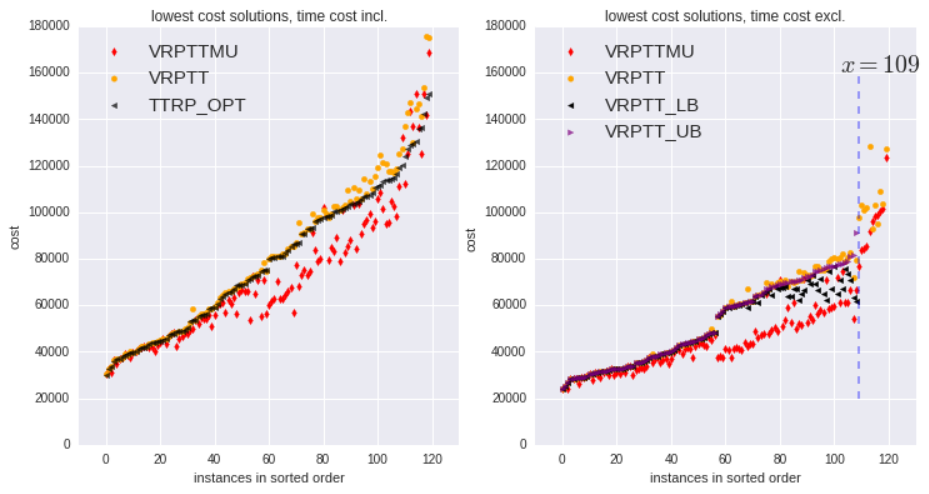
\includegraphics[width=1.3\textwidth]{img/results_1fig.png}}
   \caption{
   The lowest cost found by the VNS for each instance with the available bounds.
   The left plot excludes time cost.
   Its instances are sorted such that the values of TTRP\_OPT increase monotonically.
   The plot on the left includes time cost.
   Its instances are sorted such that all 109 known values of VRPTT\_UB increase monotonically. }
   \label{fig:single_unload}
 \end{figure}


 \setlength\LTleft{-1.3in}
 \setlength\LTright{-1in}
 % \noindent\makebox[]\linewidth]{
 \begin{longtable}{lrrcrrcrr}
   % \\
   \newpage
 \toprule
 % & \multicolumn{2}{c}{time costs included} & \phantom{a}& \multicolumn{4}{c}{excluding time costs} \\
 & \multicolumn{2}{c}{TTRP\_OPT, time cost incl.} & \phantom{a}& %\multicolumn{4}{c}{excluding time costs} \\
 \multicolumn{2}{c}{VRPTT\_LB, time cost excl.}&\phantom{a} & \multicolumn{2}{c}{VRPTT\_UB, time cost excl.} \\
 \cmidrule{2-3} \cmidrule{5-6} \cmidrule{8-9}
  &  VRPTT &  VRPTTMU &&  VRPTT &  VRPTTMU & & VRPTT &  VRPTTMU \\
 \midrule
 %
 2 customers \\
 \cmidrule{1-1}
 count &                30.0 &                  30.0 &&                 30.0 &                   30.0 &&                 30.0 &                   30.0 \\
 mean  &                 0.0 &                  -3.5 &&                 -0.0 &                   -4.5 &&                 -0.0 &                   -4.5 \\
 std   &                 0.6 &                   4.9 &&                  0.1 &                    4.8 &&                  0.1 &                    4.8 \\
 min   &                -1.3 &                 -17.6 &&                 -0.3 &                  -16.0 &&                 -0.3 &                  -16.0 \\
 % 25\%   &                -0.7 &                  -5.7 &&                 -0.0 &                   -8.1 &&                 -0.0 &                   -8.1 \\
 % 50\%   &                 0.4 &                  -1.1 &&                  0.0 &                   -2.3 &&                  0.0 &                   -2.3 \\
 % 75\%   &                 0.4 &                   0.4 &&                  0.0 &                    0.0 &&                  0.0 &                    0.0 \\
 max   &                 0.6 &                   0.6 &&                  0.0 &                    0.0 &&                  0.0 &                    0.0 \\
 \\
 %
 4 customers \\
 \cmidrule{1-1}
 count &                30.0 &                  30.0 &&                 30.0 &                   30.0 &&                 30.0 &                   30.0 \\
 mean  &                 0.7 &                 -10.5 &&                  0.1 &                  -13.8 &&                  0.1 &                  -13.8 \\
 std   &                 1.6 &                  10.1 &&                  0.8 &                   12.8 &&                  0.8 &                   12.8 \\
 min   &                -0.8 &                 -34.2 &&                 -0.4 &                  -37.0 &&                 -0.4 &                  -37.0 \\
 % 25\%   &                 0.4 &                 -21.0 &&                 -0.1 &                  -29.4 &&                 -0.1 &                  -29.4 \\
 % 50\%   &                 0.5 &                  -5.4 &&                 -0.1 &                   -7.0 &&                 -0.1 &                   -7.0 \\
 % 75\%   &                 0.7 &                  -3.2 &&                  0.0 &                   -4.0 &&                  0.0 &                   -4.0 \\
 max   &                 9.0 &                   0.6 &&                  3.6 &                    0.0 &&                  3.6 &                    0.0 \\
 % \pagebreak
 \\
 6 customers\\
 \cmidrule{1-1}
 count &                30.0 &                  30.0 &&                 30.0 &                   30.0 &&                 30.0 &                   30.0 \\
 mean  &                 1.5 &                 -12.9 &&                  3.3 &                  -18.3 &&                  1.0 &                  -20.0 \\
 std   &                 2.3 &                   7.5 &&                  4.3 &                   10.6 &&                  2.0 &                   10.7 \\
 min   &                -0.5 &                 -24.5 &&                 -0.2 &                  -32.9 &&                 -0.4 &                  -32.9 \\
 % 25\%   &                 0.2 &                 -19.4 &&                 -0.0 &                  -27.1 &&                 -0.0 &                  -28.2 \\
 % 50\%   &                 0.7 &                 -13.0 &&                  1.4 &                  -20.6 &&                 -0.0 &                  -23.8 \\
 % 75\%   &                 1.9 &                  -7.5 &&                  5.0 &                   -7.5 &&                  1.2 &                   -7.5 \\
 max   &                 9.5 &                   4.7 &&                 15.8 &                    5.0 &&                  9.6 &                    2.5 \\
 \\
 8 customers \\
 \cmidrule{1-1}
 count &                30.0 &                  30.0 &&                 19.0 &                   19.0 &&                 19.0 &                   19.0 \\
 mean  &                 6.2 &                  -5.2 &&                 13.5 &                   -9.2 &&                  0.6 &                  -19.7 \\
 std   &                 4.8 &                   9.9 &&                  7.4 &                   12.9 &&                  5.0 &                    9.2 \\
 min   &                 0.5 &                 -19.0 &&                  2.9 &                  -25.4 &&                -12.6 &                  -33.3 \\
 % 25\%   &                 2.4 &                 -13.9 &&                  7.1 &                  -18.8 &&                 -0.2 &                  -26.7 \\
 % 50\%   &                 5.9 &                  -6.0 &&                 13.0 &                  -13.8 &&                  1.7 &                  -23.0 \\
 % 75\%   &                 8.0 &                   0.4 &&                 19.7 &                    0.4 &&                  3.6 &                  -14.2 \\
 max   &                17.9 &                  15.8 &&                 28.8 &                   13.3 &&                  5.5 &                   -0.8 \\
 \bottomrule
 \\
 \caption{Statistic per instance size of the gaps between the available bounds and the lowest cost solutions found by the VNS for the VRPTT and VRPTTMU.
}
 \label{tab:gaps}
 \end{longtable}


\subsubsection{VRPTT}

% point 0: probably point 1, one of the brst solutions used trailer sharing. Give simple example with same parameters that does result in optimal solution with trailer sharing. Also critisize why this set should not be used for vrptt.
% point 1: differnce becuase of rounding; see smaller instances up to 4 customers is optimal value.. high prob of having found optimal value.  difference small. Although I followed the described rounding method I have not been able to find exactly the same values. The differences that are present are due to rounding errors. See smaller instances. average gap 0 . Perhpas mixing minutes hours and differnt metohds of rounding
% point 2: weird that vrptt always higher than ttrp.
% point 3: $ttrp < vrptt$ becuase bad algo or becuase bad instance. probably latter since vrptt not higher than vrptt\_UB.
% ALSO: use the figure to make point that follows:
%  See gap wrt to ub vrptt notime compared to gap ttrp for each instance. Are there any instances where there is a high gap with vrptt but small gap with ttrp. If so, there might be evidence that htat is a instance where sharing could be beneficial.
% point 4: examples (in txext) of instances that would have benefited from trailer sharing.\\

%from here ------------------------------------------------
In Table \ref{tab:gaps} we see that for one of the instances with two customers the VNS found a solution for the VRPTT that has a gap of -0.3 \% with the lower bound of the VRPTT, which should not be possible.
For instances with only two customers, where the probability of the VNS finding the optimal solution is the greatest, the mean and the standard deviation of the gap with the optimal value of the VRPTT is 0.0 \% and 0.1 \% respectively and with the optimal value of the TTRP 0.0 \% and 0.6 \% respectively.
The reason for this error is unknown, but at least there is evidence that the mean of the error is zero. \\


Surprisingly, for none of the instances did the best solution use trailer sharing.
This is the reason that in Figure \ref{fig:single_unload} none of the values found by the VNS are significantly lower than the optimal values of the TTRP.
All negative gaps between the values found by the VNS for the VRPTT and the optimal value of the TTRP must thus be attributed to the aforementioned error and not to the benefit of being able to share trailers. \\

Since the results for the VRPTT described in \cite{drexl2014bandc} exclude time related costs and the results for the TTRP described in \cite{drexl2011branch} include time related costs, no conclusions can be drawn about whether sharing trailers leads to solutions with lower costs on these instances based on these results alone.
Only an indirect comparison of these values can be made by using the results found by the VNS.
If sharing trailers leads  to lower cost solutions on these instances,  there may be many instances for which the gap with the upper bound of the VRPTT is significanlty greater than the gap with the optimal value of the TTRP.
In Figure  \ref{fig:gapvsgap} the gap with respect to the optimal value of the TTRP is  plotted against the gaps with respect to the bounds of the VRPTT for each instance.
The figure does not support the conclusion that trailer sharing leads to significantly lower costs on these instances.
In Table \ref{tab:gaps} we see that the mean gaps for instances with two, four, six and eight customers of the VRPTT with respect to the lower bound of the VRPTT  are 0.0, 0.1, 3.3 and 13.5 \% respectively and with respect to the upper bound 0.0, 0.1, 1.0, 0.6 \% respectively.
Therefore, the benefit of sharing trailers can not be ruled out, but can not be shown to be definitely present either.

\begin{figure}[!ht]
  \centering
    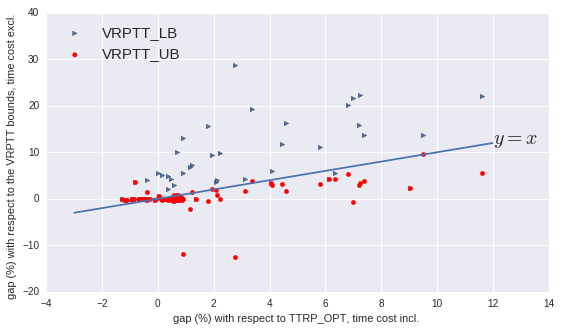
\includegraphics[width=1.0\textwidth]{img/gapvsgap.png}
  \caption{For each instance the gap with respect to the TTRP optimum against the gap with respect to the bounds of the VRPTT. }
  \label{fig:gapvsgap}
\end{figure}


The VNS was able to find solutions for all instances including the eleven instances for which no VRPTT bounds were available.


%
%
%
% a
% Surprisingly, for each instance the best found solution did not use trailer sharing.
% This is reflected in Table \ref{tab:gaps} we see that on the instances
% In Figure \ref{fig:single_unload}
% we see that for all instances the TTRP\_OPT is lower than or equal to the solutions found for the VRPTT.  This is unexpected, since we strange since it is expected that
%
% none of the instances  could our method find a solution that has lower costs than the optimal solution of the TTRP. On average our solution with the lowest cost is $2.1 \%$ more expensive than the optimal solution of the TTRP. Detailed results can be found in Appendix \ref{sec:appendix} This is surprising because one would expect that by sharing trailers between lorries, cost could be reduced. There are two posssiblities.
%  Either on these instances sharing trailers does not reduce costs, or our method could not find those solutions. \\
%
%  When we look at the results in Figure \ref{fig:single_unload} that exclude time related costs we see that for many instances no bounds are known. Our method does find solution for all instances. Our best solution is on average $3.3 \%$ more expensive than the lower bound and $0.4 \% $ more expensive than the upper bound. This gives reason to doubt whether being able to share trailer can reduce costs on these instances.


 \subsubsection{VRPTTMU}

The difference between the VRPTT and the VRPTTMU is that the latter allows lorries to do multiple trips by allowing it to visit the depot multiple times to couple a trailer, decouple a trailer or unload whereas the former does not.
In Figure \ref{fig:single_unload} we can see that for many instances the VNS finds solutions with significantly lower costs than than the TTRP and the VRPTT.
This is not surprising since in some instances less vehicles can be used, which results in less fixed costs.
The instances have such nonrestrictive time windows that one lorry can visit many customers interleaved with depot visits. \\

In Table \ref{tab:gaps} we see that for instances with two, four, six and eight customers the mean gaps with respect to the optima of the TTRP are -3.5, -10.5, -12.9 and -5.2 respectively and with respect to the lower bounds of the VRPTT -4.5, -13.8, -18.3 and -9.2 \% respectively.
This indicates that significant cost reductions can be achieved by allowing lorries to do multiple trips.
For each instance the VNS found a solution to the VRPTTMU. \\

\begin{figure}[!ht]
  \centering
    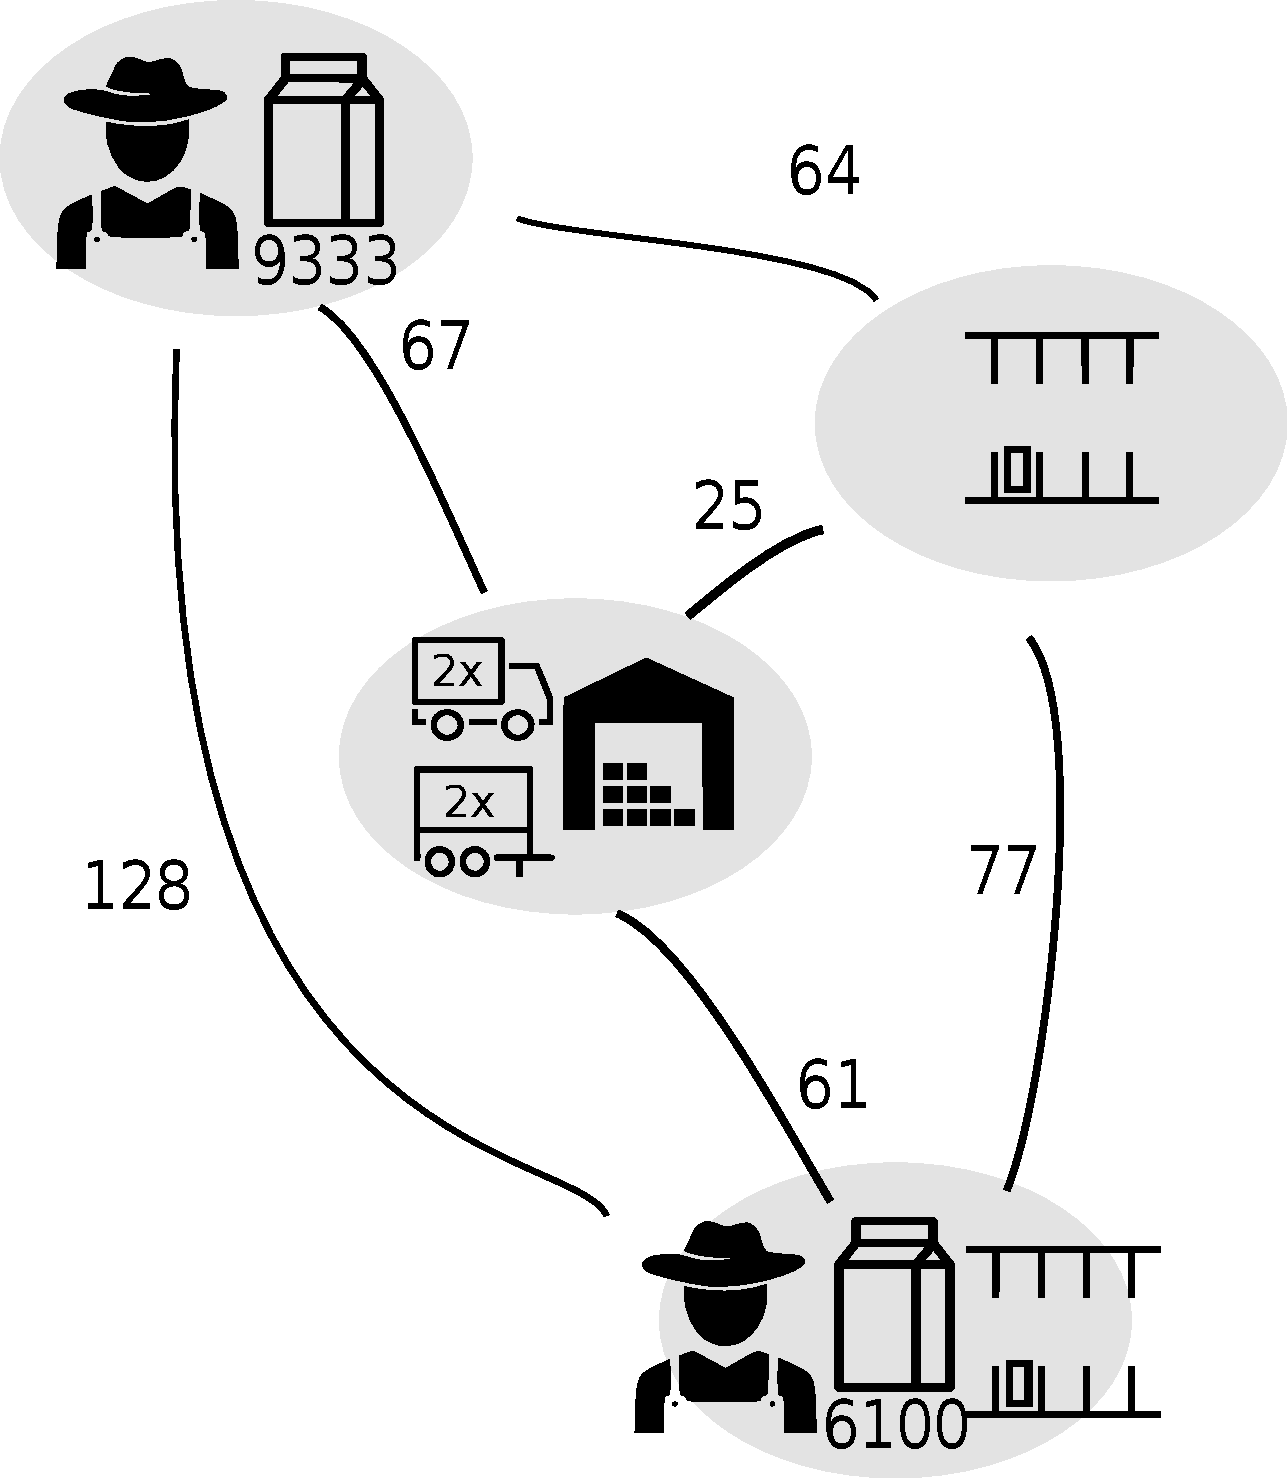
\includegraphics[width=.8\textwidth]{img/1_1_1_4.pdf}
  \caption{Instance $1\_1\_1\_4$ which consist of a depot, a lorry customer, a trailer customer and a pure transshipment location. The distance is in kilometers and the numbers at the customers' is the amount of their supply. The fleet consists of one of each of the vehicles described in Table \ref{tab:vehpar}. }
  \label{fig:instance}
\end{figure}

An example of the benefits of allowing lorries to do multiple trips is given in Figure  \ref{fig:instance}. It illustrates one of the instances with two customers. The fleet consist of one of each of the vehicles described in Table \ref{tab:vehpar}. There is a lorry customer with a supply of 9333 units, a trailer customer with a supply of 6100 units and a pure transshipment location. The time window of each location is the interval [0 , 1320] minutes hence there is enough time for one lorry to visit both customers and collect their supplies.
The sum of the customer supplies is equal to 15433 which is bigger than the capacity of either lorry.
If the lorry is allowed to do multiple trips, it can unload at the depot between visiting the customers.
If this is not allowed, the cheapest solution is to use a trailer.
The fixed cost of this trailer will need to be paid together with its distance related costs.
In Appendix \ref{sec:gaps} we can see that allowing lorries to do multiple trips leads to a gap of -13.8 \% with respect to the optimal value of the TTRP including time costs and -12.5 \% with respect to the optimal value of the VRPTT excluding time costs for this instance.

 % \begin{figure}[h]
 %    %  \makebox[\textwidth][r]{\includegraphics[width=1.2\textwidth]{img/results_multiple_unload.png}}%
 %  %  \centering
 %  % \includegraphics{...}}
 %  % \hspace*{-1.5in}
 %  % \centerline{\includegraphics{...}}
 %     \includegraphics[width=1.\textwidth]{img/results_multiple_unload.png}
 %   \caption{The lowest found costs for the VRPTT with and without time related costs are plotted. Bounds for the TTRP with time related costs and bounds for  the VRPTT without time related costs are given.  Constraint \eqref{con:extra} does not hold. The instances are ordered for a better presentation. }
 %   \label{fig:single_unload}
 % \end{figure}


%  In Figure \ref{fig:single_unload} we see the same bounds, but this time our results represent the best found values without constraint (\ref{con:extra}). For all instances feasible solution could be found. Being able to unload multiple times has significantly reduced costs. When time related costs are included the average gap between  our best solution, and the optimal solution of the TTRP is $ -8.0\%$.
%
% If we exclude time related costs the average gap between the lower (higher) bound and our best solution is $ -11.7\% (-14.0\%)$ .
%
%
%
% %
%
%
%
%
%
%
% \subsection{usefulness multi unload}
% A simple example that illustrates the advantage of being able to unload multiple times is shown in Figure \ref{fig:instance}



% The depot has two available lorries and two available trailers. There are two customers that lie far apart. The vehicles have a speed of 65 kilometers per hour. The time windows of the locations start at 0:00 hours and end at 20:00 hours, so there is more than enough time for a lorry to visit both customers. One lorry has a capacity of 10000 and the other has a capacity of 15000. One trailer has a capacity of 10000 and the other has a capacity of 15000. If constraint (\ref{con:extra}) holds, either two lorries , or a lorry and a trailer have to be used. If the constraint is removed, the cheapest lorry can be used to visit both customers without using a trailer by unloading at the depot before going to the second customer.
%





% % \usepackage{booktabs}
% \newcommand{\ra}[1]{\renewcommand{\arraystretch}{#1}}
% \begin{table*}\centering
% \ra{1.3}
% \begin{tabular}{@{}rrrrcrrrcrrr@{}}\toprule
% & \multicolumn{3}{c}{$w = 8$} & \phantom{abc}& \multicolumn{3}{c}{$w = 16$} &
% \phantom{abc} & \multicolumn{3}{c}{$w = 32$}\\
% \cmidrule{2-4} \cmidrule{6-8} \cmidrule{10-12}
% & $t=0$ & $t=1$ & $t=2$ && $t=0$ & $t=1$ & $t=2$ && $t=0$ & $t=1$ & $t=2$\\ \midrule
% $dir=1$\\
% $c$ & 0.0790 & 0.1692 & 0.2945 && 0.3670 & 0.7187 & 3.1815 && -1.0032 & -1.7104 & -21.7969\\
% $c$ & -0.8651& 50.0476& 5.9384&& -9.0714& 297.0923& 46.2143&& 4.3590& 34.5809& 76.9167\\
% $c$ & 124.2756& -50.9612& -14.2721&& 128.2265& -630.5455& -381.0930&& -121.0518& -137.1210& -220.2500\\
% $dir=0$\\
% $c$ & 0.0357& 1.2473& 0.2119&& 0.3593& -0.2755& 2.1764&& -1.2998& -3.8202& -1.2784\\
% $c$ & -17.9048& -37.1111& 8.8591&& -30.7381& -9.5952& -3.0000&& -11.1631& -5.7108& -15.6728\\
% $c$ & 105.5518& 232.1160& -94.7351&& 100.2497& 141.2778& -259.7326&& 52.5745& 10.1098& -140.2130\\
% \bottomrule
% \end{tabular}
% \caption{Caption}
% \end{table*}


% \newpage
% \input{real_values.tex}


% plot here:
% violin plot.
%
% 1 x value for each instance size group.
% left size is for
%
% Give the plot such that I can say:
% we see that our algo does not find results as good as the ttrp algo. This can have 2 reason either they are there but hte algo does not find them, or no better sols exist and therefore they are not found. Looking at the figures, we see that the

% \subsubsection{VRPTT Instances}
% Drexl's instances used in \cite{drexl2014bandc} with up to 8 requests have been used to test the algorithm.
%
% \begin{table}[ht]
% \centering
% \caption{My caption}
% \label{my-label}
% \begin{tabular}{llllll}
% \hline
%                 & Capacity             & Fixed costs & Costs per km & Driving speed & $C_k$ \\ \hline \hline
% Lorry class 1   & 10000              & 180    & 0.65       & 65            & $\{1,2\}$                        \\ \hline
% Lorry class 2   & 15000                & 200    & 0.7        & 65            & $\{1\}$                          \\ \hline
% Trailer class 1 & 10000       & 20     & 0.04       &               &  $\{1,2\}$                          \\ \hline
% Trailer class 2 & 15000          & 25   & 0.04          &               &   $\{1\}$                         \\ \hline
% \end{tabular}
% \end{table}
%
% \todo{add details about parameters}
%
% \subsubsection{TTRP Instances}
% Drexl's instances with up to 25 requests used for the truck-and-trailer routing problem in  \cite{drexl2011branch}.
%
% \subsection{Results}
% In the table below  we can observe \ldots
% \subsection{Usefulness Trailer Sharing}


\newpage
\section{Conclusion}

\label{chap:Discussion and Future Work}

% disqualified data set for testing trailer sharing

% improved ub for some instances excl costs

% define exactly the what method of drexl i tried to follow with regards to time roudning

% are there any instances that i have lower value than ttrp? if so, is that because error or because trailer sharing?

% much smaller than transmission. they have much bigger instances. 24 depots. Perhaps persue ttrp first, after that see if i can extend the model, or postprocess ttrp sols for trailer sharing opportunities


% A few contributions have been made in this thesis:
% \begin{itemize}
%   \item Trailers have their own maximum speed such that it is possible that a lorry's maximum speed is higher without a trailer than with a trailer.
%   \item The manner in which the model represents load transfers has been simplified.
%   \item The VRPTT has been remodeled such that it can be extended to the VRPTTMU by only removing one set of constraints and by adding a certain type of trailer to the instances that does not have   influence on the best solutions of the VRPTT.
%   \item A variable neighborhood search heuristic has been presented and implemented which found solutions for the VRPTT and the VRPTTMU  for all instances with up to eight customers in minutes.
%   \item The results of this heuristic were used to show that it is not at all clear that the instances used in this thesis are suitable to show the benefits of trailer sharing.
%   % \item An example of an instance that does benefit from trailer sharing has been given.
%
% \end{itemize}

%
% The VRPTT has been remodeled such that it can be extended to the VRPTTMU by only removing one set of constraints and by adding a certain type of trailer to the instances that does not have   influence on the best solutions of the VRPTT.
A few contributions have been made in this thesis.
Trailers have their own maximum speed such that it is possible that a lorry's maximum speed is higher without a trailer than with a trailer.
The manner in which the model represents load transfers has been simplified by removing the need for vertices only dedicated to transfering load.
The VRPTT has been remodeled such that it can be extended to the VRPTTMU by only removing one set of constraints and by adding a certain type of trailer to the instances that does not have   influence on the best solutions of the VRPTT.
The VRPTTMU is able to represent the situation where lorries visit the depot multiple times without ending their path to either couple or decouple a trailer or to unload their load.
This allows lorries to take multiple trips which resulted in significantly decreased costs on many test instances.
A variable neighborhood search heuristic has been presented and implemented which found solutions for the VRPTT and the VRPTTMU  for all instances with up to eight customers in minutes.
The objective function of the VRPTT has been extended such that besides the fixed costs and the distance related costs, the  objective function is also a function of the time related costs.
This allowed a comparison with results to the TTRP for the first time, which showed that it is not at all clear that the instances used in this thesis are suitable to show the benefits of trailer sharing.
Perhaps these benefits become more apparent as the size of the problem instance grows.
% \item An example of an instance that does benefit from trailer sharing has been given.
\\


% Powerful algorithms for solving the VRPTT do not exist yet \cite{drexl2014bandc}.
% Stochastic optimization methods and/or heuristics may offer solutions in cases where solving problems exactly is too slow.
% Developing such an algorithm is therefore the most logical first step towards solving TransMission's problem. This task is the scope of this thesis. The optimization method will be a simplified version of the ALNS, namely a variable neighborhood search (VNS). The ALNS  has shown promising results on large instances in \cite{masson2013adaptive}.\\

The aim of this thesis was to develop a heuristic that can handle larger instances than exact methods and that can be extended such that it can be used to develop a solution for  TransMission's problem.
This goal has been achieved with the VNS heuristic.
The heuristic found in a short period of time reasonably good solutions for all tested instances, even for the instances for which the exact method could not find a solution.
An extension of the model that reduces costs has already been demonstrated by allowing lorries to unload multiple times.
Furthermore, since the heuristic is fairly simple and unoptimized, there is reason to believe that it can be optimized for better performance. \\


Before the results of this thesis can be used by TransMission to produce transport plans some work still has to be done.
The model has to be extended such that it supports multiple commodities, multiple depots and split deliveries.
% Futhermore, it has to perform well the optimization method has to be tested on and optimized for much larger instances.

% Extened the vprtt.
% raised doubts about validity of instances.
% a variable neighborhood search hurisitic is implemented to solve the problems.
%
% --------------------------------------------
%
% modelling of load transfer
% A few additions have been made to the VRPTT model.
% The  VRPTT model has been extended in a realistic way  that makes solutions with lower costs feasible by allowing lorries to unload multiple times at the depot.
% The model has also been simplified by removing vertices specific for load transfers from the model.
%
% TODO: some indication that the instances used in this thesis are not well suited to show the benefits of trailer sharing.
% On the other hand, perhaps sharing trailers becomes more advantageous as the size of the instance increases.
%
% These instances were very suitable  to demonstrate the advantage of a lorry being able to visit the depot multiple times, either to decouple or couple a truck or to unload.
%
%
% Furthermore, a simple search heuristic was presented for the VRPTT which performs reasonably well.
% It was able to find feasible solution for all instances within a short running time.

\section{Future Work}
\label{chap:future-work}
% An obvious improvement that can be made to the model is to reduce the amount of symmetry in the model.
% In the current representation of a solution, multiple representations can map to the same solution.
% This can be alleviated by adding constraints which remove that symmetry.
% Another improvement is to remove the need to create $\eta$ transshipment vertex pairs for each transshipment location, but to generate them when needed by the optimization method. \\

There are improvements that can be made to the model:
\begin{itemize}
\item The amount of symmetry in the model could be reduced by adding certain constraint to the model.
In the current representation of a solution, multiple representations can map to the same solution.
\item The need to create $\eta$ transshipment vertex pairs for each transshipment location instead of generating them when needed by the optimization method can be removed.
\end{itemize}

There are ways that the model can be extended:
\begin{itemize}
  \item The model can be extended from a vehicle routing problem to a pickup and delivery problem.
  \item The model can be extended such that it can represent a set of customers that can change during the time horizon.
  \item The model can be extended such that it supports multiple depots.
  \item The model can be extended such that it can model split deliveries.
  \item The model can be extended such that the maximum amount of a customer's supply is  unrelated to the capacity of the vehicles.
%   \item The model can be extended such that there are less restrictions on the availabel vehicles.
\end{itemize}

There are improvements that can be made to the optimization method:
\begin{itemize}
\item More constraints could be turned into soft constraints like the precedence of decoupling a trailer over coupling a trailer at a transshipment vertex.
\item A solution can be decomposed into several sub-solutions which are independent of each other with respect to each others load and time table.
The current method recalculates the sub-solutions for each new solution even if the sub-solutions have already been seen before in other solutions.
This can be resolved by caching the sub-solutions of solutions.
\item New operators can be developed to speed up the search heuristic.
\item The parameters used by the optimization method can be tuned by performing a  hyperparameter optimization.
\item The time table algorithm can be improved for the VRPTTMU which potentially leads to a reduction of trailers' time related cost.
\item A probabilistic datastructure like a bloom filter can be used for the tabu table to reduce its memory consumption.
\item The method could be adapted such that it can be executed in parallel.
\end{itemize}

There are improvements that can be made to the testing method:
\begin{itemize}
\item The influence that neighborhood operators have on the results could be tested.
\item The influence that turning a constraint into a soft constraint has on the results could be tested.
\item The method can be tested for more iterations and on larger instances.
\item Different types of instances could be used to test the relation between instance characteristics and the benefits of trailer sharing.
\end{itemize}




\begin{comment}

\begin{itemize}
\item futher reduction of time -dependent trailer costs in VRPTTMU by better tiem table scheduling
\item when lorry visits a trailer customer with trailer and wants to uncouple, remove state whether decoupling happens before supply collection or after. Source of symmetry.
\item replace current tabu set with something like a bloom filter. which has better memory and speed characteristics and only has a small probability of but small probability of false positive which will lead you to know evaluate a random solution.
\item reformulate the model such that y is not necessary. All the trailer paths and assginemtnes can already be deduced from x.
\item instead of generating all logic equiv and storing them, reduce back to canonical form. First check for the found form, then reduce and check
\item have cash for time dependent paths.
\item some more sophisticated priority functions that for example also weights which operator is applied.
\item decompose vehicle assignment from paths searching.
\item decompose path construction from grouping customers, i.e. a path or multiple paths with possibly use of trailers is  independently planned for group of customers .
\item currently start and stop time of lrry is equal to start and stop time of depot. In future i could give individual times per lorry.
\item Let lorries start later if that is more optimal instead of starting each lorry at the start of its time window.
\item instead of generating all identicals, reduce to unique sort, using some kind of topological sort and prove that it is unique.
\item use some form of memozation. For example, cost of an indepent vehicle route, can be looked up before evaluated.
\item add actions that can evaluate a neighboring solution without having to calculate a full evaluation. For example in case you know the change does not impact any other route. And you can efficiently calculate delta time and delta distance. Much more computationally efficient.
\item add some initial solution method to speed up computation.
\item add new search methods like 3-opt and hyperopt
\item More efficient method for choosing action, in particular reducing regret. Perhaps even using current state of instead of past results.
\item Allow vehicles to unload at the depot without ending their route.
\item Dynamic allocation of vertices to couple and uncouple pairs. Now I have to statically allocate them on forehand. I can use this same method to dynamically allocate unload locations at the depots. Now a vertex is tied to an operation and a location. Time, cap and lorry are assigned to it. Would be nice if operation and location were also assignable.
\item Extend the model to pickup-and-delivery
\item Further explore adding extra trailers to instances that serve as extra unload places for lorries. Give them huge distance costs such that won't be used for anywhere else than on the depot.

\item Define an extension of the Generalized Assignment Problem that can be used for vehicle assignment. I nput is a certain set of paths, output is the cheapest assignment of vehicles to these paths that does not violate any time constraints of load constraints. There are no load costs. Whether there is a way to put the load in available vehicles is possible to solve with constraint solver. Do I even need maxflow? The way load flows from lorry to trailer can be determined with a few extra vars in the integer program. Time costs can be expressed in terms of the vehicle assignment. This can be used to speed up the search (either compute for each in consume or add as one of the actions), or to dramatically reduce the solution space. The solution space now only represents trailer start and end vertices, transshipment couple and decouple vertices and supply collection vertices.
\item explore whether I cannot reduce the load problem to a much smaller problem. A constraint satisfaction problem. The amount of unknown variables is equal to the amount of trailer segments, since the only unknowns are how much load a lorry transfers to a trailer during a segment.
\item Given a paths can I express load as constraint satisfaction and time as symbolic function such that both can be efficiently computed for different vehicle assignments.
\item Just like the last item see if I can do more with symbolic programming and constraint satisfation. Time table can be expressed in terms of vehicle assingment. load table constraint satisfaction problem.
\item include some notion of progress, e.g. currently at iteration 1000 of 2000 to guide how exploration vs exploitation. Hence the pq sorting key (-> search direction) will depend not only on task_features but aslo  on current iteration.
\item more intelligent chooser for which task to execute, perhaps use rl
\item process task in parallel. Perhaps using aws lambda or on gpu using opencl
\item Insert more types of actions, e.g. like 2-opt
\item Futher reduce search space s.t. it does not matter in which order you uncouple, i.e. first uncouple at trailer customer then supply collect or first supply collect then trailer uncouple can be made the same, if it does not matter for the solution. Problem:: it may matter for solutions that can be made out of this solution. Soltuion perhaps?, introduce 2-opt.
\item Perhaps use first smaller problem ttrp than remove constraint st trailers can be shared to solve vrptt with bigger solution space, then remove another constraint s.t. lorry paths  dont have to end if they arrive at depot. Hence three levels of problem. Do this by adding actions.
\item express solutions a bit different such that  I don't have to generate all duplicates, but such that there is only 1 way to express a functional equivalent solution by not expressing which vehicle, and which trailer and which .

\end{itemize}

\end{comment}


\newpage
%
% % % \usepackage{booktabs}
% \newcommand{\ra}[1]{\renewcommand{\arraystretch}{#1}}
% \begin{table*}\centering
%
% % \resizebox{100}
% \begin{tabular}{@{}rrrrcrrrcrrr@{}}\toprule
% & \multicolumn{3}{c}{$w = 8$} & \phantom{abc}& \multicolumn{3}{c}{$w = 16$} &
% \phantom{abc} & \multicolumn{3}{c}{$w = 32$}\\
% \cmidrule{2-4} \cmidrule{6-8} \cmidrule{10-12}
% & $t=0$ & $t=1$ & $t=2$ && $t=0$ & $t=1$ & $t=2$ && $t=0$ & $t=1$ & $t=2$\\ \midrule
% $dir=1$\\
% $c$ & 0.0790 & 0.1692 & 0.2945 && 0.3670 & 0.7187 & 3.1815 && -1.0032 & -1.7104 & -21.7969\\
% $c$ & -0.8651& 50.0476& 5.9384&& -9.0714& 297.0923& 46.2143&& 4.3590& 34.5809& 76.9167\\
% $c$ & 124.2756& -50.9612& -14.2721&& 128.2265& -630.5455& -381.0930&& -121.0518& -137.1210& -220.2500\\
% $dir=0$\\
% $c$ & 0.0357& 1.2473& 0.2119&& 0.3593& -0.2755& 2.1764&& -1.2998& -3.8202& -1.2784\\
% $c$ & -17.9048& -37.1111& 8.8591&& -30.7381& -9.5952& -3.0000&& -11.1631& -5.7108& -15.6728\\
% $c$ & 105.5518& 232.1160& -94.7351&& 100.2497& 141.2778& -259.7326&& 52.5745& 10.1098& -140.2130\\
% \bottomrule
% \end{tabular}
% \caption{Caption}
% \end{table*}



%
% \setlength\LTleft{-1in}
% \setlength\LTright{-1in}
% % \begin{longtable}{@{\extracolsep{\fill}}*{13}{|r}|@{}}
% %
% %
% %
% \begin{longtable}{lrrrcrrrr}
% \toprule
% %
% & \multicolumn{3}{c}{including time costs} & \phantom{a}& \multicolumn{4}{c}{excluding time costs} \\
% \cmidrule{2-4} \cmidrule{6-9}
% %
% %
% % & \multicolumn{2}{c}{VRPTT} &\multicolumn{2}{c}{VRPTTMU} &
% % \phantom{abc} & \multicolumn{2}{c}{VRPTT} &\multicolumn{2}{c}{VRPTTMU} \\
% %
% instance &  VRPTT &  VRPTTMU &  OPT\_TTRP &&  VRPTT &  VRPTTMU &  LB\_VRPTT &  UB\_VRPTT \\
% %




\appendix

\section{Symbols and Abbreviations}


Many symbols and abbreviations are used throughout this thesis.
They are enumerated with their meaning in Table \ref{tab:symbols}.

% \begin{}[!h]
% \centering
% \caption{Symbols and abbreviations with their meanings.}
% \label{tab:symbols}
\setlength\LTleft{-1.1in}
\setlength\LTright{-2in}
\begin{longtable}{ll}

\toprule
Symbol       & Meaning       \\ \midrule \endhead
VRP & The vehicle routing problem. \\
RVRP & The rich vehicle routing problem. \\
VRPMS & The vehicle routin problem with multiple synchronization constraints. \\
VRPTT & The vehicle routing problem with trailers and transshipments. \\
VRPTTMU & The vehicle routing problem with trailers, transshipments and multiple unloads. \\

\includegraphics[width=.04\textwidth]{img/lorry_icon.pdf} & The  lorry icon. \\

\includegraphics[width=.04\textwidth]{img/trailer_icon.pdf} & The trailer icon. \\

\includegraphics[width=.04\textwidth]{img/couple_vertex.pdf} & The transshipment couple vertex icon. \\

\includegraphics[width=.04\textwidth]{img/decouple_vertex.pdf} & The transshipment decouple vertex icon. \\

\includegraphics[width=.04\textwidth]{img/supply_vertex.pdf} & The  supply collection vertex icon.\\

\includegraphics[width=.04\textwidth]{img/time-window_icon.pdf} & The time window icon. \\

\includegraphics[width=.04\textwidth]{img/vehicle_start.pdf} & The start of vehicle path vertex icon. \\

\includegraphics[width=.04\textwidth]{img/vehicle_end.pdf} & The end of vehicle path vertex icon.\\

\includegraphics[width=.04\textwidth]{img/transshipment_location_icon.pdf} & The transshipment location icon.\\

\includegraphics[width=.04\textwidth]{img/customer_location_icon.pdf} & The customer icon. \\

\includegraphics[width=.04\textwidth]{img/depot_location_icon.pdf} & The depot icon.\\

\includegraphics[width=.04\textwidth]{img/super_source_icon.pdf} & The supersource vertex icon. \\

\includegraphics[width=.04\textwidth]{img/super_sink_icon.pdf} & The supersink vertex icon.\\
$\mathcal L$ & The set of locations. \\
$\mathcal D$ & The mapping from a pair of locations to the distance between them. \\
$\mathcal F$ & The set of vehicles in the fleet. \\
$\mathcal L^{\rm types}$ & The set of location types. \\
$locationType_i$ & The location type of location $i$. \\
$\alpha_i$ & The start of the time window of location $i$. \\
$\beta_i$ & The end of the time window of location $i$. \\
$\mathcal L^{\rm customer}$ & The set of customer locations. \\
$locationSupply_i$ & The supply of customer location $i$. \\
$\mathcal F^{\rm types}$ & The set of vehicle types. \\
$\mathcal F^{\rm lorry}$ & The set of vehicle lorries. \\
$\mathcal F^{\rm trailer}$ & The set of trailers. \\
$\mathcal F^{\rm axle-types}$ & The set of axle types of vehicles.\\
$f^{\rm type}_k$ & The vehicle type of  vehicle $k$. \\
$f^{\rm capacity}_k$ & The capacity of vehicle $k$. \\
$f^{\rm fixed}_k$ & The fixed cost of vehicle $k$. \\
$f^{\rm distance}_k$ & The variable distance cost of vehicle $k$ per kilometer. \\
$f^{\rm time}_k$ & The variable time cost of vehicle $k$ per hour. \\
$f^{\rm axle-type}_k$ & The axle type of vehicle $k$. \\
$f^{\rm speed}_k$ & The maximum speed of vehicle $k$ on distances longer than $\phi$. \\
$f^{\rm shortspeed}_k$ & The maximum speed of vehicle $k$ on distances shorter than or equal to $\phi$. \\
$f^{\rm loadspeed}_k$ & The load speed of lorry $k$ in minutes per unit. \\
$\phi$ & The cut-off distance that determines the maximum speed of the vehicles. \\
$\tau^{\rm D}$ & The duration of coupling or decoupling a trailer at the depot in minutes. \\
$\tau^{\rm R}$ & The duration of coupling or decoupling a trailer at a transshipment location in minutes. \\
$\mathcal R^-$ & The set of transshipment decouple vertices. \\
$\mathcal R^+$ & The set of transshipment couple vertices. \\
$\mathcal L^{\rm transshipment}$ & The set of transshipment locations. \\
$r^{j,-}_m$ & The decouple vertex of the $m$th transshipment vertex pair  at transshipment location $j$. \\
$r^{j,+}_m$ & The couple vertex of transshipment vertex pair $m$ at transshipment location $j$. \\
$\eta$ & The amount of transshipment vertex pairs per transshipment location. \\
$\mathcal S$ & The set of the customers' supply collection vertices \\
$s_i$ & the supply collection vertex of customer location $i$. \\
$\mathcal S^{\rm trailer}$ & The set of supply collection vertices of the the trailer customers.  \\
$\mathcal S^{\rm lorry}$ & The set of supply collection vertices of the lorry customers. \\
$\mathcal M^-$ & The set of end vertices of the lorries.\\
$\mathcal M^+$ & The set of start vertices of the lorries. \\
$m^-_k$ & The end vertex of lorry $k$. \\
$m^+_k$ & The start vertex of lorry $k$. \\
$\mathcal N^-$ & The set of end vertices of the trailers.\\
$\mathcal N^+$ & The set of start vertices of the trailers. \\
$n^-_l$ & The end vertex of trailer $l$. \\
$n^+_l$ & The start vertex of trailer $l$. \\
$\mathcal V$ & The union of the set of vehicle start and end vertices, the set of transshipment decouple \\
& and couple vertices and the set of customer supply collection vertices.  \\
$v^{\rm loc} $ & The location of vertex $v$. \\
$\tau^{\rm start}_v $ & The start of vertex $v$'s time window. \\
$\tau^{\rm end}_v $ & The end of vertex $v$'s time window. \\
$\tau^{\rm min} $ & The start of the time horizon. \\
$\tau^{\rm max} $ & The end of the time horizon. \\
$\delta_{u,v} $ & The distance between vertex $u$ and $v$. \\
% $\epsilon^{\phi}_i$ & the set of vertices distanced less than $\phi$ from vertex $i$ \\
$\tau^{\rm travel}_{u,v,k} $ & The travel time of vehicle $k$ between vertices $u$ and $v$.\\
$\tau^{\rm extra}_{u,v,k,l} $ & The extra time it takes for lorry $l$ to traverse edge $(u,v)$ if it is \\
&  coupled with trailer $l$. \\
$travelTime$ & The function that takes as input an edge and a path assignment and returns the amount of time \\
&  it took for vehicles to traverse that edge.\\
$visitationStart$ & The function that takes as input a vertex, a path assignment and a time table and \\
& returns the time at which the the vertex' visitation started. \\
$\mathcal E $ & The set of edges $ \{ (u,v): u,v \in \mathcal V , u \neq v \} $. \\
$\mathcal G $ & The graph $ (\mathcal V, \mathcal E) $. \\
$x^k_{u,v}$ & The binary decision variable that models whether lorry $k$ traverses edge $(u,v)$. \\
$y^{k,l}_{u,v}$ & T`he binary decision variable that models whether lorry $k$ traverses edge $(u,v)$ \\
& whilst coupled to trailer $l$. \\
$t^k_{u,v}$ & The real-valued decision variable that models at which time lorry $k$ finishes traversing edge $(u,v)$. \\
$z^k_{u,v}$ & The real-valued decision variable that models the amount of load with which \\
&   vehicle $k$ traverses edge $(u,v)$. \\
% $ X$ & $ (x^k_{u,v}) \text{ for } k \in  \mathcal F^{\rm lorry}, u,v \in \mathcal V$ \\
% $ Y$ & $ (y^{k,l}_{u,v}) \text{ for } k \in  \mathcal F^{\rm lorry} ,
% \l  \in  \mathcal F^{\rm trailer}, u,v \in \mathcal V$ \\
% $ T $&$ (t^k_{u,v}) $ for $ k \in  \mathcal F^{\rm lorry}, u,v \in \mathcal V$ \\
% $ L $&$ (z^k_{u,v}) $ for $ k \in  \mathcal F, u,v \in \mathcal V$ \\
$C$ & The objective function. \\
$C^{\rm distance}$ & The function that calculates the distance-related costs of a solution. \\
$C^{\rm time}$ & The function that calculates the time-related costs of a solution. \\
$C^{\rm fixed}$ & The function that calculates the fixed costs of a solution. \\
$X$ & The lorries' paths of a solution.  \\
$Y$ & The trailers' paths of a solution.\\
$T$ & The time table of a solution.\\
$L$ & The load table of a solution.\\
$XY$ & The path assignment $(X,Y)$. \\
VNS & The variable neighborhood search . \\
$\omega^{\rm unserved-customer} $ & The penalty for not serving a  customer.  \\
$U^{\rm unserved-customer} $ & The function that calculates the penalty of a solution due to unserved customers. \\
$\omega^{\rm lorry-customer} $ & The penalty for visiting a lorry customer with a trailer. \\
$U^{\rm lorry-customer} $ & The function that calculates the penalty of a solution due to lorry customers visited with trailers. \\
$\omega^{\rm time-window} $ & The penalty per minute for a lorry violating the end of a vertex' time window. \\
$U^{\rm time-window} $ & The function that calculates the penalty of a solution due to violated time windows. \\
$\omega^{\rm capacity-shortage} $ & The penalty per supply unit left uncollected of a visited customer. \\
$U^{\rm capacity-shortage} $ & The function that calculates the penalty of a solution due to uncollected supply of \\
&  visited customers. \\
$U$ & The functional that calculates the penalty of a solution. \\
% $\mathcal O$ & The set of neighborhood operators. \\
$nSamples$ & The amount of path assignments that the operation $merge lorries$ returns. \\
$\mathcal G^{\rm c}$ & The capacity graph $(\mathcal V^{\rm c},\mathcal E^{\rm c})$. \\
$\mathcal V^{\rm c}$ & The set of vertices of the capacity graph $\mathcal G^{\rm c}$. \\
$\mathcal E^{\rm c}$ & The set of edges of the capacity graph $\mathcal G^{\rm c}$.\\
$capacity $ & A mapping from edges in the capacity graph to their capacities. \\
$\mathcal P$ & The set of vertices used to model load transfers to trailers when constructing the load table.  \\
$p_l$ & The vertex used to model load transfers to trailer $l$ when constructing the load table. \\
$source $ & The vertex used as a supersource when constructing the time and load table. \\
$sink $ & The vertex used as a supersink when constructing the time and load table. \\
$f^{\rm c} $ & A mapping that represent the solution to the maximum flow problem on the capacity graph \\
& from the supersource to the supersink.   \\
$|f^{\rm c}| $ & The total amount of customer supply collected. \\
$\mathcal G^{\rm trailer}$ & The graph $(\mathcal V$ used to determine trailers' trailer paths. \\
$trailerPath_l$ & The trailer path of trailer $l$ which is used to determine the load of a trailer during \\
& each edge it traverses. \\
$\mathcal E^{\rm pair}$  & The set of edges that connects each transshipment decouple vertex with the \\
& couple  vertex it is paired with.  \\
$\mathcal E^{\rm used-trailer}$  & The set of edges traversed by any trailer.  \\
$\mathcal V^{\rm precedence}$ & The set of vertices used to model the precedence graph. \\
$\mathcal E^{\rm earliest}$ & The set of edges used to calculate the earliest arrival times. \\
$\mathcal E^{\rm latest}$ & The set of edges used to calculate the latest time at which trailers start can start their paths.  \\
$duration^{\rm earliest}$ & A function that maps from edges to their weights. \\
$duration^{\rm latest}$ & A function that maps from edges to their weights. \\
$duration^{\rm result}$ & A function that maps from edges to their weights. \\
$\mathcal G^{\rm earliest}$ & $(\mathcal V^{\rm precedence},\mathcal E^{\rm earliest},duration^{\rm earliest} )$ \\
$\mathcal G^{\rm latest}$ & $(\mathcal V^{\rm precedence},\mathcal E^{\rm latest},duration^{\rm latest} )$ \\
$\mathcal G^{\rm result}$ & $(\mathcal V^{\rm precedence},\mathcal E^{\rm earliest},duration^{\rm result} )$ \\
$\mathcal V^{\rm start}$ & The set of edges used to model the start of vertex visits in a precedence graph. \\
$\mathcal V^{\rm end}$ & The set of edges used to model the end of vertex visits in a precedence graph. \\
$\mathcal E^{\rm latest-start}$ & The set of edges used to constrain the time at which lorries start their paths. \\
$score$ & The function that calculates the score of a solution, which is the sum of its costs \\
&  and its penalties. \\
$TABU$ & The collection that is used to cache path assignments. \\
$PQ$ & The collection that keeps solutions with unexplored neighborhoods in sorted order. \\
$p$ & The probability that a random item is removed from the $PQ$ instead the one  \\
& with the highest priority. \\
$VRPTT\_UB$ & Upper bounds for the VRPTT excluding time costs. \\
$VRPTT\_LB$ & Lower bounds for the VRPTT excluding time costs. \\
$TTRP\_OPT$ & The optimal values for the TTRP including time costs. \\

% $trailerPath_l$ & the sequence of vertices visited by vehicle $k$ \\
\bottomrule
\caption{Symbols and abbreviations with their meanings.}
\label{tab:symbols}
\end{longtable}


% \begin{figure}[!ht]
%   \centering
%     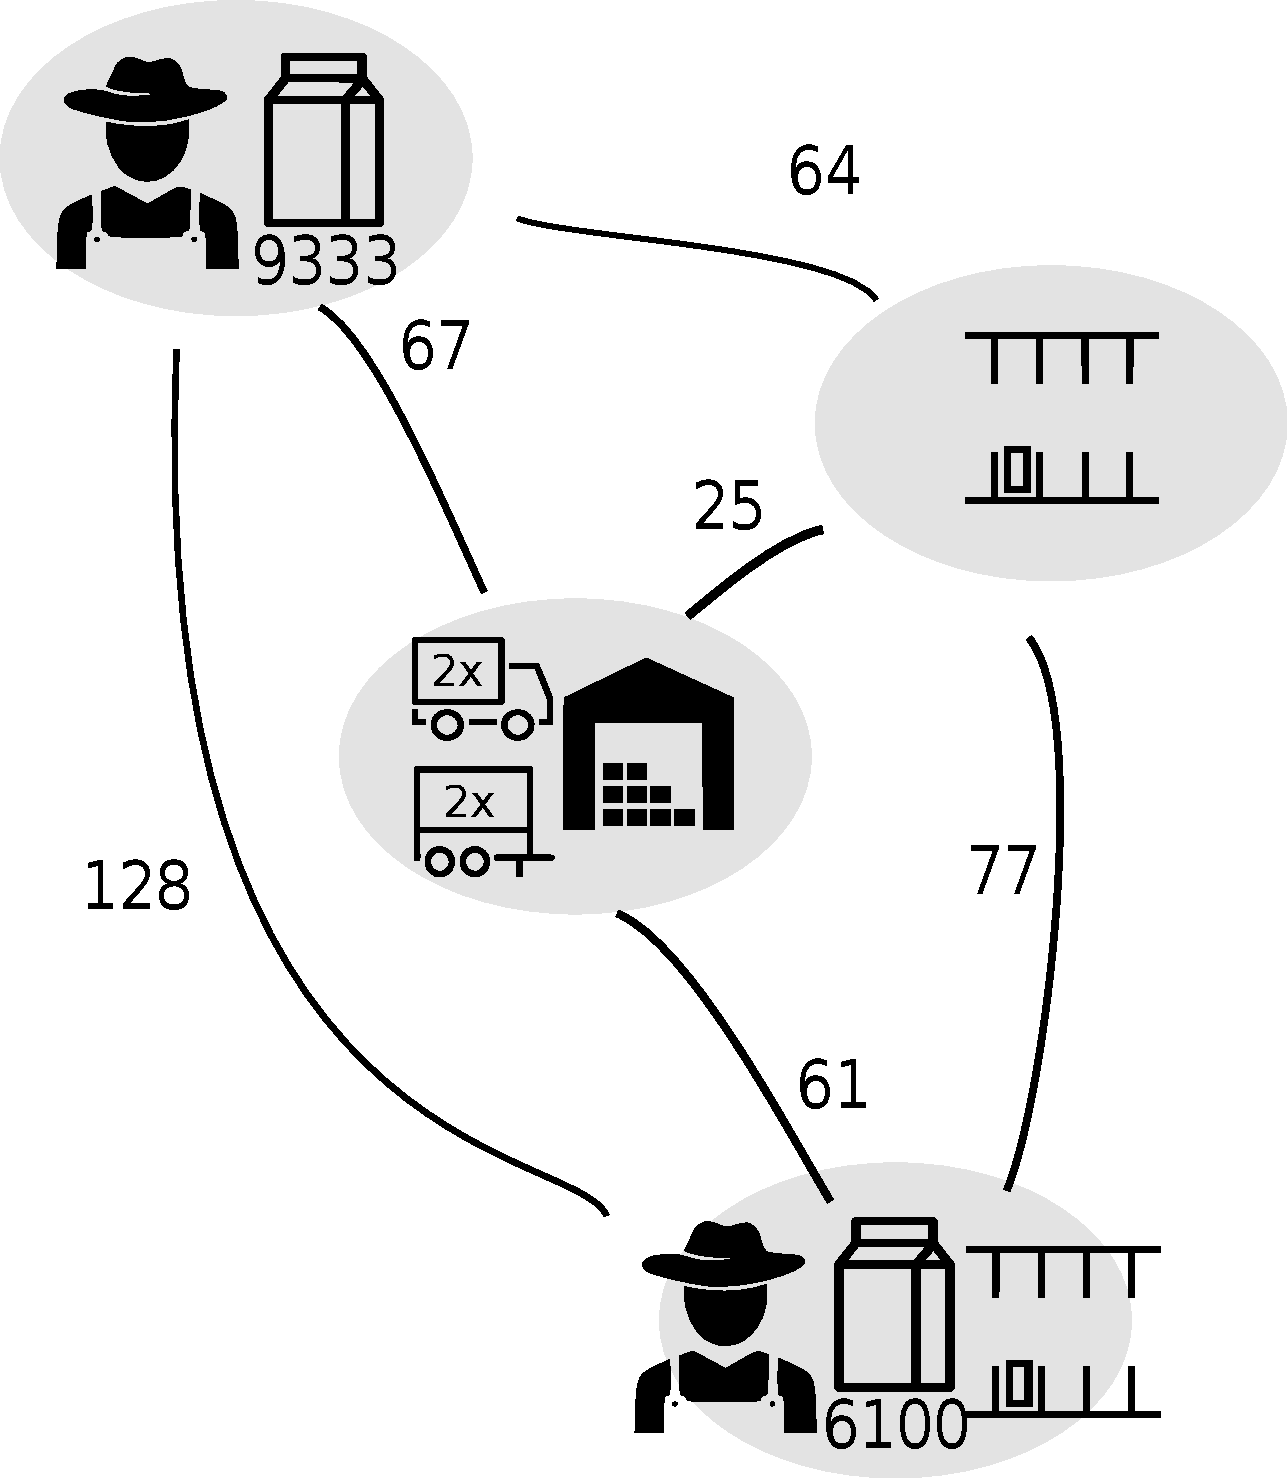
\includegraphics[width=.8\textwidth]{img/1_1_1_4.pdf}
% \end{figure}

\section{Results and Bounds}
\subsection{Nominal Values}
\label{sec:bounds}

Table \ref{tab:nominal} describes for each instance the lowest cost solution found by the VNS for the VRPTT and the VRPTTMU  and  the optimal value for the TTRP provided in \cite{drexl2011branch} which include time costs  and the lower and upper bound of the VRPTT provided in ~\cite{drexl2014bandc} which exclude time costs.




%
\setlength\LTleft{-1in}
\setlength\LTright{-1in}
% \begin{longtable}{@{\extracolsep{\fill}}*{13}{|r}|@{}}
%
%
%
\begin{longtable}{lrrrcrrrr}
\toprule
%
& \multicolumn{3}{c}{including time costs} & \phantom{a}& \multicolumn{4}{c}{excluding time costs} \\
\cmidrule{2-4} \cmidrule{6-9}
%
%
% & \multicolumn{2}{c}{VRPTT} &\multicolumn{2}{c}{VRPTTMU} &
% \phantom{abc} & \multicolumn{2}{c}{VRPTT} &\multicolumn{2}{c}{VRPTTMU} \\
%
instance &  VRPTT &  VRPTTMU &  TTRP\_OPT &&  VRPTT &  VRPTTMU &  VRPTT\_LB &  VRPTT\_UB \\
%
\midrule \endhead
1\_1\_1\_00      &     32660.0 &       32660.0 &        32480.0 &&       25280.0 &         25280.0 &          25280.0 &          25280.0 \\
1\_1\_1\_01      &     43440.0 &       42080.0 &        43260.0 &&       32040.0 &         29960.0 &          32040.0 &          32040.0 \\
1\_1\_1\_02      &     40200.0 &       40200.0 &        40020.0 &&       30360.0 &         30360.0 &          30360.0 &          30360.0 \\
1\_1\_1\_03      &     39030.0 &       39030.0 &        38850.0 &&       29730.0 &         29730.0 &          29730.0 &          29730.0 \\
1\_1\_1\_04      &     58467.0 &       50840.0 &        58993.0 &&       39567.0 &         34640.0 &          39575.0 &          39575.0 \\
1\_1\_1\_05      &     36960.0 &       35030.0 &        36900.0 &&       28680.0 &         26450.0 &          28680.0 &          28680.0 \\
1\_1\_1\_06      &     47695.0 &       47695.0 &        47515.0 &&       33535.0 &         33535.0 &          33535.0 &          33535.0 \\
1\_1\_1\_07      &     41450.0 &       41450.0 &        41270.0 &&       31130.0 &         31130.0 &          31130.0 &          31130.0 \\
1\_1\_1\_08      &     37140.0 &       37140.0 &        36960.0 &&       28680.0 &         28680.0 &          28680.0 &          28680.0 \\
1\_1\_1\_09      &     48065.0 &       48065.0 &        47885.0 &&       33665.0 &         33665.0 &          33665.0 &          33665.0 \\
1\_1\_1\_10      &     39540.0 &       39540.0 &        39900.0 &&       29040.0 &         29040.0 &          29117.0 &          29117.0 \\
1\_1\_1\_11      &     37428.0 &       37428.0 &        37852.0 &&       28128.0 &         28128.0 &          28205.0 &          28205.0 \\
1\_1\_1\_12      &     48860.0 &       45840.0 &        48680.0 &&       35120.0 &         32040.0 &          35120.0 &          35120.0 \\
1\_1\_1\_13      &     38422.0 &       38422.0 &        38878.0 &&       28582.0 &         28582.0 &          28659.0 &          28659.0 \\
1\_1\_1\_14      &     46631.0 &       46560.0 &        47069.0 &&       32882.0 &         32040.0 &          32890.0 &          32890.0 \\
1\_1\_1\_15      &     45450.0 &       45450.0 &        45270.0 &&       32430.0 &         32430.0 &          32430.0 &          32430.0 \\
1\_1\_1\_16      &     30420.0 &       30420.0 &        30240.0 &&       24240.0 &         24240.0 &          24240.0 &          24240.0 \\
1\_1\_1\_17      &     43724.0 &       40070.0 &        44016.0 &&       31364.0 &         28790.0 &          31372.0 &          31372.0 \\
1\_1\_1\_18      &     67855.0 &       56400.0 &        68445.0 &&       44635.0 &         37500.0 &          44643.0 &          44643.0 \\
1\_1\_1\_19      &     36220.0 &       36220.0 &        36100.0 &&       28120.0 &         28120.0 &          28120.0 &          28120.0 \\
1\_1\_1\_20      &     48310.0 &       42130.0 &        48610.0 &&       33850.0 &         29830.0 &          33858.0 &          33858.0 \\
1\_1\_1\_21      &     40020.0 &       37280.0 &        39840.0 &&       30360.0 &         27620.0 &          30360.0 &          30360.0 \\
1\_1\_1\_22      &     42610.0 &       42610.0 &        42430.0 &&       31690.0 &         31690.0 &          31690.0 &          31690.0 \\
1\_1\_1\_23      &     50350.0 &       47590.0 &        50170.0 &&       35890.0 &         32950.0 &          35890.0 &          35890.0 \\
1\_1\_1\_24      &     44180.0 &       41780.0 &        44000.0 &&       32493.0 &         29960.0 &          32501.0 &          32501.0 \\
1\_1\_1\_25      &     52700.0 &       49570.0 &        53380.0 &&       36440.0 &         33730.0 &          36448.0 &          36448.0 \\
1\_1\_1\_26      &     44510.0 &       42660.0 &        44330.0 &&       32810.0 &         30480.0 &          32810.0 &          32810.0 \\
1\_1\_1\_27      &     42100.0 &       42100.0 &        41980.0 &&       31480.0 &         30870.0 &          31480.0 &          31480.0 \\
1\_1\_1\_28      &     33800.0 &       31320.0 &        33620.0 &&       26720.0 &         24240.0 &          26720.0 &          26720.0 \\
1\_1\_1\_29      &     45740.0 &       43590.0 &        45560.0 &&       33440.0 &         30870.0 &          33440.0 &          33440.0 \\
2\_2\_2\_00      &     56280.0 &       54220.0 &        55980.0 &&       39180.0 &         36460.0 &          39180.0 &          39180.0 \\
2\_2\_2\_01      &     74787.0 &       56290.0 &        75193.0 &&       56007.0 &         38007.0 &          56084.0 &          56084.0 \\
2\_2\_2\_02      &     65742.0 &       56720.0 &        65180.0 &&       43122.0 &         38900.0 &          43217.0 &          43217.0 \\
2\_2\_2\_03      &     71718.0 &       53798.0 &        71298.0 &&       55338.0 &         37418.0 &          55420.0 &          55420.0 \\
2\_2\_2\_04      &     56709.0 &       54171.0 &        56409.0 &&       38169.0 &         36871.0 &          38252.0 &          38252.0 \\
2\_2\_2\_05      &     42260.0 &       41890.0 &        41960.0 &&       31340.0 &         29830.0 &          31340.0 &          31340.0 \\
2\_2\_2\_06      &     71444.0 &       66230.0 &        71084.0 &&       45966.0 &         42830.0 &          45974.0 &          45974.0 \\
2\_2\_2\_07      &     85527.0 &       56775.0 &        86251.0 &&       61647.0 &         37474.0 &          59499.0 &          59499.0 \\
2\_2\_2\_08      &     72580.0 &       72580.0 &        72340.0 &&       48280.0 &         47250.0 &          48280.0 &          48280.0 \\
2\_2\_2\_09      &     80945.0 &       62945.0 &        81275.0 &&       59105.0 &         41105.0 &          59182.0 &          59182.0 \\
2\_2\_2\_10      &     75040.0 &       55040.0 &        74740.0 &&       57640.0 &         37640.0 &          57640.0 &          57640.0 \\
2\_2\_2\_11      &     82157.0 &       64157.0 &        82493.0 &&       59897.0 &         41897.0 &          59974.0 &          59974.0 \\
2\_2\_2\_12      &     67055.0 &       63400.0 &        67125.0 &&       43655.0 &         41660.0 &          43728.0 &          43728.0 \\
2\_2\_2\_13      &     56122.0 &       54510.0 &        55702.0 &&       38302.0 &         37350.0 &          38314.0 &          38314.0 \\
2\_2\_2\_14      &     58264.0 &       50150.0 &        53438.0 &&       38884.0 &         35330.0 &          38026.0 &          38026.0 \\
2\_2\_2\_15      &     55428.0 &       52220.0 &        55068.0 &&       38792.0 &         35550.0 &          38877.0 &          38877.0 \\
2\_2\_2\_16      &    105591.0 &       84520.0 &       104160.0 &&       72891.0 &         53880.0 &          72968.0 &          72968.0 \\
2\_2\_2\_17      &     63456.0 &       60820.0 &        62976.0 &&       41796.0 &         41140.0 &          41891.0 &          41891.0 \\
2\_2\_2\_18      &     49750.0 &       48145.0 &        49450.0 &&       35470.0 &         33145.0 &          35470.0 &          35470.0 \\
2\_2\_2\_19      &     66033.0 &       62140.0 &        65613.0 &&       43653.0 &         41270.0 &          43665.0 &          43665.0 \\
2\_2\_2\_20      &     61099.0 &       60050.0 &        60739.0 &&       40639.0 &         39710.0 &          40799.0 &          40799.0 \\
2\_2\_2\_21      &     44870.0 &       44145.0 &        44570.0 &&       32810.0 &         31065.0 &          32810.0 &          32810.0 \\
2\_2\_2\_22      &     53920.0 &       53920.0 &        53620.0 &&       37780.0 &         37780.0 &          37780.0 &          37780.0 \\
2\_2\_2\_23      &     84051.0 &       66051.0 &        83691.0 &&       61491.0 &         43491.0 &          61574.0 &          61574.0 \\
2\_2\_2\_24      &     80947.0 &       62947.0 &        80527.0 &&       59707.0 &         41454.0 &          59790.0 &          59790.0 \\
2\_2\_2\_25      &     69843.0 &       65850.0 &        69363.0 &&       45363.0 &         44010.0 &          45458.0 &          45458.0 \\
2\_2\_2\_26      &     49050.0 &       46650.0 &        48810.0 &&       35190.0 &         32430.0 &          35190.0 &          35190.0 \\
2\_2\_2\_27      &     59522.0 &       55810.0 &        59102.0 &&       40368.0 &         37045.0 &          40380.0 &          40380.0 \\
2\_2\_2\_28      &     69097.0 &       66330.0 &        68737.0 &&       45397.0 &         43675.0 &          45409.0 &          45409.0 \\
2\_2\_2\_29      &     85435.0 &       67435.0 &        85135.0 &&       61615.0 &         43615.0 &          61698.0 &          61698.0 \\
3\_3\_3\_00      &     78232.0 &       70890.0 &        75172.0 &&       49672.0 &         44910.0 &          48033.0 &          48033.0 \\
3\_3\_3\_01      &     73197.0 &       64970.0 &        72597.0 &&       47037.0 &         42180.0 &          47061.0 &          47061.0 \\
3\_3\_3\_02      &    107945.0 &       96850.0 &       106984.0 &&       75202.0 &         57910.0 &          71290.7 &          75209.0 \\
3\_3\_3\_03      &     58361.0 &       55840.0 &        58659.0 &&       39461.0 &         37240.0 &          39469.0 &          39469.0 \\
3\_3\_3\_04      &     64572.0 &       60940.0 &        64032.0 &&       43872.0 &         41140.0 &          43880.0 &          43880.0 \\
3\_3\_3\_05      &    110244.0 &       93283.0 &       108285.0 &&       75144.0 &         56623.0 &          64918.2 &          75464.0 \\
3\_3\_3\_06      &     86800.0 &       77154.0 &        86260.0 &&       63940.0 &         48714.0 &          64018.0 &          64018.0 \\
3\_3\_3\_07      &     81330.0 &       70134.0 &        80850.0 &&       60930.0 &         44154.0 &          60930.0 &          60930.0 \\
3\_3\_3\_08      &     98000.0 &       79529.0 &        98388.0 &&       69610.0 &         48929.0 &          66850.6 &          68676.0 \\
3\_3\_3\_09      &     95352.0 &       68149.0 &        87091.0 &&       67092.0 &         42440.0 &          59008.7 &          61207.0 \\
3\_3\_3\_10      &     93029.0 &       73160.0 &        92740.0 &&       66914.0 &         47720.0 &          66940.0 &          66940.0 \\
3\_3\_3\_11      &     81927.0 &       62910.0 &        81336.0 &&       60807.0 &         41490.0 &          60344.0 &          60344.0 \\
3\_3\_3\_12      &     65993.0 &       60910.0 &        65857.0 &&       42953.0 &         40815.0 &          42961.0 &          42961.0 \\
3\_3\_3\_13      &     68244.0 &       65535.0 &        68506.0 &&       44563.0 &         42375.0 &          44648.0 &          44648.0 \\
3\_3\_3\_14      &    102645.0 &       89160.0 &       100560.0 &&       70845.0 &         53880.0 &          68338.0 &          69527.0 \\
3\_3\_3\_15      &    105995.0 &       90583.0 &       105626.0 &&       72670.0 &         55423.0 &          69275.3 &          72680.0 \\
3\_3\_3\_16      &     80811.0 &       61561.0 &        80391.0 &&       59391.0 &         40621.0 &          59133.1 &          59403.0 \\
3\_3\_3\_17      &     96331.0 &       83732.0 &        95971.0 &&       69211.0 &         51150.0 &          67813.0 &          69353.0 \\
3\_3\_3\_18      &     73548.0 &       70662.0 &        73008.0 &&       47628.0 &         45942.0 &          47640.0 &          47640.0 \\
3\_3\_3\_19      &     90797.0 &       73150.0 &        90790.0 &&       64637.0 &         46244.0 &          61289.6 &          64578.0 \\
3\_3\_3\_20      &     99197.0 &       91090.0 &        93265.0 &&       69617.0 &         64690.0 &          65981.0 &          66840.0 \\
3\_3\_3\_21      &    117307.0 &      102810.0 &       115094.0 &&       80467.0 &         61290.0 &          73564.2 &          78791.0 \\
3\_3\_3\_22      &    113547.0 &       99160.0 &       107303.0 &&       76824.0 &         59920.0 &          69179.4 &          74467.0 \\
3\_3\_3\_23      &     80213.0 &       60320.0 &        79900.0 &&       60473.0 &         40580.0 &          60473.0 &          60473.0 \\
3\_3\_3\_24      &    101044.0 &       78849.0 &       100914.0 &&       70264.0 &         49629.0 &          66863.2 &          70385.0 \\
3\_3\_3\_25      &     91031.0 &       74906.0 &        91011.0 &&       64971.0 &         47006.0 &          64616.0 &          64616.0 \\
3\_3\_3\_26      &    100723.0 &      102304.0 &        97668.0 &&       70224.0 &         70783.0 &          67394.5 &          69038.0 \\
3\_3\_3\_27      &    118849.0 &       98370.0 &       116382.0 &&       78877.0 &         61230.0 &          75777.0 &          78318.0 \\
3\_3\_3\_28      &     92806.0 &       74806.0 &        93064.0 &&       65506.0 &         47506.0 &          65514.0 &          65514.0 \\
3\_3\_3\_29      &     97835.0 &       79835.0 &        97020.0 &&       68435.0 &         50435.0 &          68232.0 &          68232.0 \\
4\_4\_4\_00      &    146800.0 &      136688.0 &       135871.0 &&      103360.0 &         98468.0 &              NaN &              NaN \\
4\_4\_4\_01      &    115281.0 &       95999.0 &       110753.0 &&       78981.0 &         58499.0 &          74558.8 &          76707.0 \\
4\_4\_4\_02      &    141037.0 &      124908.0 &       136253.0 &&      101077.0 &         84408.0 &              NaN &              NaN \\
4\_4\_4\_03      &    117899.0 &       95481.0 &       114071.0 &&       79919.0 &         59181.0 &          66956.7 &          76895.0 \\
4\_4\_4\_04      &    127460.0 &      132394.0 &       120540.0 &&       92780.0 &         96132.0 &              NaN &              NaN \\
4\_4\_4\_05      &     97818.0 &       78753.0 &        96648.0 &&       69258.0 &         49533.0 &          64597.6 &          68227.0 \\
4\_4\_4\_06      &    110840.0 &      103170.0 &       103612.0 &&       75800.0 &         70600.0 &          62338.3 &          76362.0 \\
4\_4\_4\_07      &    129985.0 &      136806.0 &       129205.0 &&       95125.0 &         99006.0 &              NaN &              NaN \\
4\_4\_4\_08      &    102880.0 &       82880.0 &       102280.0 &&       72760.0 &         52760.0 &          70684.3 &          72219.0 \\
4\_4\_4\_09      &    121588.0 &      101566.0 &       113233.0 &&       80608.0 &         61126.0 &          70914.6 &          77696.0 \\
4\_4\_4\_10      &     99331.0 &       84804.0 &        98671.0 &&       70171.0 &         52524.0 &          63722.6 &          70055.0 \\
4\_4\_4\_11      &    102593.0 &       83450.0 &       100360.0 &&       71033.0 &         51770.0 &          64698.2 &          71088.0 \\
4\_4\_4\_12      &    114548.0 &       95125.0 &       106835.0 &&       76868.0 &         56545.0 &          66390.1 &          74653.0 \\
4\_4\_4\_13      &    109563.0 &      103714.0 &       104913.0 &&       74343.0 &         71540.0 &          66476.6 &          72117.0 \\
4\_4\_4\_14      &    119274.0 &      105900.0 &       111229.0 &&       79734.0 &         72120.0 &          65135.0 &          77077.0 \\
4\_4\_4\_15      &    120662.0 &       95160.0 &       113695.0 &&       80293.0 &         59340.0 &          76965.0 &          76965.0 \\
4\_4\_4\_16      &    175018.0 &      168612.0 &       150907.0 &&      127261.0 &        123792.0 &              NaN &              NaN \\
4\_4\_4\_17      &    142948.0 &      124966.0 &       127415.0 &&      102088.0 &         85126.0 &              NaN &              NaN \\
4\_4\_4\_18      &    124732.0 &      108460.0 &       111766.0 &&       82252.0 &         74860.0 &          67322.2 &          77964.0 \\
4\_4\_4\_19      &    144305.0 &      150951.0 &       130335.0 &&      103385.0 &         83811.0 &              NaN &              NaN \\
4\_4\_4\_20      &    153522.0 &      151160.0 &       142142.0 &&      108822.0 &        100628.0 &              NaN &              NaN \\
4\_4\_4\_21      &    125003.0 &      110935.0 &       119501.0 &&       82523.0 &         66355.0 &          70915.0 &          81154.0 \\
4\_4\_4\_22      &    175856.0 &      141955.0 &       149116.0 &&      128276.0 &         91735.0 &              NaN &              NaN \\
4\_4\_4\_23      &    147357.0 &      143300.0 &       128958.0 &&      103917.0 &        101480.0 &              NaN &              NaN \\
4\_4\_4\_24      &     99269.0 &       98907.0 &        98129.0 &&       68189.0 &         58887.0 &          63792.2 &          69677.0 \\
4\_4\_4\_25      &    104514.0 &       87998.0 &       103582.0 &&       71694.0 &         54278.0 &          63440.8 &          81368.0 \\
4\_4\_4\_26      &    101805.0 &      101047.0 &       101347.0 &&       70005.0 &         61207.0 &          67108.1 &          70250.0 \\
4\_4\_4\_27      &    136832.0 &      111991.2 &       124090.0 &&       97772.0 &         76580.0 &              NaN &              NaN \\
4\_4\_4\_28      &    109664.0 &       85300.0 &       102658.0 &&       74787.0 &         52180.0 &          62286.9 &          70983.0 \\
4\_4\_4\_29      &    117740.0 &      104626.0 &       114586.0 &&       79695.0 &         66404.0 &          61872.4 &          91197.0 \\
\bottomrule
\label{tab:nominal}
\end{longtable}

\newpage
\subsection{Relative Values}
\label{sec:gaps}

Table \ref{tab:relative} describes for each instance the gap in percentages  between the lowest cost solution  found by the VNS for  the VRPTT and the VRPTTMU and the optimal value for the TTRP provided in \cite{drexl2011branch} which include time costs  and the lower and upper bound of the VRPTT provided in ~\cite{drexl2014bandc} which exclude time costs.




\setlength\LTleft{-1in}
\setlength\LTright{-1in}
\begin{longtable}{lrrcrrcrr}
\toprule
% & \multicolumn{2}{c}{time costs included} & \phantom{a}& \multicolumn{4}{c}{excluding time costs} \\
& \multicolumn{2}{c}{TTRP\_OPT, time cost incl.} & \phantom{a}& %\multicolumn{4}{c}{excluding time costs} \\
\multicolumn{2}{c}{VRPTT\_LB, time cost excl.}&\phantom{a} & \multicolumn{2}{c}{VRPTT\_UB, time cost excl.} \\
\cmidrule{2-3} \cmidrule{5-6} \cmidrule{8-9}
instance &  VRPTT &  VRPTTMU &&  VRPTT &  VRPTTMU & & VRPTT &  VRPTTMU \\
\midrule \endhead
1\_1\_1\_00      &                 0.6 &                   0.6 &&                  0.0 &                    0.0 &&                  0.0 &                    0.0 \\
1\_1\_1\_01      &                 0.4 &                  -2.7 &&                  0.0 &                   -6.5 &&                  0.0 &                   -6.5 \\
1\_1\_1\_02      &                 0.4 &                   0.4 &&                  0.0 &                    0.0 &&                  0.0 &                    0.0 \\
1\_1\_1\_03      &                 0.5 &                   0.5 &&                  0.0 &                    0.0 &&                  0.0 &                    0.0 \\
1\_1\_1\_04      &                -0.9 &                 -13.8 &&                 -0.0 &                  -12.5 &&                 -0.0 &                  -12.5 \\
1\_1\_1\_05      &                 0.2 &                  -5.1 &&                  0.0 &                   -7.8 &&                  0.0 &                   -7.8 \\
1\_1\_1\_06      &                 0.4 &                   0.4 &&                  0.0 &                    0.0 &&                  0.0 &                    0.0 \\
1\_1\_1\_07      &                 0.4 &                   0.4 &&                  0.0 &                    0.0 &&                  0.0 &                    0.0 \\
1\_1\_1\_08      &                 0.5 &                   0.5 &&                  0.0 &                    0.0 &&                  0.0 &                    0.0 \\
1\_1\_1\_09      &                 0.4 &                   0.4 &&                  0.0 &                    0.0 &&                  0.0 &                    0.0 \\
1\_1\_1\_10      &                -0.9 &                  -0.9 &&                 -0.3 &                   -0.3 &&                 -0.3 &                   -0.3 \\
1\_1\_1\_11      &                -1.1 &                  -1.1 &&                 -0.3 &                   -0.3 &&                 -0.3 &                   -0.3 \\
1\_1\_1\_12      &                 0.4 &                  -5.8 &&                  0.0 &                   -8.8 &&                  0.0 &                   -8.8 \\
1\_1\_1\_13      &                -1.2 &                  -1.2 &&                 -0.3 &                   -0.3 &&                 -0.3 &                   -0.3 \\
1\_1\_1\_14      &                -0.9 &                  -1.1 &&                 -0.0 &                   -2.6 &&                 -0.0 &                   -2.6 \\
1\_1\_1\_15      &                 0.4 &                   0.4 &&                  0.0 &                    0.0 &&                  0.0 &                    0.0 \\
1\_1\_1\_16      &                 0.6 &                   0.6 &&                  0.0 &                    0.0 &&                  0.0 &                    0.0 \\
1\_1\_1\_17      &                -0.7 &                  -9.0 &&                 -0.0 &                   -8.2 &&                 -0.0 &                   -8.2 \\
1\_1\_1\_18      &                -0.9 &                 -17.6 &&                 -0.0 &                  -16.0 &&                 -0.0 &                  -16.0 \\
1\_1\_1\_19      &                 0.3 &                   0.3 &&                  0.0 &                    0.0 &&                  0.0 &                    0.0 \\
1\_1\_1\_20      &                -0.6 &                 -13.3 &&                 -0.0 &                  -11.9 &&                 -0.0 &                  -11.9 \\
1\_1\_1\_21      &                 0.5 &                  -6.4 &&                  0.0 &                   -9.0 &&                  0.0 &                   -9.0 \\
1\_1\_1\_22      &                 0.4 &                   0.4 &&                  0.0 &                    0.0 &&                  0.0 &                    0.0 \\
1\_1\_1\_23      &                 0.4 &                  -5.1 &&                  0.0 &                   -8.2 &&                  0.0 &                   -8.2 \\
1\_1\_1\_24      &                 0.4 &                  -5.0 &&                 -0.0 &                   -7.8 &&                 -0.0 &                   -7.8 \\
1\_1\_1\_25      &                -1.3 &                  -7.1 &&                 -0.0 &                   -7.5 &&                 -0.0 &                   -7.5 \\
1\_1\_1\_26      &                 0.4 &                  -3.8 &&                  0.0 &                   -7.1 &&                  0.0 &                   -7.1 \\
1\_1\_1\_27      &                 0.3 &                   0.3 &&                  0.0 &                   -1.9 &&                  0.0 &                   -1.9 \\
1\_1\_1\_28      &                 0.5 &                  -6.8 &&                  0.0 &                   -9.3 &&                  0.0 &                   -9.3 \\
1\_1\_1\_29      &                 0.4 &                  -4.3 &&                  0.0 &                   -7.7 &&                  0.0 &                   -7.7 \\
2\_2\_2\_00      &                 0.5 &                  -3.1 &&                  0.0 &                   -6.9 &&                  0.0 &                   -6.9 \\
2\_2\_2\_01      &                -0.5 &                 -25.1 &&                 -0.1 &                  -32.2 &&                 -0.1 &                  -32.2 \\
2\_2\_2\_02      &                 0.9 &                 -13.0 &&                 -0.2 &                  -10.0 &&                 -0.2 &                  -10.0 \\
2\_2\_2\_03      &                 0.6 &                 -24.5 &&                 -0.1 &                  -32.5 &&                 -0.1 &                  -32.5 \\
2\_2\_2\_04      &                 0.5 &                  -4.0 &&                 -0.2 &                   -3.6 &&                 -0.2 &                   -3.6 \\
2\_2\_2\_05      &                 0.7 &                  -0.2 &&                  0.0 &                   -4.8 &&                  0.0 &                   -4.8 \\
2\_2\_2\_06      &                 0.5 &                  -6.8 &&                 -0.0 &                   -6.8 &&                 -0.0 &                   -6.8 \\
2\_2\_2\_07      &                -0.8 &                 -34.2 &&                  3.6 &                  -37.0 &&                  3.6 &                  -37.0 \\
2\_2\_2\_08      &                 0.3 &                   0.3 &&                  0.0 &                   -2.1 &&                  0.0 &                   -2.1 \\
2\_2\_2\_09      &                -0.4 &                 -22.6 &&                 -0.1 &                  -30.5 &&                 -0.1 &                  -30.5 \\
2\_2\_2\_10      &                 0.4 &                 -26.4 &&                  0.0 &                  -34.7 &&                  0.0 &                  -34.7 \\
2\_2\_2\_11      &                -0.4 &                 -22.2 &&                 -0.1 &                  -30.1 &&                 -0.1 &                  -30.1 \\
2\_2\_2\_12      &                -0.1 &                  -5.5 &&                 -0.2 &                   -4.7 &&                 -0.2 &                   -4.7 \\
2\_2\_2\_13      &                 0.8 &                  -2.1 &&                 -0.0 &                   -2.5 &&                 -0.0 &                   -2.5 \\
2\_2\_2\_14      &                 9.0 &                  -6.2 &&                  2.3 &                   -7.1 &&                  2.3 &                   -7.1 \\
2\_2\_2\_15      &                 0.7 &                  -5.2 &&                 -0.2 &                   -8.6 &&                 -0.2 &                   -8.6 \\
2\_2\_2\_16      &                 1.4 &                 -18.9 &&                 -0.1 &                  -26.2 &&                 -0.1 &                  -26.2 \\
2\_2\_2\_17      &                 0.8 &                  -3.4 &&                 -0.2 &                   -1.8 &&                 -0.2 &                   -1.8 \\
2\_2\_2\_18      &                 0.6 &                  -2.6 &&                  0.0 &                   -6.6 &&                  0.0 &                   -6.6 \\
2\_2\_2\_19      &                 0.6 &                  -5.3 &&                 -0.0 &                   -5.5 &&                 -0.0 &                   -5.5 \\
2\_2\_2\_20      &                 0.6 &                  -1.1 &&                 -0.4 &                   -2.7 &&                 -0.4 &                   -2.7 \\
2\_2\_2\_21      &                 0.7 &                  -1.0 &&                  0.0 &                   -5.3 &&                  0.0 &                   -5.3 \\
2\_2\_2\_22      &                 0.6 &                   0.6 &&                  0.0 &                    0.0 &&                  0.0 &                    0.0 \\
2\_2\_2\_23      &                 0.4 &                 -21.1 &&                 -0.1 &                  -29.4 &&                 -0.1 &                  -29.4 \\
2\_2\_2\_24      &                 0.5 &                 -21.8 &&                 -0.1 &                  -30.7 &&                 -0.1 &                  -30.7 \\
2\_2\_2\_25      &                 0.7 &                  -5.1 &&                 -0.2 &                   -3.2 &&                 -0.2 &                   -3.2 \\
2\_2\_2\_26      &                 0.5 &                  -4.4 &&                  0.0 &                   -7.8 &&                  0.0 &                   -7.8 \\
2\_2\_2\_27      &                 0.7 &                  -5.6 &&                 -0.0 &                   -8.3 &&                 -0.0 &                   -8.3 \\
2\_2\_2\_28      &                 0.5 &                  -3.5 &&                 -0.0 &                   -3.8 &&                 -0.0 &                   -3.8 \\
2\_2\_2\_29      &                 0.4 &                 -20.8 &&                 -0.1 &                  -29.3 &&                 -0.1 &                  -29.3 \\
3\_3\_3\_00      &                 4.1 &                  -5.7 &&                  3.4 &                   -6.5 &&                  3.4 &                   -6.5 \\
3\_3\_3\_01      &                 0.8 &                 -10.5 &&                 -0.1 &                  -10.4 &&                 -0.1 &                  -10.4 \\
3\_3\_3\_02      &                 0.9 &                  -9.5 &&                  5.5 &                  -18.8 &&                 -0.0 &                  -23.0 \\
3\_3\_3\_03      &                -0.5 &                  -4.8 &&                 -0.0 &                   -5.6 &&                 -0.0 &                   -5.6 \\
3\_3\_3\_04      &                 0.8 &                  -4.8 &&                 -0.0 &                   -6.2 &&                 -0.0 &                   -6.2 \\
3\_3\_3\_05      &                 1.8 &                 -13.9 &&                 15.8 &                  -12.8 &&                 -0.4 &                  -25.0 \\
3\_3\_3\_06      &                 0.6 &                 -10.6 &&                 -0.1 &                  -23.9 &&                 -0.1 &                  -23.9 \\
3\_3\_3\_07      &                 0.6 &                 -13.3 &&                  0.0 &                  -27.5 &&                  0.0 &                  -27.5 \\
3\_3\_3\_08      &                -0.4 &                 -19.2 &&                  4.1 &                  -26.8 &&                  1.4 &                  -28.8 \\
3\_3\_3\_09      &                 9.5 &                 -21.7 &&                 13.7 &                  -28.1 &&                  9.6 &                  -30.7 \\
3\_3\_3\_10      &                 0.3 &                 -21.1 &&                 -0.0 &                  -28.7 &&                 -0.0 &                  -28.7 \\
3\_3\_3\_11      &                 0.7 &                 -22.7 &&                  0.8 &                  -31.2 &&                  0.8 &                  -31.2 \\
3\_3\_3\_12      &                 0.2 &                  -7.5 &&                 -0.0 &                   -5.0 &&                 -0.0 &                   -5.0 \\
3\_3\_3\_13      &                -0.4 &                  -4.3 &&                 -0.2 &                   -5.1 &&                 -0.2 &                   -5.1 \\
3\_3\_3\_14      &                 2.1 &                 -11.3 &&                  3.7 &                  -21.2 &&                  1.9 &                  -22.5 \\
3\_3\_3\_15      &                 0.3 &                 -14.2 &&                  4.9 &                  -20.0 &&                 -0.0 &                  -23.7 \\
3\_3\_3\_16      &                 0.5 &                 -23.4 &&                  0.4 &                  -31.3 &&                 -0.0 &                  -31.6 \\
3\_3\_3\_17      &                 0.4 &                 -12.8 &&                  2.1 &                  -24.6 &&                 -0.2 &                  -26.2 \\
3\_3\_3\_18      &                 0.7 &                  -3.2 &&                 -0.0 &                   -3.6 &&                 -0.0 &                   -3.6 \\
3\_3\_3\_19      &                 0.0 &                 -19.4 &&                  5.5 &                  -24.5 &&                  0.1 &                  -28.4 \\
3\_3\_3\_20      &                 6.4 &                  -2.3 &&                  5.5 &                   -2.0 &&                  4.2 &                   -3.2 \\
3\_3\_3\_21      &                 1.9 &                 -10.7 &&                  9.4 &                  -16.7 &&                  2.1 &                  -22.2 \\
3\_3\_3\_22      &                 5.8 &                  -7.6 &&                 11.1 &                  -13.4 &&                  3.2 &                  -19.5 \\
3\_3\_3\_23      &                 0.4 &                 -24.5 &&                  0.0 &                  -32.9 &&                  0.0 &                  -32.9 \\
3\_3\_3\_24      &                 0.1 &                 -21.9 &&                  5.1 &                  -25.8 &&                 -0.2 &                  -29.5 \\
3\_3\_3\_25      &                 0.0 &                 -17.7 &&                  0.5 &                  -27.3 &&                  0.5 &                  -27.3 \\
3\_3\_3\_26      &                 3.1 &                   4.7 &&                  4.2 &                    5.0 &&                  1.7 &                    2.5 \\
3\_3\_3\_27      &                 2.1 &                 -15.5 &&                  4.1 &                  -19.2 &&                  0.7 &                  -21.8 \\
3\_3\_3\_28      &                -0.3 &                 -19.6 &&                 -0.0 &                  -27.5 &&                 -0.0 &                  -27.5 \\
3\_3\_3\_29      &                 0.8 &                 -17.7 &&                  0.3 &                  -26.1 &&                  0.3 &                  -26.1 \\
4\_4\_4\_00      &                 8.0 &                   0.6 &&                  NaN &                    NaN &&                  NaN &                    NaN \\
4\_4\_4\_01      &                 4.1 &                 -13.3 &&                  5.9 &                  -21.5 &&                  3.0 &                  -23.7 \\
4\_4\_4\_02      &                 3.5 &                  -8.3 &&                  NaN &                    NaN &&                  NaN &                    NaN \\
4\_4\_4\_03      &                 3.4 &                 -16.3 &&                 19.4 &                  -11.6 &&                  3.9 &                  -23.0 \\
4\_4\_4\_04      &                 5.7 &                   9.8 &&                  NaN &                    NaN &&                  NaN &                    NaN \\
4\_4\_4\_05      &                 1.2 &                 -18.5 &&                  7.2 &                  -23.3 &&                  1.5 &                  -27.4 \\
4\_4\_4\_06      &                 7.0 &                  -0.4 &&                 21.6 &                   13.3 &&                 -0.7 &                   -7.5 \\
4\_4\_4\_07      &                 0.6 &                   5.9 &&                  NaN &                    NaN &&                  NaN &                    NaN \\
4\_4\_4\_08      &                 0.6 &                 -19.0 &&                  2.9 &                  -25.4 &&                  0.7 &                  -26.9 \\
4\_4\_4\_09      &                 7.4 &                 -10.3 &&                 13.7 &                  -13.8 &&                  3.7 &                  -21.3 \\
4\_4\_4\_10      &                 0.7 &                 -14.1 &&                 10.1 &                  -17.6 &&                  0.2 &                  -25.0 \\
4\_4\_4\_11      &                 2.2 &                 -16.8 &&                  9.8 &                  -20.0 &&                 -0.1 &                  -27.2 \\
4\_4\_4\_12      &                 7.2 &                 -11.0 &&                 15.8 &                  -14.8 &&                  3.0 &                  -24.3 \\
4\_4\_4\_13      &                 4.4 &                  -1.1 &&                 11.8 &                    7.6 &&                  3.1 &                   -0.8 \\
4\_4\_4\_14      &                 7.2 &                  -4.8 &&                 22.4 &                   10.7 &&                  3.4 &                   -6.4 \\
4\_4\_4\_15      &                 6.1 &                 -16.3 &&                  4.3 &                  -22.9 &&                  4.3 &                  -22.9 \\
4\_4\_4\_16      &                16.0 &                  11.7 &&                  NaN &                    NaN &&                  NaN &                    NaN \\
4\_4\_4\_17      &                12.2 &                  -1.9 &&                  NaN &                    NaN &&                  NaN &                    NaN \\
4\_4\_4\_18      &                11.6 &                  -3.0 &&                 22.2 &                   11.2 &&                  5.5 &                   -4.0 \\
4\_4\_4\_19      &                10.7 &                  15.8 &&                  NaN &                    NaN &&                  NaN &                    NaN \\
4\_4\_4\_20      &                 8.0 &                   6.3 &&                  NaN &                    NaN &&                  NaN &                    NaN \\
4\_4\_4\_21      &                 4.6 &                  -7.2 &&                 16.4 &                   -6.4 &&                  1.7 &                  -18.2 \\
4\_4\_4\_22      &                17.9 &                  -4.8 &&                  NaN &                    NaN &&                  NaN &                    NaN \\
4\_4\_4\_23      &                14.3 &                  11.1 &&                  NaN &                    NaN &&                  NaN &                    NaN \\
4\_4\_4\_24      &                 1.2 &                   0.8 &&                  6.9 &                   -7.7 &&                 -2.1 &                  -15.5 \\
4\_4\_4\_25      &                 0.9 &                 -15.0 &&                 13.0 &                  -14.4 &&                -11.9 &                  -33.3 \\
4\_4\_4\_26      &                 0.5 &                  -0.3 &&                  4.3 &                   -8.8 &&                 -0.3 &                  -12.9 \\
4\_4\_4\_27      &                10.3 &                  -9.8 &&                  NaN &                    NaN &&                  NaN &                    NaN \\
4\_4\_4\_28      &                 6.8 &                 -16.9 &&                 20.1 &                  -16.2 &&                  5.4 &                  -26.5 \\
4\_4\_4\_29      &                 2.8 &                  -8.7 &&                 28.8 &                    7.3 &&                -12.6 &                  -27.2 \\
\bottomrule
\label{tab:relative}
\end{longtable}




% \setlength\LTleft{-1.3in}
% \setlength\LTright{-1in}
% \begin{longtable}{lrrcrrcrr}
% \toprule
% % & \multicolumn{2}{c}{time costs included} & \phantom{a}& \multicolumn{4}{c}{excluding time costs} \\
% & \multicolumn{2}{c}{OPT\_TTRP, time cost incl.} & \phantom{a}& %\multicolumn{4}{c}{excluding time costs} \\
% \multicolumn{2}{c}{LB\_VRPTT, time cost excl.}&\phantom{a} & \multicolumn{2}{c}{UB\_VRPTT, time cost excl.} \\
% \cmidrule{2-3} \cmidrule{5-6} \cmidrule{8-9}
%  &  VRPTT &  VRPTTMU &&  VRPTT &  VRPTTMU & & VRPTT &  VRPTTMU \\
% \midrule
% %
% instance\_size $= 1\_1\_1$ \\
% \cmidrule{1-1}
% count &                30.0 &                  30.0 &&                 30.0 &                   30.0 &&                 30.0 &                   30.0 \\
% mean  &                 0.0 &                  -3.5 &&                 -0.0 &                   -4.5 &&                 -0.0 &                   -4.5 \\
% std   &                 0.6 &                   4.9 &&                  0.1 &                    4.8 &&                  0.1 &                    4.8 \\
% min   &                -1.3 &                 -17.6 &&                 -0.3 &                  -16.0 &&                 -0.3 &                  -16.0 \\
% 25\%   &                -0.7 &                  -5.7 &&                 -0.0 &                   -8.1 &&                 -0.0 &                   -8.1 \\
% 50\%   &                 0.4 &                  -1.1 &&                  0.0 &                   -2.3 &&                  0.0 &                   -2.3 \\
% 75\%   &                 0.4 &                   0.4 &&                  0.0 &                    0.0 &&                  0.0 &                    0.0 \\
% max   &                 0.6 &                   0.6 &&                  0.0 &                    0.0 &&                  0.0 &                    0.0 \\
% \\
% %
% instance\_size $= 2\_2\_2$ \\
% \cmidrule{1-1}
% count &                30.0 &                  30.0 &&                 30.0 &                   30.0 &&                 30.0 &                   30.0 \\
% mean  &                 0.7 &                 -10.5 &&                  0.1 &                  -13.8 &&                  0.1 &                  -13.8 \\
% std   &                 1.6 &                  10.1 &&                  0.8 &                   12.8 &&                  0.8 &                   12.8 \\
% min   &                -0.8 &                 -34.2 &&                 -0.4 &                  -37.0 &&                 -0.4 &                  -37.0 \\
% 25\%   &                 0.4 &                 -21.0 &&                 -0.1 &                  -29.4 &&                 -0.1 &                  -29.4 \\
% 50\%   &                 0.5 &                  -5.4 &&                 -0.1 &                   -7.0 &&                 -0.1 &                   -7.0 \\
% 75\%   &                 0.7 &                  -3.2 &&                  0.0 &                   -4.0 &&                  0.0 &                   -4.0 \\
% max   &                 9.0 &                   0.6 &&                  3.6 &                    0.0 &&                  3.6 &                    0.0 \\
% \\
% instance\_size $= 3\_3\_3$ \\
% \cmidrule{1-1}
% count &                30.0 &                  30.0 &&                 30.0 &                   30.0 &&                 30.0 &                   30.0 \\
% mean  &                 1.5 &                 -12.9 &&                  3.3 &                  -18.3 &&                  1.0 &                  -20.0 \\
% std   &                 2.3 &                   7.5 &&                  4.3 &                   10.6 &&                  2.0 &                   10.7 \\
% min   &                -0.5 &                 -24.5 &&                 -0.2 &                  -32.9 &&                 -0.4 &                  -32.9 \\
% 25\%   &                 0.2 &                 -19.4 &&                 -0.0 &                  -27.1 &&                 -0.0 &                  -28.2 \\
% 50\%   &                 0.7 &                 -13.0 &&                  1.4 &                  -20.6 &&                 -0.0 &                  -23.8 \\
% 75\%   &                 1.9 &                  -7.5 &&                  5.0 &                   -7.5 &&                  1.2 &                   -7.5 \\
% max   &                 9.5 &                   4.7 &&                 15.8 &                    5.0 &&                  9.6 &                    2.5 \\
% \\
% instance\_size $= 4\_4\_4$ \\
% \cmidrule{1-1}
% count &                30.0 &                  30.0 &&                 19.0 &                   19.0 &&                 19.0 &                   19.0 \\
% mean  &                 6.2 &                  -5.2 &&                 13.5 &                   -9.2 &&                  0.6 &                  -19.7 \\
% std   &                 4.8 &                   9.9 &&                  7.4 &                   12.9 &&                  5.0 &                    9.2 \\
% min   &                 0.5 &                 -19.0 &&                  2.9 &                  -25.4 &&                -12.6 &                  -33.3 \\
% 25\%   &                 2.4 &                 -13.9 &&                  7.1 &                  -18.8 &&                 -0.2 &                  -26.7 \\
% 50\%   &                 5.9 &                  -6.0 &&                 13.0 &                  -13.8 &&                  1.7 &                  -23.0 \\
% 75\%   &                 8.0 &                   0.4 &&                 19.7 &                    0.4 &&                  3.6 &                  -14.2 \\
% max   &                17.9 &                  15.8 &&                 28.8 &                   13.3 &&                  5.5 &                   -0.8 \\
% \bottomrule
% \end{longtable}


\newpage
\bibliography{main}
\bibliographystyle{unsrt}




\end{document}
